\documentclass{UVKABoA4}

\usepackage{graphicx} % Standardpaket zur Grafikeinbindung
\usepackage{amsmath,amssymb} % Erweiterung des Mathematik-Modus
\usepackage[colorinlistoftodos, german]{todonotes} % Option 'disable' entfernt alle ToDos
\usepackage[absolute,overlay]{textpos}
\usepackage{vmargin}          % Adjust margins in a simple way
\usepackage{tikz}

% Toggle the following two lines to switch between english and german layout
% \usepackage[english]{babel} % Neue deutsche Rechtschreibung und Silbentrennung.
\usepackage[ngerman]{babel} % Neue deutsche Rechtschreibung und Silbentrennung.

\usepackage[raiselinks=true,
            bookmarks=true,
            bookmarksopenlevel=1,
            bookmarksopen=true,
            bookmarksnumbered=true,
            hyperindex=true,
            plainpages=false,
            pdfpagelabels=true,
            pdfborder={0 0 0.5}]{hyperref}


\makeatletter
\def\tagform@#1{\maketag@@@{\ignorespaces [#1]\unskip\@@italiccorr}}	% Anpassung der Formelnummerierung
\makeatother

\makeindex

\newcommand{\editora}{Abel~Gawel}
\newcommand{\editorb}{Anne~Günter}
\newcommand{\editorc}{Hamza~Hajj~Hassan}
\newcommand{\editord}{M\'{a}rton~Kelemen}
\newcommand{\editore}{Oier~Mees}
\newcommand{\editorf}{Tobias~Roth}
\newcommand{\editorg}{Dirk~Toewe}
\newcommand{\editorh}{Andreas~Weber}
\newcommand{\editori}{Julian~Wormer}

\newcommand{\editorx}{Editor~X}

\newcommand{\headtitle}{Projektpraktikum mit mobilen Robotern}
\newcommand{\floatingtitle}{Projektpraktikum mit mobilen Robotern}
\newcommand{\thesistype}{Ausarbeitung}

\newcommand{\advisorone}	{Dipl.--Inform.~Andreas~Hermann}
\newcommand{\advisortwo}	{Dipl.--Inform.~Jan~Oberländer~(M.\,Sc.)}
\newcommand{\advisorthree}	{Dipl.--Inform.~Zhixhing~Xue}

\newcommand{\timestart}{Oktober 2011}
\newcommand{\releaseyear}{2012}
\newcommand{\timeend}{April \releaseyear}
\newcommand{\releasemonth}{im April \releaseyear}


% Names of the organizations
\newcommand{\department}{\iflanguage{english}{Department of Computer Science}
                                             {Fakultät für Informatik}}
\newcommand{\institute}{\iflanguage{english}{Institute for Anthropomatics}
                                            {Institut für Anthropomatik}}
\newcommand{\fzidepartment}{Abteilung Technisch Kognitive Assistenzsysteme}
\newcommand{\fziname}{\iflanguage{english}{FZI Research Center for Information Technology}
                                          {FZI Forschungszentrum Informatik}}

% A graphic best describing your thesis
\newcommand{\titlefig}{
\includegraphics[width=0.4\textwidth]{graphics/FZI-Logo}}

\begin{document}

\listoftodos

\pagenumbering{roman}
%% titlepage.tex
%%

% coordinates for the bg shape on the titlepage
\newcommand{\diameter}{20}
\newcommand{\xone}{-25}
\newcommand{\xtwo}{150}
\newcommand{\yone}{25}
\newcommand{\ytwo}{-243}

\begin{titlepage}
% bg shape
\begin{tikzpicture}[overlay]
\draw[color=gray]  
 		 (\xone mm, \yone mm)
  -- (\xtwo mm, \yone mm)
 arc (90:0:\diameter pt) 
  -- (\xtwo mm + \diameter pt , \ytwo mm) 
	-- (\xone mm + \diameter pt , \ytwo mm)
 arc (270:180:\diameter pt)
	-- (\xone mm, \yone mm);
\end{tikzpicture}
  \begin{textblock}{10}[0,0](3.35,2.55)
	  \iflanguage{english}  {
\includegraphics[width=.3\textwidth]{graphics/kitlogo_en_rgb}}
                          {
\includegraphics[width=.3\textwidth]{graphics/kitlogo_de_rgb}}
  \end{textblock}
	\changefont{phv}{m}{n}	% helvetica	
	\vspace*{0.5cm}
	\begin{center}
		\Huge{\headtitle}
		\vspace*{1cm}\\
		\Large{
			\iflanguage{english}{Diploma Thesis of}			
												  {Ausarbeitung\\von}
		}\\
		\vspace*{1cm}
		\Large{\editorabel}	\\
		\Large{\editoranne}	\\
		\Large{\editorhamza}	\\
		\Large{\editormarton}	\\
		\Large{\editoroier}	\\
		\Large{\editortobias}		\\
		\Large{\editordirk}	\\
		\Large{\editorandreas}	\\
		\Large{\editorjulian}		\\
		\vspace*{1.5cm}
		\Large{
			\department\\ \institute\\ \iflanguage{english}{and}{und}\\ \fziname
		}
	\end{center}
	\vspace*{0.5cm}
\Large{
\begin{center}
\begin{tabular}[ht]{l c l}
 % \iflanguage{english}{Reviewer}{Erstgutachter}: & \hfill  & \reviewerone\\
 % \iflanguage{english}{Second reviewer}{Zweitgutachter}: & \hfill  & \reviewertwo\\
  \iflanguage{english}{Advisor}{Betreuende Mitarbeiter}: & \hfill	& \advisorone		\\
  																						&			& \advisortwo		\\
  																						&			& \advisorthree	\\
  % \iflanguage{english}{Second advisor}{Zweiter betreuender Mitarbeiter}: & \hfill  & \advisortwo\\
\end{tabular}
\end{center}
}


\vspace{1cm}
\begin{center}
\large{\iflanguage{english}{Research Period}{Bearbeitungszeit}: \timestart \hspace*{0.25cm} -- \hspace*{0.25cm} \timeend}
\end{center}


\begin{textblock}{10}[0,0](4,16.8)
\tiny{ 
	\iflanguage{english}
		{KIT -- University of the State of Baden-Wuerttemberg and National Research Center of the Helmholtz Association}
		{KIT -- Universität des Landes Baden-Württemberg und nationales Forschungszentrum in der Helmholtz-Gemeinschaft}
}
\end{textblock}

\begin{textblock}{10}[0,0](14,16.75)
\large{
	\textbf{www.kit.edu} 
}
\end{textblock}

\end{titlepage}

\pagestyle{empty}
\begingroup
\changefont{phv}{m}{n}
\renewcommand{\baselinestretch}{1}

\begin{titlepage}
  \parindent 0em 
  \LARGE\textbf{\floatingtitle}
  \vspace{24pt}\\
  \iflanguage{english}{by}{von}\\
  \myname \\[1.5cm]
  \begin{center}
  \titlefig\\[1cm]
  \end{center}
  \vfill
  \begin{minipage}{0.4\textwidth}
    \begin{flushleft} \large
      \LARGE\textbf{\thesistype}\\
      \LARGE\releasemonth
    \end{flushleft}
  \end{minipage}
  \begin{minipage}{0.6\textwidth}
    \begin{flushright}
      
\includegraphics[width=1.5cm]{graphics/FZI-Logo}
    \end{flushright}
  \end{minipage}
  \newpage
  \small \thesistype, FZI\\
  \department, \releaseyear\\
  Gutachter: \reviewerone, \reviewertwo
  \vfill
  \fzidepartment\\
  \fziname
  \newpage
\end{titlepage}

\endgroup

% \thispagestyle{empty}

\begin{center}
  \vspace*{\stretch{1}}
  \bfseries
  \LARGE
  \headtitle\\[0.45cm]
  \vfill
  \mdseries
  \huge
  \thesistype\\[0.8cm]
  \large
  Abteilung Technisch Kognitive Assistenzsysteme\\[0.1cm]
  Forschungszentrum Informatik\\[0.1cm]
  an der\\[0.1cm]
  Universität Karlsruhe (TH)\\
  \vfill
  von\\[0.3cm]
  \LARGE
  \myname\\
  \vfill
  \normalsize
  \begin{tabular}{p{3.5cm} p{0.4cm} p{5.5cm}}
    \textbf{Tag der Ausgabe} & : &  \timestart\\
    \textbf{Tag der Abgabe}  & : &  \closingdate\\
    & & \\
    & & \\
    & & \\
    \textbf{Betreuer} & : & \advisor \\
    \textbf{Referent} & : & Prof.~Dr.--Ing.~J.~M.~Zöllner \\
    \textbf{Koreferent} & : & Prof.~Dr.--Ing.~R.~Dillmann
  \end{tabular}
\end{center}

\parindent 1em
% \affirmation

Ich versichere wahrheitsgemäß, die Arbeit selbstständig angefertigt, alle benutzten Hilfsmittel vollständig und genau angegeben und alles kenntlich gemacht zu haben, was aus Arbeiten anderer unverändert oder mit Abänderungen entnommen wurde.

\vspace{2cm}
\begin{flushright}\noindent
    Karlsruhe,\hfill {\it \editorx}\\
    \releasemonth \hfill { }
\end{flushright}
% \preface

Diese \LaTeX{}-Vorlage, basierend auf \emph{KOMA}-Script-Klasse\index{KOMA-Script} scrbook\index{scrbook}, wurde erstellt, um Veröffentlichungen im Universitätsverlag\index{Universitätsverlag} Karlsruhe in einem einheitlichen Layout zu ermöglichen. Die Dokumentklasse\index{Dokumentklasse} \emph{UVKABook}\index{UVKABook} soll dabei unverändert bleiben. Sollten zusätzliche Pakete geladen werden, muss sichergestellt sein, dass keine Veränderungen am bestehenden Layout erfolgen. Der Inhalt des Manuskripts wird im Unterordner \emph{content} abgelegt und in das Hauptdokument \emph{book.tex} eingebunden. Bestehende Abschnitte etwa für das Vorwort\index{Vorwort} oder die Danksagung\index{Danksagung} können einkommentiert werden. Unter Umständen kann es notwendig sein, dass einzelne Pakete nachinstalliert werden (beispielweise das \emph{KOMA-Script} oder \emph{natbib}\index{natbib}). Das Literaturverzeichnis\index{Literaturverzeichnis} verwendet \emph{bibtex}. Bei Rückfragen wenden Sie sich bitte an den Universitätsverlag Karlsruhe.

\vspace{1cm}
\begin{flushright}\noindent
    Karlsruhe,\hfill {\it \myname}\\
    \releasemonth \hfill { }
\end{flushright}
% 
\abstract

Agnisim ad te diamcon sectet, voloborper aciduis nonsequamet, sequisciduis nonum irilit ea feugait, sequat vero er ip exero odipit lobore magnit nos nibh ex esed exerciduisi tat. Consed et  inci tet aci et atem in ut velenim vent ullum exeril ut laore molorpe riliscidunt la con ulputat ad digna feum quismolesto dolortisl ea feuguercil delit praessim ver ad tem ipit, velit, conse
enis nonsed mod tincipit augue veniametuer aut vulput nonsed molesse miniatuercin hendit in henibh etumsan velessi.
It verilluptat adiatie vel ullum il dolorem zzriuscing et pratinit wis acilismodit adions ad magna autat ulput adip eum do eu faci tem ver ipis at augue ming erit wiscillan hent iliquisl ullam ecte delent ent adiam zzrit aliqui tie volorem inibh essequip enis nullaore vent ametum vullam, velese vullametue verit, sit ex er il ute dolortio commy nos el utat. 
Nons dolore voloborper sed magnit enisisi. Onsenit digna facip ex eraestin ulla consequatie do cons nulla feugiat. Bor irilla feuguer cipsum er autpat. Duis ad minciliquat. Er sis autat ut wis dolorper adion hendre ver sequate molore etuerci exeros nonulla consectet lorpera essequiscip ectet, suscil el utpat luptatum velis nulla...
% 
\ack

Die vorliegende Arbeit entstand während meiner Tätigkeit als wissenschaftlicher Mitarbeiter am Institut für Formalerschließung und Regelwerkskunde der Universität Karlsruhe (TH). Herrn Prof. Dr.-Ing. habil. A. Mustermann danke ich besonders für die Anregung zu dieser Arbeit, die wissenschaftliche Förderung, die stets vorhandene Diskussionsbereitschaft und für die Übernahme des Hauptreferates.

Für die freundliche Übernahme des Korreferates gebührt mein ganz besonderer Dank Herrn Prof. Dr.-Ing. B. Musterfrau vom Institut für Formalerschließung und Regelwerkskunde. Dem Vorsitzenden des Prüfungsausschusses, Herrn Prof. Dr.-Ing. C. Mustermann gilt ebenfalls mein Dank für die kritische Durchsicht des Manuskriptes. Meinen Eltern, die mir durch ihre Redlichkeit und Strebsamkeit immer Vorbild waren, die mir Heimat und Geborgenheit aber auch Freiheit und Interesse für Neues gaben, danke ich von tiefstem Herzen, ebenso gilt der Dank meinen Geschwistern. Für die Geduld und Entbehrungen, die meine Frau Berta und mein Sohn Anton während der letzten Monate aufbrachten und für ihre unendliche Motivation und ihr Verständnis, das sie mir entgegenbrachten, danke ich zutiefst.

\vspace{1cm}
\begin{flushright}\noindent
    Karlsruhe,\hfill {\it \myname}\\
    \releasemonth \hfill { }
\end{flushright}

\begingroup
\changefont{phv}{m}{n}
\tableofcontents
\endgroup

\mainmatter
\renewcommand{\chapterpagestyle}{plain}
\pagestyle{scrheadings}
\pagenumbering{arabic}


\chapter{Einleitung}
\label{einleitung_cha}
\authorsection{\editorabel}

Das aktuelle Interesse in der Forschung zur Robotik und insbesondere der Servicerobotik ist Robotersysteme flexibler zu gestalten und für breitere Anwendungsgebiete, zum Beispiel statt eines reinen Staubsaugroboters einen Haushaltsroboters zu verwenden. Im Fokus steht außerdem, wie auch in der Informationstechnologie eine kostengünstige Verbesserung des Mensch-Maschine-Interface\cite{kinect_1}.

Die Forschungsfelder in Industrie- und Servicerobotik nähern sich dabei im Laufe der Jahre immer weiter an.
So müssen Industrieroboter in Zusammenarbeit mit dem Menschen ihre Aufgaben verrichten und Serviceroboter in Zukunft auch komplexe Handhabungsaufgaben lösen.
Die Entwicklung findet daher besonders im Bereich der Informationstechnologie und der Sensorik statt  \cite{kinect_2}.

In den letzten Jahrzehnten hat sich die Bildverarbeitung rasant weiterentwickelt.
Zur meist funktionsrelevanten Interaktion eines Serviceroboters mit der Umwelt muss ein Roboter aufgrund der Vielfalt möglicher Umgebungen adaptiv in der Lage sein reichhaltige Informationen darüber zu gewinnen.
Unstrukturierte Umgebungen lassen sich nicht vollständig modellieren.
Roboter müssen somit durch Interaktion mit ihrer Umwelt lernen, sich orientieren und auf Menschen bzw. Informationen reagieren.
Besonders anspruchsvoll sind dabei Perzeption und Verarbeitung von Signalen.



% \section{Motivation und Aufgabenstellung}
% \label{motivation_sec}
%\todo[inline]{Author hinzufügen}
%\authorsection{Kinect-Gruppe}
\authorsection{\editorjulian, \editortobias}

\section{Motivation}
\label{motivation_real_sec}


In vielen Fällen müssen sich Serviceroboter in unstrukturierten Umgebungen zurechtfinden, in denen es nicht möglich ist, diese durch
 (zum Beispiel markerbasierte) spezielle Kennzeichnung der Objekte mit Informationen anzureichern \citep{sturm10rss-workshop}. Aber nicht nur Roboter müssen sich in solchen Umgebungen zurechtfinden, auch Menschen müssen eine neue Umgebung zuerst kennenlernen. In vielen Situation, etwa bei der Besichtigung eines Museums oder einer Firma, wird auf das Konzept des Zeigens oder Vormachen zurückgegriffen. Eine Person die mit der konkreten Situation oder Umgebung vertraut ist, teilt ihr Wissen mit anderen Personen in dem sie eine Führung anbietet oder den Weg zu einem bestimmten Ziel zeigt.

In modernen Forschungseinrichtungen, wie etwa dem \gls{fzi} in Karlsruhe, wird besonderen Wert auf das Sehen und Anfassen aktueller Forschungsprojekte gelegt\cite{fziHoLL}.
Um Besuchern die Räumlichkeiten und Forschungsprojekte zu zeigen ist es hier ebenfalls notwendig Führungen anzubieten. Um die Erfahrung Servicerobotik zu intensivieren liegt es auf der Hand eine solche Führung von einem Roboter ausführen zu lassen. Und um noch einen Schritt weiter zu gehen bietet es sich an die Definition einer Route, welche der Roboter späteren Besuchern zeigen soll, nicht fest zu programmieren, sondern die Möglichkeit zu schaffen, dass es dem Roboter möglich ist einem Menschen zu folgen und von ihm diese Route einzulernen. Somit schließt sich der Kreislauf; der Roboter lernt vom Menschen und Besucher können wiederum vom Roboter lernen.
 
% Auch Industrieroboter sollen in Zukunft enger mit (unberechenbaren) menschlichen Kooperationspartnern zusammenarbeiten.
% Kamerabilder stellen in diesem Kontext eine reichhaltige und kostengünstige Informationsquelle dar und können über Sensorfusion bzw. Musterprojektion zusätzlich
% zu 3D-Tiefenbildern erweitert werden. 
%
%Das Identifizieren und Verfolgen geometrischer Objekte in (Tiefen-) Bildern ist ein weit entwickeltes Feld mit hoher Reife und etablierten Methoden.
% Die große Herausforderung ist die semantische Interpretation dieser Daten. Besonders das zuverlässige Gewinnen funktionsrelevanter Informationen,
% wie zum Beispiel interaktiver Charakteristika, kinematischer, werkstofftechnischer und  Oberflächen-Beschaffenheit aus (Tiefen-) Bildern stellt sich
% als problematisch dar. In unstrukturierten Umgebungen jedoch versagen andere Sensorentypen oder deren Anwendung ist bisher aufgrund des Preises sinnlos.
% 
%Aktuell werden verschiedene Ansätze verfolgt: Zum einen generiert und erfasst man weitere Sensorinformationen durch Interaktion eines Roboters mit der Umgebung,
% zum anderen werden dem Roboter weitreichende erwartete Zusammenhänge von Informationen bereitgestellt. Entwickler können bei diesen Aufgaben auf weit entwickelte Roboterplattformen
% zurückgreifen, wie den PR2 der Firma willow garage und wie in diesem Praktikum
% \gls{hollie} des \gls{fzi} Karlsruhe. Willow garage stellt auch umfangreiche
% Software zur (Tiefen-) Bildverarbeitung und Robotersteuerung zur Verfügung,
% wie \gls{opencv}, \gls{pcl} und \gls{ros}.

\section{Aufgabenstellung}
\label{einleitung_aufgabenstellung_sec}
\authorsection{\editorjulian, \editortobias}

Das Szenario, welches im Rahmen des Praktikums bearbeitet werden soll, ist folgendes:
Besucher des \gls{fzi} sollen in Zukunft von der mobilen Roboterplattform \gls{hollie} (s. Abb. \ref{fig:hollie}) durch das Gebäude geführt werden können.
Dazu ist es notwendig, dass der Roboter einen Pfad einlernen, und diesen anschließend einem Besucher vorführen kann.
Die durch Dynamik geprägte Büroumgebung setzt zudem voraus, dass eine Reaktion des Roboters auf neue Hindernisse erfolgt.
Dem Roboter muss es selbstständig möglich sein, Hindernisse, die auf dem Pfad liegen, zu umfahren, und einen kolissionsfreien Weg zu finden.
Zur intuitiven Kontrolle des Roboters soll die Steuerung mittels Gesten möglich sein.

Zusammenfassend muss der Roboter folgende Aufgaben bewältigen können:

\begin{itemize}
  \item Bedienung von \gls{hollie} mittels Gesten
	\begin{itemize}
	\item Gestenerkennung durch Kinect
	\end{itemize}
  \item Lokalisierung des Roboters in gegebener Karte
  \item Verfolgung des Menschen
	\begin{itemize}
	  \item Tracking des Menschen (Position und Geschwindigkeit)
	  \item Bahnplanung von Roboter zu Mensch
	  \item Speicherung des Pfads
	\end{itemize}
  \item Abfahren des gespeicherten Pfads
	\begin{itemize}
	  \item Rückkehr zum Startpunkt
	  \item Erneutes Abfahren (vorwärts)
	\end{itemize}
  \item Hindernis-Umfahrung
	\begin{itemize}
	  \item Bahnplanung
	  \item Protective-Field
	\end{itemize}
\end{itemize}

\begin{figure}[h]
	\center
	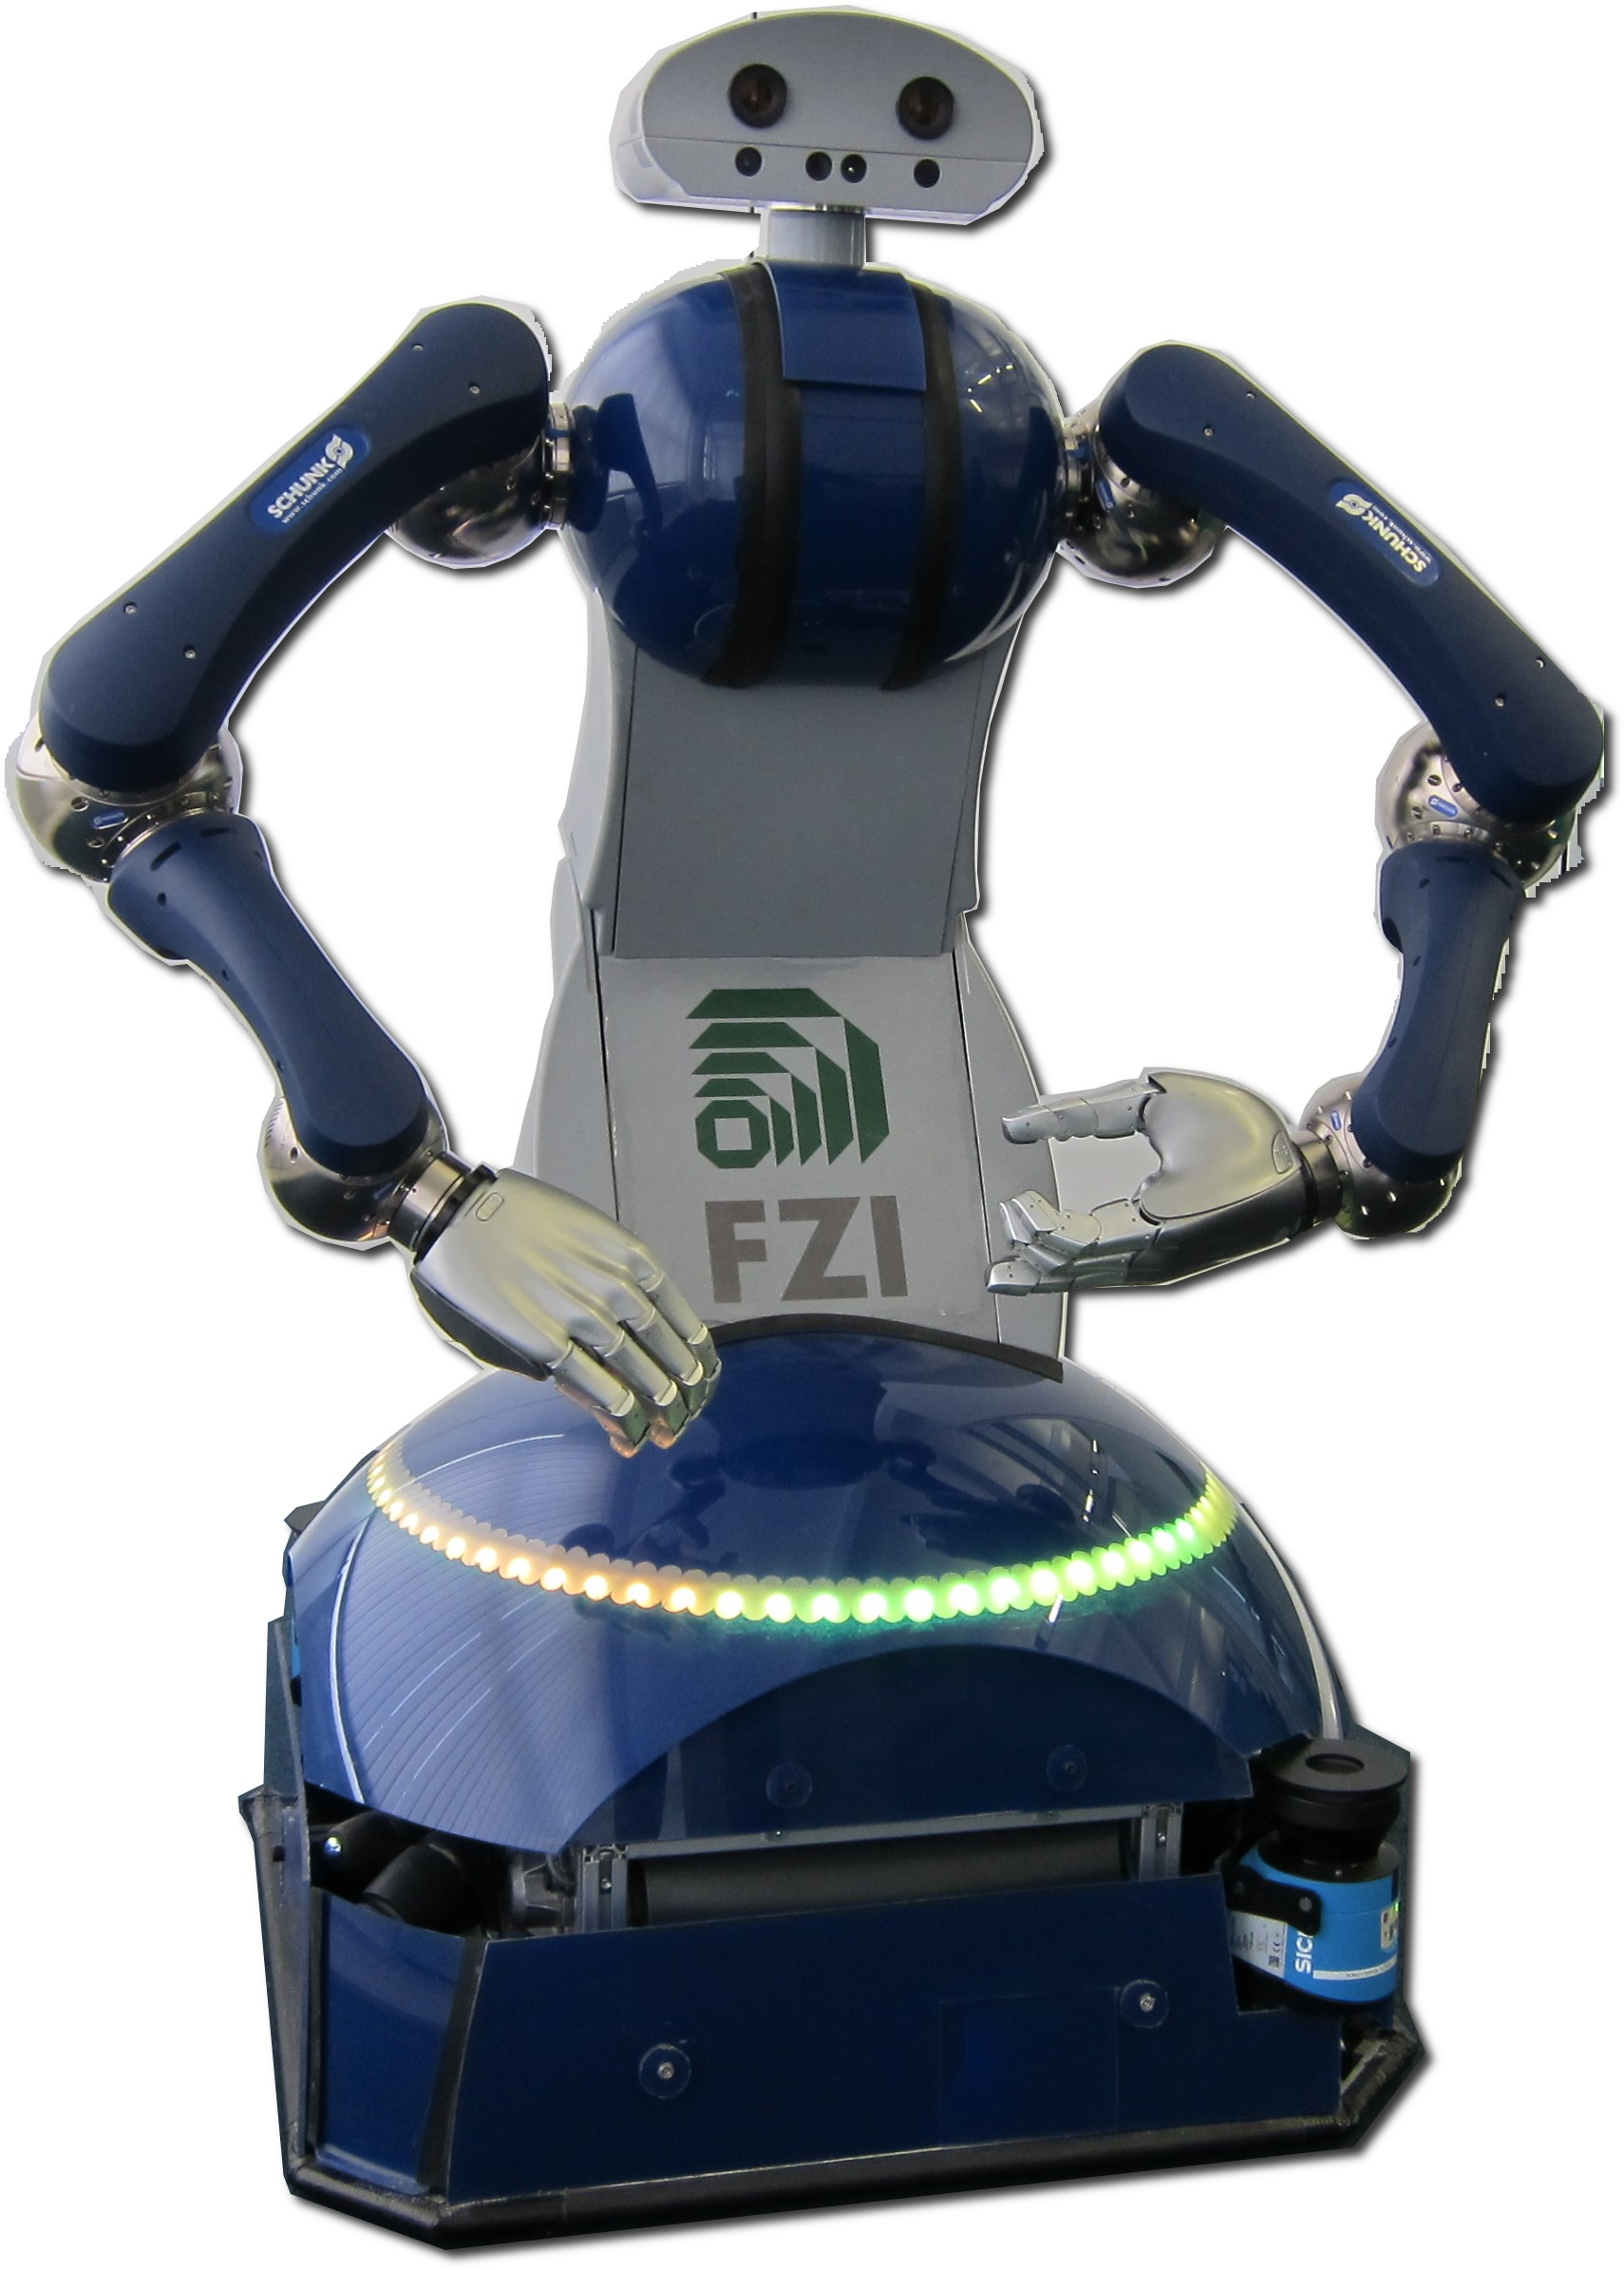
\includegraphics[width=0.5\textwidth]{graphics/hollie}
	\caption{\label{fig:hollie} Die mobile Roboterplattform \gls{hollie}}
\end{figure}



\section{Stand der Technik}
\label{stand_der_technik_sec}
\authorsection{\editorabel}

\subsection{Hardware}

\subsubsection{3D Kameras (am Beispiel Microsoft Kinect)}
Die Abbildung \ref{fig:Kinect} zeigt ein Bild der Kinect.
Sie ist mit laser-basiertem \gls{ir} Projektor und einem monochromen \gls{cmos} Sensor ausgestattet.
Der \gls{ir}-Projektor projiziert ein Muster auf die beobachtete Szenerie, während der  Sensor die Verformungen des Musters detektiert und gegen ein Vorgabemuster mittels Epipolargeometrie ein Tiefenbild errechnet.
Die Kinect ist darüber hinaus mit einem Neigemotor, einer Reihe von Mikrofonen und einer \gls{rgb}-Kamera ausgestattet.
Horizontal hat die Kamera einen Öffnungswinkel von $57\circ$ und vertikal $43\circ$.
Die Arbeitsentfernung der Kinect liegt zwischen 0.8 und 3.5 m.
Die Auflösung der Tiefenkamera beträgt 3mm in der X/Y Ebene und 10mm in Z-Richtung bei einem Abstand von 2 Metern.
Die Auflösung ist 640 x 480 Bildpunkte bei einer Bildfrequenz von 30 Hz.
Das Tiefenbild hat eine 11 bit Auflösung mit Werten zwischen 0 und 2047.

% Die Abbildung \ref{fig:Kinect} zeigt ein Bild der Kinect. Sie ist mit
%  laser-basiertem \gls{ir} Projektor und einem monochromen \gls{cmos} Sensor ausgestattet.
%  Der \gls{ir}-Projektor projiziert ein Muster auf die beobachtete Szenerie,
%  während der \gls{cmos} Sensor die Verformungen des Musters detektiert und gegen
%  ein Vorgabemuster mittels Epipolargeometrie ein Tiefenbild errechnet.
%  Die Kinect ist darüber hinaus mit einem Neigemotor, einer Reihe von Mikrofonen
%  und einer \gls{rgb}-Kamera ausgestattet. Horizontal hat die Kamera einen Öffnungswinkel
%  von $57^\circ$ und vertikal $43^\circ$. Die Arbeitsentfernung der Kinect liegt
%  zwischen $0,8$ und $3,5m$. Die Auflösung der Tiefenkamera beträgt $3mm$ in
%  der X/Y Ebene und $10mm$ in Z-Richtung bei einem Abstand von $2$ Metern. Die
%  Auflösung ist $640$ x $480$ Bildpunkte bei einer Bildfrequenz von $30Hz$. Das
%  Tiefenbild hat eine $11bit$ Auflösung mit Werten zwischen $0$ und $2047$.

\begin{figure}[h]
\center
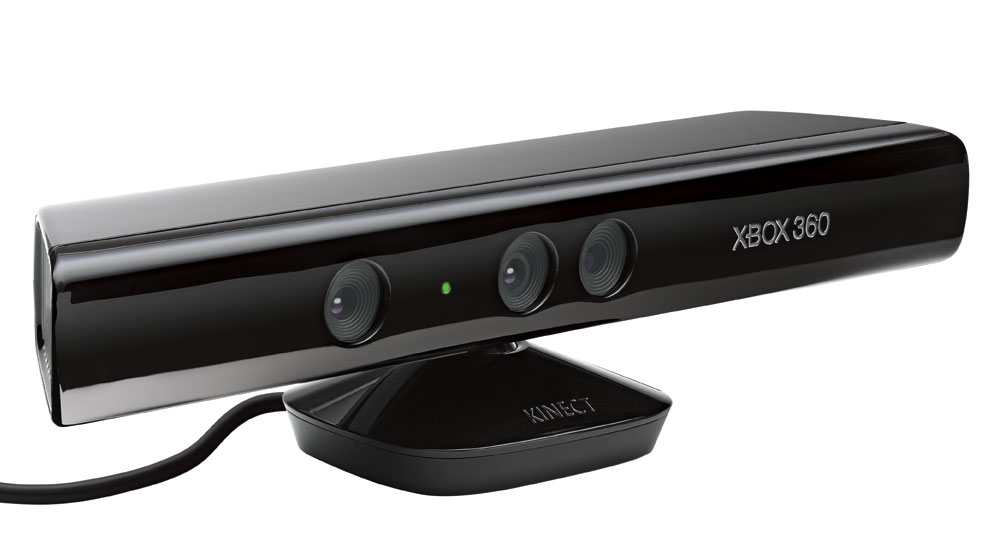
\includegraphics[scale=0.3]{graphics/Kinect.jpg}
\caption{\label{fig:Kinect} Kinect \cite{kinect_1}}
\end{figure}

Für die Kinect wurden in den letzten Jahren mehrere Entwicklerbibliotheken erstellt, die sich wachsender Beliebtheit erfreuen.
Es ist eine rasant wachsende Anzahl von Applikationen vorhanden, die 3D Kameras unterstützen.
Ursprünglich als Entertainmenthardware entwickelt, findet die Kinect vermehrt auch in der Forschung massiv Anwendung.
Ähnliche Spezifikationen haben auch die Wavi Xtion Kameras der Firma ASUS.



\subsubsection{Mobile Roboterplattformen}

Mobile Roboterplattformen werden in den meisten Fällen zu Forschungszwecken verwendet.
Wissenschaftler verschiedener Disziplinen wirken an Design und Programmierung mit.
Sie weisen teils stark unterschiedliche Konfigurationen auf.
Seit vielen Jahren wird jedoch intensiv an menschenähnliche Prototypen gearbeitet.
Nach der Konstruktion dienen solche Plattformen häufig dazu durch verschiedenste Programmierungen vorgegebene Aufgaben zu erfüllen.
Im Rahmen des Mobile Roboterpraktikums haben wir an der Plattform HoLLiE des FZI Karlsruhe gearbeitet.
Auch die Roboterplattform ARMAR wurde in Karlsruhe am KIT entwickelt.

Aufgrund der großen Popularität, technischen Ausgereiftheit und guten Dokumentation soll exemplarisch an dieser Stelle die Roboterplattform PR2 der Firma willow garage dargestellt werden, siehe Abbildung  \ref{fig:PR2Struktur}.

\begin{figure}[h]
\center
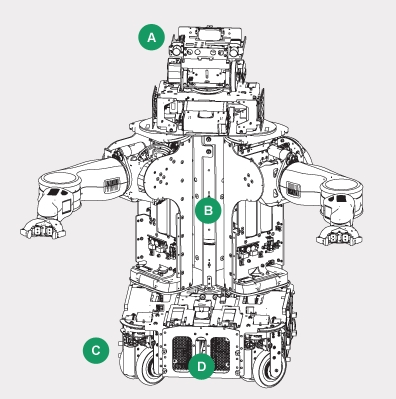
\includegraphics[scale=0.5]{graphics/PR2Struktur.jpg}
\caption{\label{fig:PR2Struktur} Struktur des PR2 \cite{kinect_5}}
\end{figure}

Der PR2 ist ein kommerziell erhältlicher, weit entwickelter humanoider Roboter, der den typischen Aufbau humanoider Roboterplattformen aufweist.
Er hat folgende, HoLLiE ähnlicher, technische Eigenschaften \cite{kinect_5}:

\begin{itemize}
  \item 2 Arme mit Greifern (Arm 4 \gls{dof}, Handgelenk 3 \gls{dof}, Greifer 1 \gls{dof})
  \item Kopf mir 2 \gls{dof}
  \item Omnidirektionale Basis (3 \gls{dof})
\end{itemize}

Außerdem ist der PR2 mit einer großen Anzahl an Sensoren ausgestattet und innerhalb gewisser Parameter modular konfigurierbar.
Der PR2 ist mit folgenden Sensoren ausgestattet bzw. ausstattbar:

\begin{itemize}
  \item Microsoft Kinect
  \item 5 MP Kamera
  \item Stereokamerasystem
  \item Kleinwinkelkamera
  \item \gls{led} Musterrojektor
  \item Laserscanner
  \item Mikrofonarray
  \item Beschleunigungssensorik in den Armen
  \item Kraftsensorik in den Greifern
  \item Kalibrierungs-\glspl{led}
\end{itemize}

Der PR2 wird mittlerweile an einigen namhaften Universitäten und Forschungsstätten eingesetzt (\ua TU München, Stanford University und \gls{mit}) und es existieren Arbeiten in verschiedensten Bereichen, wie zur Betreuung älterer und eingeschränkter Menschen, zum Verrichten von Hausarbeiten  und dem Einsatz in Dienstleistungsbetrieben.

Besonders an dem Roboter ist die gemeinsame mechatronische, aber besonders informationstechnische Plattform, die auf dem Betriebssystem \gls{ros} aufbaut und es Wissenschaftlern ermöglicht in einer gemeinsamen Umgebung zu arbeiten, Ergebnisse auszutauschen und auf neue Generationen zu übertragen.



\subsection{Software}

\subsubsection{OpenNI}

\gls{openni} dient zur Entwicklung von Applikationen der Mensch-Maschine-Interaktion.
Dazu stehen der \gls{api} viele Schnittstellen zur Verfügung.
Folgende Eigenschaften stellt die \gls{api} zur Verfügung \cite{kinect_6}:

\begin{itemize}
  \item Kommunikation mit Video- und Audiosensoren
  \item Middleware zur Video- und Audiodatenverarbeitung
\end{itemize}

Dem Entwickler stehen zur Entwicklung entsprechender Appliaktionen mit \gls{openni} eine Reihe von Werkzeugen zur Verfügung.Grundlegend ist dabei, dass ein gemeinsames Interface in Form von Middleware verwendet wird.
Dies ermöglicht die Entkopplung von Hardware- und Softwareherstellern, die nur die spezifizierten Datensignale liefern, bzw. darauf aufbauen müssen.
\gls{openni} steht zum kostenlosen Download zur Verfügung.
Die Struktur ist in unten stehender Abbildung dargestellt: 

\begin{description}
 \item[Oben:] Software-Applikationen die mit \gls{openni} kommunizieren
 \item[Mitte:] \gls{openni}, das Kommunikationsschnittstellen sowohl zu Hardware- als auch zu Softwarekomponenten zur Verfügung stellt
 \item[Unten:] Hardwarekomponenten, die Video- und Audiosignale aufnehmen
\end{description}

\begin{figure}[h]
	\center
	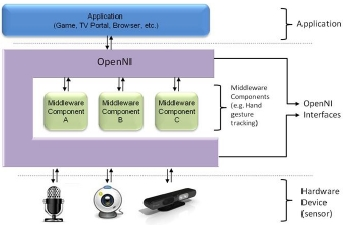
\includegraphics[width=0.7\textwidth]{graphics/openNI.jpg}
	\caption{\label{fig:openNI} \gls{openni} Architektur \cite{kinect_6}}
\end{figure}

\gls{openni} basiert auf drei Grundkonzepten:
\begin{itemize}
  \item Modularität
  \item Produktionsknoten
  \item Produktionsketten
\end{itemize}


\paragraph{Modularität}
Modularität bezieht sich in diesem Zusammenhang auf alle Aspekte OpenNIs.
Zum einen Hardware-Modularität;
Theoretisch werden alle Sensoren, die die spezifizierten Signale liefern unterstützt.
Auch die Software ist modular einsetzbar mit Komponenten zur Hand-, Körper-, Gesten- und Szenendetektion.
Mit den aufgezählten Modulen lassen sich relevante Informationen wie Gelenkposen, erkannte Gesten und die Segementierung der Szene gewinnen \cite{kinect_6}.

\paragraph{Produktionsknoten}
Produktionsknoten dienen in \gls{openni} zur Generierung von Daten.
Diese Daten stellen sie anderen Anwendungen zur Verfügung.
Da Prduktionsknoten in einer Hierarchie zu einander stehen können Produktionsknoten einer niedrigeren Hierarchieebene von solchen einer höheren Ebene genutzt werden wodurch.
Somit lassen sich von manchen Knoten low-level-Informationen wie Tiefenbilder, von anderen high-level-Informationen wie Gelenkposen generieren \cite{kinect_6}.

\paragraph{Produktionsketten}
Produktionskette ist der formalisierte Begriff für die Verarbeitungskaskade in einer Produktionsknotenhierarchie.
Höhere stehende Produktionsknoten fragen Informationen bei niedriger gestellten ab, die wieder niedriger gestellte abfragen usw.
Anwendern bleibt somit, mit der Verwendung der abstrakten Produktionsknoten hoher Hierarchieebenen die komplexe Verarbeitunsstruktur verborgen.
Diese Struktur ermöglicht Entwicklern außerdem eine größere Freiheit bei deren Gestaltung \cite{kinect_6}.

\paragraph{Microsoft SDK}
Auch der Hersteller der Kinect, Microsoft, bietet nun ein offizielles \gls{sdk}, das sich leicht in Visual Studio und Dot Net integrieren lässt.
Mit dem Kinect Sensor und Microsoft \gls{sdk} hat man Zugang zu Werkzeugen mit denen Menschen und Sprache erkannt werden.
Darüber hinaus existiert ein Entwicklerportal mit kostenlosen Tutorials und Beispielen.
Dort kann Microsoft \gls{sdk} auch kostenlos heruntergeladen werden \cite{kinect_4}.
Die Eigenschaften des Microsoft \gls{sdk} sind denen von \gls{openni} ähnlich, Microsoft \gls{sdk} bietet jedoch kein eigenes Gestenerkennungsmodul, wie es in \gls{openni} verfügbar ist.
In Vergleichstests von \gls{openni} und Microsoft \gls{sdk} schneidet \gls{openni} bisher besser ab, jedoch liefert Microsoft \gls{sdk} höhere Genauigkeit und Robustheit beim Skeletttracking.
Die Sprach- und Gestenerkennung findet nicht nur in Spielen sondern auch in der Bedienung des Computers Anwendung, wie zum Beispiel bei Microsofts Internetsuchmaschine bing.
Eine neu entwickelte Körperscan Software erlaubt es, Bilder aufzunehmen und diese als Animationen oder als Avatar in Spielen zu verwenden, siehe Abbildung \ref{fig:skelettracking} \cite{kinect_5}.

\begin{figure}[h]
	\center
	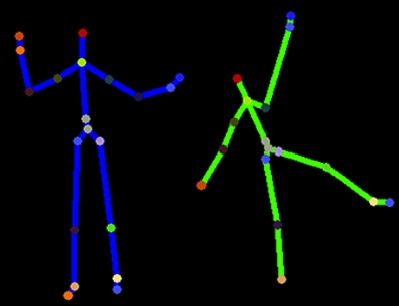
\includegraphics[scale=0.8]{graphics/skelettracking.jpg}
	\caption{\label{fig:skelettracking} Beispielhafte Anwendung von Skelettracking\cite{kinect_5}}
\end{figure}


%\gls{openni} ist ein plattformübergreifendes Framework zur Entwicklung von
%Applikationen, die auf natürlicher Mensch-Maschine-Interaktion aufbauen.
% Die \gls{openni}-\gls{api} stellt eine Vielzahl an Schnittstellen bereit, um
% entsprechende Applikationen zu programmieren. Der Hauptzweck von \gls{openni}
%  ist eine Standard-\gls{api} bereitzustellen, die folgende Eigenschaften vereint \citep{openNI2012}:
%
%\begin{itemize}
%  \item Kommunikation mit Video und Audiosensoren
%  \item Bereitstellung von Middleware zur Video- und Audiodatenverarbeitung,\\
%  wie die Unterstützung bei der Objektdetektion in Bildern
%\end{itemize}
%
%Dabei stellt \gls{openni} eine Reihe von \glspl{api} bereit, die sowohl von  (3D-Kamera-)
% Sensoren als auch Middleware Komponenten implementiert werden können.
% Durch das Entkoppeln von Sensor und Middleware können mit \gls{openni} angefertigte Softwareprodukte
% ohne zusätzliche Arbeit auf verschiedener Middleware aufbauen (\glqq write once, deploy everywhere\grqq).
% Middleware Entwickler können somit Algorithmen, die auf standardisierten (Bild-) Formaten aufbauen,
% unabhängig von der Sensorik-Hardware entwickeln. Hardware Hersteller müssen auf der anderen Seite
% Sensoren zur Verfügung stellen, die diese Bildformate generieren können. \gls{openni} steht kostenlos
% als open source Quelle zur Verfügung. In Abbildung \ref{fig:openNI} ist das
% Konzept von \gls{openni} in 3 Schichten dargestellt:
%
%\begin{description}
%  \item[Oben:] Software, die Natürliche Interaktion auf \gls{openni} aufbauend
%  verwendet
%  \item[Mitte:] \gls{openni}, das Kommunikationsschnittstellen sowohl zu
%  Hardware- als auch zu\\ Softwarekomponenten zur Verfügung stellt
%  \item[Unten:] Hardwarekomponenten, die Video- und Audiosignale aufnehmen
%\end{description}
%
%\begin{figure}[h]
%\center
%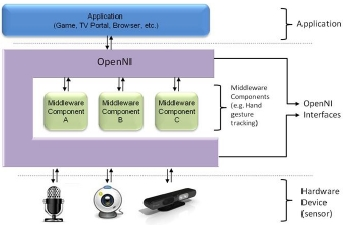
\includegraphics[scale=0.8]{graphics/openNI.jpg}
%\caption{\label{fig:openNI} \gls{openni} Architektur \citep{openNI2012}}
%\end{figure}
%
%OpenNI basiert auf einigen Grundkonzepten:
%
%\begin{itemize}
%  \item Modularität
%  \item Produktionsknoten
%  \item Produktionsketten
%\end{itemize}
%
%\newpage
%\todo[inline]{Ein wenig gepfuscht hier \ldots falls wer Lust hat kann er das
%ja ändern}
%\begin{description}
%\item[Modularität]
%\end{description}
%
%Unter Modularität ist in diesem Zusammenhang vor allem die Austauschbarkeit von Komponenten
% und die Architektur des Systems zu verstehen.
% Es werden folgende Module unterstützt:
%
%
%\begin{itemize}
%\item \textbf{Sensoren:}
%\begin{itemize}
%  \item 3D Sensoren
%  \item \gls{rgb} Kameras
%  \item Infrarot Kameras
%  \item Mikrofone / Mikrofonarrays
%\end{itemize}
%\item \textbf{Middleware Komponenten:}
%\begin{description}
%  \item[Ganzkörperanalyse Middleware:] Softwarekomponente, die Sensordaten
%  verarbeitet und daraus relevante Informationen wie Gelenkposen ableitet
%  \item[Handanalyse Middleware:] Software, die hilft Sensordaten zu verarbeiten,
%  um die Positionen von Händen zu ermitteln
%  \item[Gestendetektion:] Softwarekomponente, die Gesten erkennt und diese
%  Information an die Anwendungen weitergibt
%  \item[Szenenanalyse:] Software, die verschiedene Szenenrelevanten
%  Informationen ableitet, wie Hintergrundseparation, Erkennen der Bodenebene und Identifikation und Detektion von verschiedenen Personen
%\end{description}
%\end{itemize}
%
%
%\begin{description}
%\item[Produktionsknoten]
%\end{description}
%
%
%In \gls{openni} werden sogenannte Produktionsknoten definiert die die Aufgabe haben,
% für verschiedene Anwendungen die Daten zur Verfügung zu stellen.
% Produktionsknoten stehen dabei in einer Hierarchie zueinander.
% Sie können sowohl Produktionsknoten eines niedrigeren Levels verwenden als auch von Knoten höheren
% Levels verwendet werden. Konkret bietet \gls{openni} einen User Generator, der alle Daten einer getrackten Person
% liefern kann. Hierfür verwendet der User Generator einen Tiefenbildgenerator, aus dem er seine Informationen ableitet.
%
%\begin{description}
%\item[Produktionsketten]
%\end{description}
%
%Wie bereits dargestellt können mehrere Module gleichzeitig an der selben \gls{openni} Distribution angemeldet sein.
% Diese Topologie erlaubt Anwendungen flexibel auf Aufnahme- und Verarbeitungsmodule zuzugreifen.
% Als Produktionsketten werden die bereits angesprochenen hierarchischen Verarbeitungsketten der Produktionsknoten verstanden.
% Der erwähnte User Generator verwendet einen Tiefengenerator, der wiederum seine Daten von einem Tiefensensor bezieht.
% Diese Abhängigkeit bzw. sequenzielle Herunterbrechen der Aufgabe der Produktionsknoten wird als Produktionskette verstanden.
% Vorteilhaft ist an dieser Struktur, dass Anwendungen nur die oberste Schicht mit ihren Fähigkeiten nutzt.
% Die Konfiguration der darunter liegenden Schichten bleibt dabei verborgen und erlaubt Herstellern größere Freiheit
% in der Gestaltung der niedrigeren Hierarchieebenen \citep{openNI2012}.
%
%\subsubsection{Microsoft \glsentrytext{sdk}}
%
%Auch der Hersteller der Kinect, Microsoft, bietet nun ein offizielles \gls{sdk},
% das sich leicht in Visual Studio und Dot Net integrieren lässt. Mit dem Kinect Sensor und Microsoft \gls{sdk}
% hat man Zugang zu Werkzeugen, mit denen Menschen und Sprache erkannt werden.
% Darüber hinaus existiert ein Entwicklerportal mit kostenlosen Tutorials und Beispielen.
% Dort kann Microsoft \gls{sdk} auch kostenlos heruntergeladen werden \citep{kinectDevKfW2012}.
%
%Die Sprach- und Gestenerkennung findet nicht nur in Spielen sondern auch in der Bedienung des Computers Anwendung,
% wie zum Beispiel bei Microsofts Internetsuchmaschine bing\footnote{\url{www.bing.com/}}. Eine neu entwickelte Körperscan Software erlaubt es,
% Bilder aufzunehmen und diese als Animationen oder als Avatar in Spielen zu
% verwenden, siehe Abbildung \ref{fig:skelettracking} \citep{noGameKinect2012}.
%
%\begin{figure}[h]
%\center
%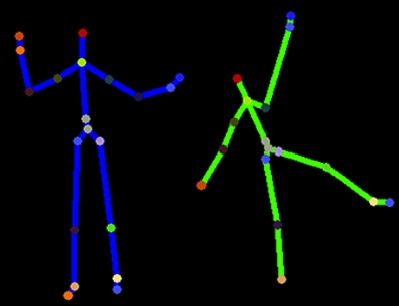
\includegraphics[scale=0.8]{graphics/skelettracking.jpg}
%\caption{\label{fig:skelettracking} Beispielhafte Anwendung von Skelettracking
%\citep{noGameKinect2012}}
%\end{figure}





\chapter{Grundlagen}
\label{grundlagen_cha}

Im folgenden Kapitel werden die Grundlagen beschrieben, die uns zur Verfügung standen, um die im ersten Kapitel näher beschriebene Zielsetzung zu erreichen. Dies betrifft zum einen die
Software-Grundlage MCA2, sowie die bereits vorhandene Roboterplattform Odete, die vor allem im Bereich Lokalisierung sehr stark adaptiert werden konnte.

\section{MCA2 - Modular Controller Architecture Version 2}
\authorsection{\editoranne}

Entwickelt, um die Bedürfnisse nach Wiederverwendbarkeit und Erweiterbarkeit eines Softwareprojekts zu unterstützen, ist MCA2 ein modulares Software-Rahmenwerk. Dieses unterstützt wiederverwendbare Komponenten mit standardisierten Komponenten, die leicht erweiterbar sind. Dadurch wird das Programmieren auf unterschiedlichen Roboter-Prototypen effektiver.

Erreicht wird dies, indem Teile des gesamten Kontrollsystems in kleinen standardisierte Modulen organisiert wird. Diese Module können dann im entsprechenden Kontext immer wieder verwendet werden, ohne erneut angepasst werden zu müssen. Das Rahmenwerk MCA2 sorgt für die Kommunikation und Synchronisation zwischen diesen Teilen.

\begin{figure}[h]
	\center
	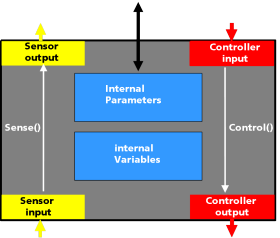
\includegraphics[scale=2.0]{graphics/mcamodule.png}
	\caption{\label{fig:MCA-Modul} Beispiel für ein MCA Modul}
\end{figure}

Jedes Modul ist dabei in gleicher Weise aufgebaut. Es besitzt 5 Schnittstellen, wovon vier zur Kommunikation mit anderen Modulen dienen, die fünfte wird genutzt um interne Parameter zu lesen und zu ändern. Die vier Kommunikationsschnittstellen ergeben sich jeweils aus der Kommunikation zu über- oder untergeordneten Modulen. In jede dieser beiden Richtung können Daten gesendet, bzw. empfangen werden. Man spricht in der einen Richtung von Sensor-, in der anderen Richtung von Kontroll-Daten. Diese Daten sind dabei realisiert durch einen Vektor fester Werte, die von einem Modul an ein Weiteres in derselben oder einer permutierten Reihenfolge weitergegeben werden. Mittels der fünften Schnittstelle werden diese Daten dann manipuliert. Dazu besitzt jedes Modul zwei Funktionen: Die Sense()- und die Control()-Funktion. Die Sense()-Funktion dient dazu, die Sensordaten von der Input- zur Output-Schnittstelle verändert oder unverändert weiter zu geben, die Control()-Funktion ist analog für die Kontrolldaten zuständig.

Das große Ziel von MCA2 war die Wiederverwendbarkeit von Modulen, dies wird um so effektiver, je einfacher die einzelnen Module gehalten sind. Um dennoch ein leistungsfähigeres Modul zu erhalten, das eine komplexere Funktionalität beinhaltet, werden Module in Gruppen zusammengestellt. 

\begin{figure}[h]
	\center
	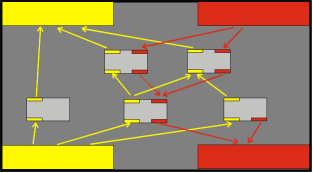
\includegraphics[scale=2.0]{graphics/mcagroup.png}
	\caption{\label{fig:MCA-Gruppe} Beispiel für eine MCA Gruppe}
\end{figure}


Eine Gruppe ist dabei wiederum aufgebaut wie ein Modul, besteht selbst jedoch aus vielen kleinen Modulen, um die komplexere Funktionalität zu erfüllen. Wird die Sense()- oder Control()-Funktion einer Gruppe aufgerufen, so löst das die Ausführung aller Sense()- und Control()-Funktionen innerhalb der Gruppe aus, beginnend bei der Eingangs-Schnittstelle, bis hin zur Ausgabe-Schnittstelle der Sensor-, bzw. Kontrolldaten.

Die Idee von Gruppen wird in MCA2 dann konsequent weiter gedacht und resultiert darin, dass Module und Gruppen wiederum hierarchisch zusammengesetzt werden, um noch komplexere Programme realisieren zu können. Eine ausführbare Datei, die aus Gruppen und Modulen zusammengesetzt ist, wird Part genannt. Der größte Unterschied zwischen einer Gruppe und einem Part besteht darin, dass die Sense()- und Control()-Funktionen einer Gruppe nur bei Aufruf, bei einem Part dagegen immer wiederholt entsprechend einer Art 'Takt' ausgeführt werden.

Für die die Arbeit im Rahmen des Projektpraktikums wurde noch zusätzlich ein Mechanismus benötigt, der einen geteilten Speicherbereich anbietet. Organisiert als einfacher Array von festen Werten bieten Blackboards diese Möglichkeit, um Daten für komplexere Datenstrukturen wie Bilder weiter zu leiten. Benötigt zum Beispiel für das Virtual Protective Field oder auch die Weitergabe von Daten der Laserscanner. \todo[inline]{Referenz zum VPF oder so was?}

Letztendlich bietet MCA noch Schnittstellen, die via Ethernet alle Sensordaten in Text oder Bild auf einer grafische Benutzeroberfläche bereitstellen. Diese mcagui kann auf jedem PC innerhalb des Netzwerkes ausgeführt werden, so dass die ausführende Computereinheit mit dem zusätzlichen Overhead nicht belastet wird. Mit Hilfe dieser grafischen Benutzeroberfläche wurde das Testen innerhalb einer Simulationsumgebung ausgeführt, aber auch erste Tests auf dem realen Roboter konnten mittels dieser Schnittstelle erleichtert werden.

\todo[inline]{Referenz zur benutzen GUI?}


\section{Odete}
\authorsection{\editordirk}
\todo[inline]{Dirk: Schreiben}


\section{SegwayOmni}
\authorsection{\editordirk}
\todo[inline]{Dirk: Schreiben}


% #############################################################################
%															Bahnplanung und Steuerung
% #############################################################################
\chapter{Bahnplanung und Steuerung}
\label{bahnplanung_steuerung_cha}

% ********************************************************************************
% 										Aufgabenstellung
% ********************************************************************************
\section{Aufgabenstellung}
\label{bahnplanung_aufgabenstellung_sec}
\authorsection{\editoroier}


Was die Aufgabestellung für die Bahnplanung und Steuerung betrifft, so kann man das in Abstraktionsschichten einteilen:
LowLevel-Ansteuerung, Inverse Kinematik, Bahnplanung und Kollisionsvermeidung.
Außerdem sollte man das alles auch simulieren können.

Für die LowLevel Ansteuerung ist die plattformspezifische Ansteuerung und Simulation notwendig. Außerdem sollte man auch die Pose aus Odometriedaten bestimmen können.

Die inverse Kinematik dient dazu, aus einer gegebenen Pose eine oder mehrere bis hin zu unendlich vielen Roboterkonfigurationen zu berechnen. Letzteres passiert, wenn es Raumpunkte gibt die zu Singularitäten führen. Das heißt, dass zum Beispiel bei einem 6-achsigen Roboter zwei Achsen kollinear werden. Im Falle einer mobilen Plattform würde man als inverse Kinematik die Berechnung einer Radstellung zu einer Pose (x, y, yaw) betrachten. Die Bestimmung der Geschwindigkeit wird danach durch inverse Odometrie gemacht. Zu lösende Aufgaben im Bereich der inversen Kinematik sind: die Umrechnung der Trajektorie in Geschwindigkeiten, die Limitierung der Beschleunigung des Roboters und das Limitieren der Geschwindigkeiten unter Beachtung des Protective Fields \ref{sec:vpf}.

Was die Bahnplanung betrifft, gibt es mehrere Aufgaben. Als erstes müssen die Menschendaten, sprich die Daten der Kinect-Kamera verarbeitet werden. Danach soll die Trajektorie, auf welcher der Roboter fahren soll, bestimmt werden, welches nebenbei kollisionsfrei sein sollte. Als letztes soll das Speichern der abgefahrenen Trajektorie und das Laden der abgefahrene Trajektorie implementiert werden.


%Als Ausgangssituation hatte man die Grundlagen der Odete für die LowLevel-Ansteurung und die inverse Kinematik. Sonst waren, Bahnplanung/Steuerung und Kollisionsvermeidung zunächst nicht vorhanden. Eine Simulationsumgebung war vorhanden, es fehlte aber noch die Programmierung der Gui .
%
%Nach dem Bottom-Up Prinzip hat man zunächst, die LowLevel-Ansteuerung von der Odete angepasst und mittels Simulation getestet.

%Das \textit{DriveAlongPath} Modul, welches sich mit der inverse Kinematik beschäftigt, dient um aus eine Trajektorie aus 3 Punkte die nötige Koordinaten für \textit{OmniDrive} zu berechnen.
%Falls es sich bspw. um ein Industrieroboter handeln würde, dann würde die inverse Kinematik die nötige Gelenkwinkeleinstellungen berechnen, um mit dem Greifer eine neue Position zu erreichen.
%Danach würde die inverse Dynamik die entsprechende Motor-Kräfte und Momente berechnen.
%
%Die Bahnplanung berechnet Trajektoriepunkte auf Basis der Mensch-Position und Geschwindigkeit, welche von der Kinect-Kamera geliefert werden.
%Außerdem werden hier diverse Transformationen von Welt zu Roboter bzw. Bild-Koordinaten und zurück gemacht.
%Nebenbei, wird der Pfad gespeichert damit der Roboter es später alleine abfahren kann.
%
%Zum Schluß wird eine ständige Überprüfung der geplante Trajektorie gemacht, um Kollisionen zu vermeiden.
%Um Hindernisse zu umfahren, werden der A*-Algorithmus und ein Potentialfeld eingesetzt.
%Letzteres wirkt, dass es \glqq teuer\grqq \space ist in der nähe von Hindernisse zu fahren.



% ********************************************************************************
% 										Grundlagen Bahnplanung
% ********************************************************************************
\section{Grundlagen der Bahnplanung und Steuerung}


\subsection{Steuerung}
\label{bahnplanung_steuerung_sec}

Weil die gefundene Trajektorie normalerweise nicht glatt ist, werden für die Steuerung unterschiedliche Interpolationsarten verwendet.
Die Bahnsteuerung kann im kartesischen Raum oder im Konfigurationsraum stattfinden.
Im kartesischen Raum ist es näher an der zu lösenden Aufgabe, man muss dann aber für jeden Punkt die inverse Kinematik berechnen.
Die Steuerung im Konfigurationsraum hingegen liegt näher an den Gelenken, dafür ist die Formulierung der Trajektorie umständlicher.
Vor und Nachteile beider Optionen kann man in der Tabelle \ref{fig:steurungProContra} sehen.


\begin{table}[h]
		\centering
		\begin{tabular}{| p{7cm} | p{7cm}|}
\hline
\textbf{Kartesischer Raum} & \textbf{Konfigurationsraum}\\
\hline
+ Bahn einfacher zu formulieren & + Ansteuerung der Gelenke ist
einfacher\\
+ Interpolation ist einfacher & + Trajektorie ist eindeutig und
berücksichtigt Grenzen\\

- Inverse Kinematik ist für jeden Trajektorienpunkt zu lösen & - Interpolation für mehrere
Gelenke\\
- Geplante Trajektorie nicht immer ausführbar & - Formulierung der Trajektorie umständlicher\\
\hline
		\end{tabular}
		\caption{\label{fig:steurungProContra} Vor und Nachteile der Steuerung im Kartesischen und Konfigurationsraum Quelle: \citep{rob1}}
		\end{table}	
Es gibt unterschiedliche Interpolationsarten:
Zirkular, Linear und Spline-Bahn oder auch approximative Bahnsteuerung.
Bei der Linearinterpolation wird einfach zwischen zwei Teiltrajektorien interpoliert, wie man auf der Abbildung \ref{fig:linearinterpolation} sehen kann.
\begin{figure}[h]
	\center
	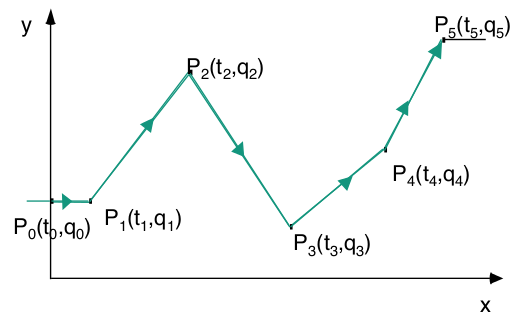
\includegraphics[scale=0.35]{graphics/linearinterpolation.png}
	\caption{\label{fig:linearinterpolation} Beispiel der Linearinterpolation Quelle: \citep{rob1}}
\end{figure}
Die Zirkularinterpolation schafft hingegen kreisförmige Verfahrwege zwischen zwei Punkten.
Wenn man allerdings segmentweise interpoliert, werden die Endbedingungen der Teiltrajektorie $i-1$ und die Anfangsbedingungen der Teiltrajektorie $i$ aneinander angepasst, so dass die Teiltrajektorien durch Splines beschrieben werden, wie man auf der Abbildung \ref{fig:segmentinterpolation} sehen kann.
\begin{figure}[h]
	\center
	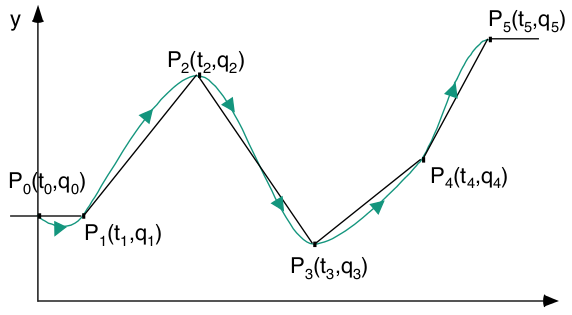
\includegraphics[scale=0.35]{graphics/segmentinterpolation.png}
	\caption{\label{fig:segmentinterpolation} Beispiel der segmentweisen Bahninterpolation \citep{rob1}}
\end{figure}
 
Bei der approximativen Bahnsteuerung werden anders als bei der Bahninterpolation nicht alle Kontrollpunkte der Trajektorie befahren, sondern die Kontrollpunkte beeinflussen den Bahnverlauf und werden approximiert.
Neben Bernsteinpolynomen wird hier besonders Überschleifen benutzt, um sanft Kurven zu fahren wie man auf der Abbildung \ref{fig:ueberschleifeninterpolation} sieht.
Letzteres wurde auch im Praktikum eingesetzt.
\begin{figure}[h]
	\center
	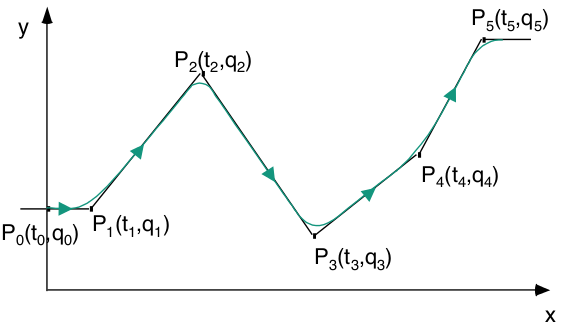
\includegraphics[scale=0.35]{graphics/ueberschleifeninterpolation.png}
	\caption{\label{fig:ueberschleifeninterpolation} Beispiel der approximierten Bahnsteuerung mit Überschleifen \citep{rob1}}
\end{figure}

\subsection{Bahnplanung}
\label{bahnplanung_grundlagen_sec}
\authorsection{\editoroier}

Bahnplanung befasst sich mit dem Problem, eine kollisionsfreie Bahn zu finden, die ein Robotersystem von der aktuellen Position in die Zielposition überführt.
Damit gehört es zu einer der Basisprobleme der Robotik.
Die Verfahren kann man nach unterschiedlichen Gesichtspunkten klassifizieren \cite{rob1}.

Nach Robotertyp:
\begin{itemize}
\item Bahnplanung für Manipulatoren (\zB Schweißen bei Industrierobotern)
\item Bahnplanung für mobile Roboter
\item Bahnplanung für Laufmaschinen und anthropomorphe Systeme
\item Greif- und Montageplanung
\end{itemize}

Nach dem Zustandsraum wo die Planung stattfindet:
\begin{itemize}
\item Gelenkwinkelzustandsraum (Konfigurationsraum, der alle möglichen Gelenkwinkelkonfigurationen des Roboters beinhaltet)
\item Euklidischer Raum (Arbeitsraum, 3D / 6D)
\item Sensorzustandsraum
\item Objektzustandsraum
\end{itemize}

Nach Vollständigkeit:
\begin{itemize}
\item Vollständige Verfahren (liefern immer eine korrekte Lösung und können ermitteln, ob keine Lösung existiert)
\item Probabilistisch vollständige Verfahren (Falls eine Lösung existiert konvergiert die Wahrscheinlichkeit, dass eine Lösung gefunden wird, bei fortschreitender Zeit gegen 1. Existiert keine Lösung, kann dies nicht ermittelt werden)
\end{itemize}

Nach Navigationsart:
\begin{itemize}
\item Globale Pfadplanung bedeutet, eine Trajektorie zum Ziel zu planen, wenn dem Roboter eine Karte der Umgebung vorliegt und er sich dort lokalisieren kann.
\item Lokale Pfadplanung wird eingesetzt um Hindernisse zu umfahren und wird bei mobilen Robotern meist in Kombination mit einem globalen Planer benutzt. 
\end{itemize}

Weil die explizite Berechnung des kollisionsfreien Konfigurationsraums bei Robotern mit mehr als drei Freiheitsgraden sehr teuer ist, benutzt man oft den impliziten Konfigurationsraum.
\Dh, dass die Bahnplanung im Konfigurationsraum stattfindet, aber die Kollisionen und Abstände im Arbeitsraum berechnet und in den diskretisierten Konfigurationsraum transformiert werden \citep{innoKonz}.
So wird der Konfigurationsraum während der Suche exploriert.

Der Ablauf eines Planungsverfahren ist normalerweise zweigeteilt\cite{Russell2003}.
\begin{enumerate}
\item Eine Roadmap oder einen Graph aufbauen mittels \gls{Voronoi}, \gls{Sichtgraphen}, \gls{Zellenzerlegung} oder zufällige Knoten je nach Sampling-Strategie (\zB für \gls{PRM} Verfahren\cite{Thrun2005}).
\item Im Graph einen Weg vom Startknoten zum Zielknoten finden mittels A*-Algorithmus oder anderer Suchalgorithmen.
\end{enumerate}

\subsubsection{Lokale Planer}
\label{bahnplanung_lokale_planer_sec}

In diesem Abschnitt werden einige gängige lokale Planer vorgestellt.

\paragraph{A*-Algorithmus} 

Der \textit{A*-Algorithmus}\citep{Russell2003} ist eine Erweiterung des \textit{Dijkstra Algorithmus} und gehört zu der Klasse der informierten Graphensuchalgorithmen.
Dies heißt, dass eine Schätzungsfunktion benutzt wird, um die Suche zu lenken.
Die Grundidee ist, immer den Knoten zu untersuchen, der wahrscheinlich am schnellsten ins Ziel führt.
Um den vielversprechendsten Knoten zu ermitteln, werden alle bekannten Knoten mit einer $f(x)$ Funktion bewertet und vom kleinsten $f$-Wert zum größten sortiert.
Der Knoten mit dem kleinsten $f$-Wert wird als nächstes untersucht. 

Um den vielversprechendsten Knoten zu ermitteln, wird die Formel
\begin{equation}
 f(x) = g(x) + h(x)
\end{equation}
benutzt.
Dabei sind $g(x)$ die Pfadkosten, um $x$ vom Startknoten zu erreichen.
$h(x)$ ist die Heuristik, sprich die Schätzung der Pfadkosten, das Ziel von $x$ aus zu erreichen.
Wichtig dabei ist, dass die Heuristik immer optimistisch sein muss, das heißt, dass die Schätzung kleiner oder gleich sein muss als die wirklichen Pfadkosten, weil sonst der Algorithmus nicht mehr optimal ist.
Als Heuristik wird oft der Euklidische Abstand oder die Manhattan Distanz benutzt.
In Abbildung \ref{fig:a*} ist eine erfolgreich beendete \textit{A*}-Suche mit Angaben zum Ablauf dargestellt.

\begin{figure}[h]
\center
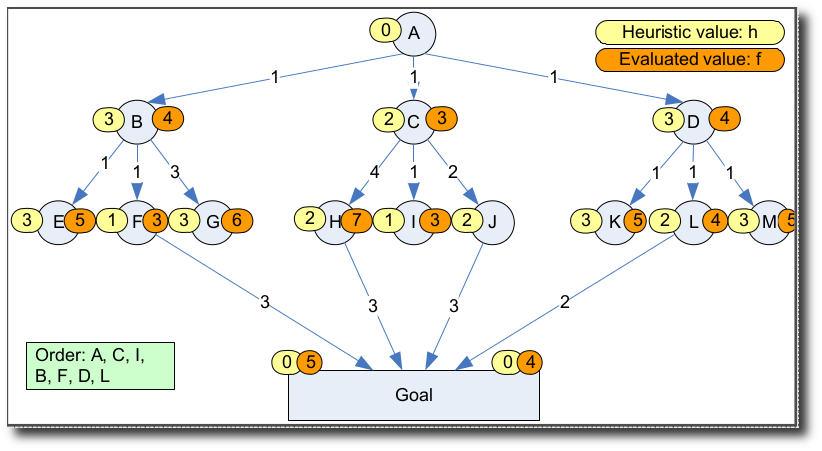
\includegraphics[scale=0.3]{graphics/AStar.png}
\caption{\label{fig:a*} Erfolgreich beendeter Ablauf eines \textit{A*}  \citep{innoKonz}}
\end{figure}

Der \textit{A*-Algorithmus}, obwohl er nicht mehr als state-of-the-art gilt\citep{innoKonz}, ist als lokaler Planer, vor allem in 2D, sehr gut.
Mit mehr Dimensionen oder Freiheitsgraden arbeitet er viel schlechter.
Außerdem kann man den Grundalgorithmus noch weiter optimieren.
Zum Beispiel mit dem Hierarchischen \textit{A*}, damit er, wenn keine Hindernisse in der Nähe liegen, größere Schritte und sonst kleinere Schritte macht.
Es gibt zusätzliche Erweiterungen für die bidirektionale Suche, die parallele \textit{A*}-Suche und dynamische Auswahl von Start und Zielknoten.
Man könnte auch den Algorithmus stoppen, sobald man einen Weg gefunden hat, dann ist der Algorithmus natürlich nicht mehr optimal.
Diese Erweiterungen sind von der zu lösenden Aufgabe abhängig, mehrere Start und Zielknoten machen zum Beispiel bei mobilen Robotern nicht viel Sinn, dafür könnte es beim Schweißen nützlich sein.

\paragraph{Potentialfelder}

Bei diesen Verfahren bewegt sich der Roboter unter dem Einfluss von Kräften, die ein Potentialfeld auf ihn ausübt.
Die Grundidee ist, dass Hindernisse ein Abstoßungspotential auf den Roboter ausüben und das Ziel hingegen ein Anziehungspotential.
Der negative Gradient der resultierenden Potentialkraft bestimmt die künstliche Kraft, die auf den Roboter ausgeübt wird.

\begin{equation}
F(q) = - \nabla U(q)
\end{equation}
wobei $U(q)$ die Summe der Abstoßungs- und Anziehungspotentiale ist.
Diese Summe ist in Abbildung \ref{fig:potentialfeld} dargestellt.

\begin{figure}[h]
\center
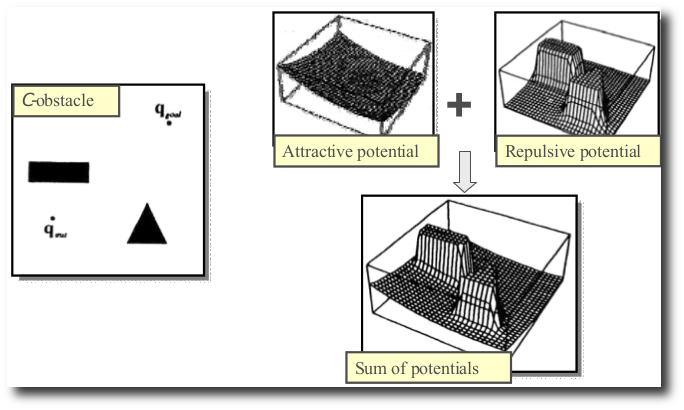
\includegraphics[scale=0.4]{graphics/potentialfeld.png}
\caption{\label{fig:potentialfeld} Summe der Abstoßungs- und Anziehungskräften \citep{innoKonz}}
\end{figure}

Die Vorteile des Verfahrens wären zum Beispiel der geringe Rechenaufwand für die Pfadplanung, dass die Bahnplanung und Steuerung in einer Funktion verbunden werden\citep{mobileRobotics}, was die allgemeine Steuerungsstruktur vereinfacht.
Noch ein Vorteil ist, dass die Pfade schon glatt sind, sprich man muss sie nicht mehr glätten.
Ein Nachteil hingegen ist, dass es im lokalen Minimum stecken bleiben kann.
Dies ist einer der Gründe, warum es als lokaler Planer benutzt wird.
Um dieses Problem zu beheben muss man Erweiterungen wie  \textit{random walk} oder \textit{backtracking} benutzen.
Eine andere Möglichkeit zur Flucht, die von Rimon und Koditschek vorgestellt wurde, ist es, den Zielpunkt als einziges lokales Minimum im Potentialfeld zu definieren.




% ********************************************************************************
% 										Umsetzung
% ********************************************************************************
\section{Umsetzung}
\label{bahnplanung_umsetzung_sec}


% -----------------------------------------------------------------------------
%													Motoransteuerung
\subsection{Motoransteuerung}
\label{bahnplanung_motoansteuerung_subsec}
\authorsection{\editoroier}



Was die Motoransteuerung angeht, so gab es schon das plattformunabhängige Modul \lstinline{SegwayOmniHal} von der Odete.
Unsere Aufgabe bestand darin, dieses Modul um die plattformspezifische Simulation \lstinline{Segway500RMPSimulation} zu ergänzen.
Als Eingaben erhält es Geschwindigkeiten, und Ausgaben sind die plattformspezifischen Geschwindigkeiten.
Auf der Abbildung \ref{fig:mca2architecture} sieht man die gesamte Struktur der Software und auf \ref{fig:segwayHal} ist das Modul \lstinline{SegwayOmniHal} abgebildet.

\begin{figure}[h]
	\center
	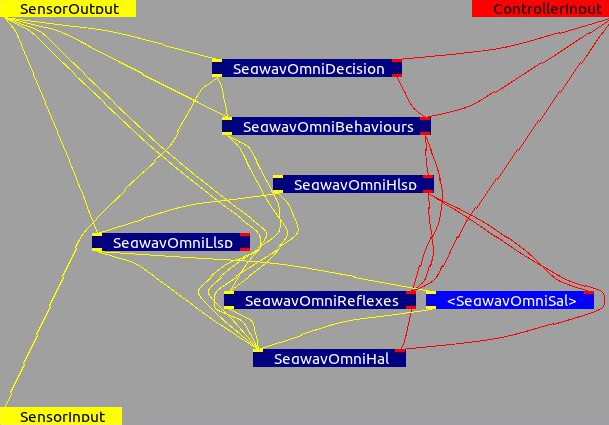
\includegraphics[scale=0.5]{graphics/mca2architecture.png}
	\caption{\label{fig:mca2architecture} Architektur der Software wo man die Vernetzung der einzelnen Module sehen kann}
\end{figure}

\begin{figure}[h]
	\center
	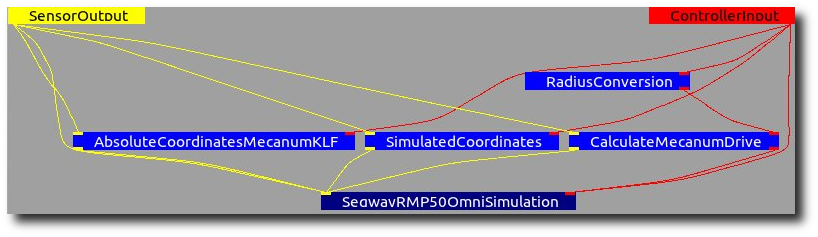
\includegraphics[scale=0.5]{graphics/segwayHal.png}
	\caption{\label{fig:segwayHal} Das Modul \lstinline{SegwayOmniHal}, welches für die Motoransteuerung zuständig ist}
\end{figure}
% evtl. auch so ein Diagramm wie Abb. 4.4 von WS10/11?
%		bzw. Abb. 2.3 von WS09/10


% -----------------------------------------------------------------------------
%													Inverse Kinematik
\subsection{Inverse Kinematik und manuelle Steuerung}
\label{inverse_kinematik_subsec}
\authorsection{\editorjulian}

\todo[inline]{Julian: Schreiben}
In der Gruppe \lstinline{SegwayOmniReflexes} befinden sich die Gruppen für die inverse Kinematik und die manuelle Steuerung des Roboters. Die Ausgaben der beiden Gruppen sind durch einen Multiplexer verbunden, die Selektion erfolgt durch die Berücksichtigung des Status der manuellen Steuerung. Ist diese aktiviert erfolgt unabhängig vom Zustand des Roboters das unmittelbare umschalten auf die manuelle Steuerung und die Ausgabe der Gruppe \lstinline{SegwayOmniManualReflexes} wird verwendet. Ist der manuelle Betrieb nicht aktiv kommt die Ausgabe der Gruppe \lstinline{SegwayOmniAutoReflexes} zur Verwendung. So ist es möglich zu jedem Zeitpunkt den Roboter zu stoppen und ihn manuell zu steuern.

\begin{figure}[h]
	\label{fig:bahnplanung_reflexes_gruppe}
	\center
	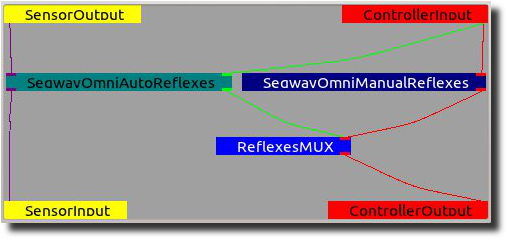
\includegraphics[scale=0.7]{graphics/BILD-SegwayOmniReflexes.png}
	\caption{Die Gruppe \lstinline{SegwayOmniReflexes}, zu sehen sind die Gruppen für den manuellen bzw. automatischen Betrieb, \lstinline{SegwayOmniManualReflexes} und \lstinline{SegwayOmniAutoReflexes}.}
\end{figure}

Die manuelle Steuerung ist mittels der zur Simulation erstellten \lstinline{MCAGUI} Oberfläche oder - beim Test am realen Roboter - mit einem Gamepad möglich.

Die inverse Kinematik bezieht sich auf die \lstinline{MCA2}-Gruppe \lstinline{SegwayOmniAutoReflexes} in der die Umrechnung von einer Trajektorie, bestehend aus drei Koordinaten, in Geschwindigkeiten stattfindet. Die in dieser Gruppe berechneten Geschwindigkeiten sind plattformübergreifend; gehören allerdings einer bestimmten Bewegungsart an. Folgende Bewegungsarten sind bereitgestellt:

\begin{description}
	\item[Differentiell] Die Steuerung des Roboters erfolgt indem Antriebsräder auf beiden Seiten des Roboters mit unterschiedlichen Geschwindigkeiten betrieben werden\footnote{\url{http://en.wikipedia.org/wiki/Differential_wheeled_robot}}.
	\item[Omnidirektional] Durch den Einsatz von Mecanum-Rädern\footnote{\url{http://de.wikipedia.org/wiki/Mecanum-Rad}} kann sich der Roboter holonom\footnote{Anzahl der Bewegungsfreiheitsgrade $\geq$ Anzahl Freiheitsgrade, hier: Bewegungsfreiheitsgrade $= 3$, Freiheitsgrade $= 3$.} bewegen.
\end{description}

\begin{figure}[h]
\label{fig:bahnpl_umsetz_schema_inv_kinem}
\centering
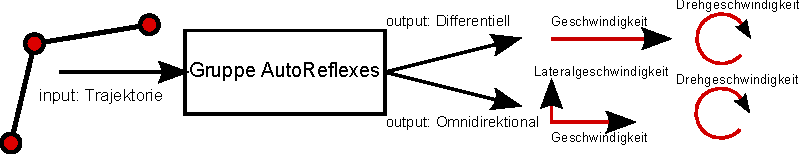
\includegraphics[scale=0.9]{graphics/SCHEMA-invKinem.pdf}
\caption{Schematische Darstellung des in-und Outputs der \lstinline{SegwayOmniAutoReflexes}-Gruppe.}
\end{figure}

Zusätzlich zur Berechnung der Geschwindigkeiten erfolgt in dieser Gruppe die Begrenzung der tatsächlichen Geschwindigkeit bezüglich einer vorgegebenen maximal Geschwindigkeit sowie der auftretenden Beschleunigungen durch Änderungen der Geschwindigkeit oder Bewegungsrichtung.

Zuletzt findet mit Hilfe des Virtual Protective Field (siehe \ref{lokalisierung_umsetzung_sec}) eine Kollisionsvermeidung statt.

\begin{figure}[h]
	\label{fig:bahnplanung_umsetzung_auto_refl}
	\center
	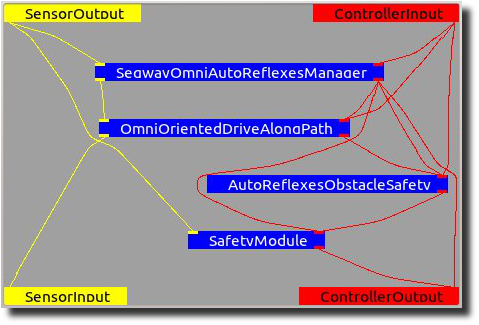
\includegraphics[scale=0.7]{graphics/BILD-SegwayOmniAutoReflexes.png}
	\caption{Die Gruppe \lstinline{SegwayOmniAutoReflexes} im Detail. Auf oberster Ebene befindet sich das Manager-Modul, welches die einzelnen Module kontrolliert.}
\end{figure}

Die Ausgabe von dieser Gruppe, also die bewegungsartspezifischen Geschwindigkeiten, werden an die Gruppe für die Motoransteuerung (siehe \ref{bahnplanung_motoansteuerung_subsec}) weitergereicht, um plattformspezifische Geschwindigkeiten zu berechnen.

\subsubsection{Vorhandene Software}
\label{bahnplanung_inv_kinem_vorhandene_software_sec}

Im Projekt \lstinline{SegwayOmni} bzw. \lstinline{Odete} gab es bereits eine \lstinline{Reflexes}-Gruppe in der ein Großteil der nötigen Funktionalität implementiert war. Insbesondere der zentrale Teil, die Module \lstinline{DriveAlongPath} bzw. \lstinline{OmniOrientedDriveAlongPath} welche für die inverse Kinematik zuständig sind, wurden zur Verfügung gestellt. Auch die Module zur Begrenzung der Beschleunigung waren vorhanden verursachten im laufenden Betrieb allerdings Probleme.

\subsubsection{Erweiterungen}
\label{bahnplanung_inv_kinem_erweiterung_sec}

Um eine einfache Steuerung der Gruppe zu gewährleisten steht an oberster Stelle das Modul \lstinline{AutoReflexesManager}. Dieses Modul vereinfacht und automatisiert verschiedene Funktionen der Module \lstinline{DriveAlongPath}, \lstinline{OmniOrientedDriveAlongPath}, \lstinline{SafetyModule} und \lstinline{ObstacleSafety}:
\begin{description}
	\item[DriveAlongPath]
	\begin{itemize}
		\item Setzen der maximal Geschwindigkeit
		\item Aktualisieren des Zählers zum Signalisieren das eine neue Trajektorie anliegt
		\item Aktivieren/Deaktivieren des Moduls
	\end{itemize}
	\item[SafetyModule] 
	\begin{itemize}
		\item Aktivieren/Deaktivieren des Moduls
	\end{itemize}
	\item[ObstacleSafety] 
	\begin{itemize}
	\item Aktivieren/Deaktivieren des Moduls	
	\end{itemize}
\end{description}
Weiterhin fließt in der \lstinline{AutoReflexes}-Gruppe die Information aus dem Virtual Protective Field mit ein, um kollisionsfreies Fahren zu ermöglichen.

\subsubsection{Virtual Protective Field}
\label{bahnplanung_virtual_protective_field_sec}

Das Modul \lstinline{ObstacleSafety} ist speziell für den Einsatz beim omnidirektionalen Fahren gedacht. In diesem Fahrmodus berechnet sich der tatsächliche Geschwindigkeitsvektor aus zwei orthogonalen Geschwindigkeitsvektoren, die jeweils die Vorwärtsgeschwindigkeit und die Lateralgeschwindigkeit beschreiben. Das Virtual Protective Field bietet gleichermaßen zu jeder Geschwindigkeitskomponente sowie zur resultierenden Geschwindigkeit die Information ob eine Kollision bevorsteht. Dadurch kann für jede Geschwindigkeitskomponente individuell entschieden werden, ob es nötig ist diese auf null zu setzen, also mit maximaler Bremsbeschleunigung zu bremsen, oder nicht. Durch dieses Vorgehen kann sich der Roboter an Ecken, die durch ungenaue Bahnplanung zu einer Kollision führen würden, vorbei schieben. Zugleich ist es die letzte softwareseitige Barriere, um eine Kollision zu vermeiden. Dies tritt dann ein, wenn für jede Geschwindigkeitskomponente, sowie für den resultierenden Geschwindigkeitsvektor ein Hindernis gemeldet wird.

\todo[inline]{Bild zur Verwendung des Virtual Protective Field}


%\begin{itemize}
%	\item Was konkret passiert -> Umwandlung der Trajektorie in (Plattformunabhängige) Geschwindigkeiten.
%	\item Limitierung der Beschleunigung
%	\item Was geht rein, was kommt raus
%	\item Virtual Protective Field verwenden um kollisionsfrei zu fahren.
%	\item was gab es schon
%	\begin{itemize}
%		\item Modul Reflexes von Odete Projekt
%		\item Bewegungsart abhängige Konvertierung einer Trajektorie
%		\item Differential Drive, Omni Drive
%		\item Safety Modul für Beschleunigung
%	\end{itemize}
%	\item Erweitert um Sicherheitsmodul welches das Virtual Protective Field berücksichtigt
%\end{itemize}


% -----------------------------------------------------------------------------
%													Bahnplanung
\subsection{Bahnplanung}
\label{bahnplanung_subsec}
\authorsection{\editortobias}


% \begin{itemize}
% 	\item Kurzer Grobüberblick über die Behaviours-Gruppe, hier werden Bahnplanungs-Aufgaben bearbeitet\todoprivate{ref zu behaviours-Bild}
% 	\begin{itemize}
% 		\item Berechnung von Trajektorien-Punkten auf Basis der Mensch-Position und Geschwindigkeit (Kinect)
% 		\item Schätzung der zukünftigen Position des Menschen
% 		\item Transformation von Welt- in Roboter- bzw. Bildkoordinaten und zurück\todoprivate{evtl. auch weg lassen}
% 		\item Abspeichern von Pfaden
% 		\item Abfahren von Pfaden
% 	\end{itemize}
% 	\item Module werden im Folgenden kurz beschrieben
% 	\item Kollisionsvermeidung als eigener Abschnitt
% \end{itemize}

Die Aufgaben der Bahnplanung werden in der \lstinline{MCA2}-Gruppe \lstinline{SegwayOmniBehaviours} bearbeitet (s. Abb. \ref{fig:behaviours}).
Im Einzelnen sind dies:
\begin{itemize}
	\item Berechnung von Trajektorien-Punkten auf Basis der Mensch-Position und Geschwindigkeit: \lstinline{GenerateTrajectory}
	\item Schätzung der zukünftigen Position des Menschen: \lstinline{HumanPosition}
	\item Abspeichern von Pfaden: \lstinline{StoreRoboterPositionsToFile}
	\item Abfahren von Pfaden: \lstinline{LoadRoboterPositionsFromFile}
	\item Kollisionsvermeidung: \lstinline{ObstacleAvoidance}
\end{itemize}

\begin{figure}[h]
	\center
	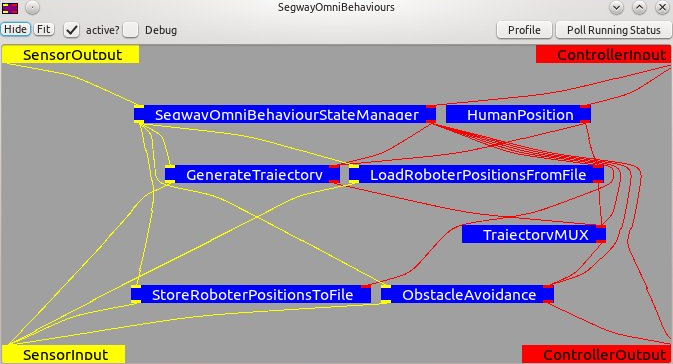
\includegraphics[width=0.8\textwidth]{graphics/behaviours}
	\caption{Die \lstinline{MCA2}-Gruppe \lstinline{SegwayOmniBehaviours}}
	\label{fig:behaviours}
\end{figure}

Die Module innerhalb der Gruppe werden im Folgenden beschrieben.
Die Kollisionsvermeidung wird in einem gesonderten Abschnitt (s. Abs. \ref{kollisionsvermeidung_subsec}) behandelt.


\subsubsection{Position des Menschen}
\label{bahnplanung_humanPosition_subsubsec}

% \begin{itemize}
%     \item bekommt aktuelle Position und Geschwindigkeit des Menschen von Kinect
%     \item schätzt die zukünftige Position des Menschen anhand dieser Daten
%     \item gibt aktuelle und geschätzte Position des Menschen aus
%     \item Zeit-Parameter für die Schätzung: $t_{est}$
%     \item Berechnung nach der Formel: $s_{est} = s_{act} + v \cdot t_{est}$
% \end{itemize}

Das Modul \lstinline{HumanPosition} bekommt als Parameter die aktuelle Position sowie die aktuelle Geschwindigkeit der vom Roboter verfolgten Person übergeben.
Anhand dieser Daten wird die zukünftige Position des Menschen geschätzt.
Als Resultat gibt das Modul die geschätzte zukünftige Position des Menschen aus.
Die aktuelle Position wird ebenfalls mit ausgegeben.

Für die Berechnung der zukünftigen Position des Menschen wird die Formel
\begin{equation}
	s_{est} = s_{act} + v \cdot t_{est}
\end{equation}
angewendet.
$s_{est}$ ist dabei die geschätzte zukünftige Position, $s_{act}$ beschreibt die aktuelle Position und $v$ die Bewegungsgeschwindigkeit des Menschen.
$t_{est}$ ist ein Parameter für die Zeitspanne, die in die Zukunft prädiziert werden soll.
Dieser Parameter wird aus einer externen Konfigurationsdatei geladen.


\subsubsection{Berechnung der Trajektorie}
\label{bahnplanung_trajektorie_subsubsec}

Die Berechnung der Trajektorie erfolgt im Modul \lstinline{GenerateTrajectory}.
Die aktuelle und geschätzte Position des Menschen, sowie die aktuelle Position des Menschen werden als Parameter übergeben, und dienen als Grundlage für die Berechnung der Trajektorie.
Die Struktur der zu berechnenden Trajektorie $s$ ist durch das Modul \lstinline{OmniDriveAlongPath} (s. Abs. \ref{bahnplanung_motoansteuerung_subsec}) vorgegeben:

% \begin{equation}
% 	s =
% 	\begin{pmatrix} start \\ next \\ following \end{pmatrix} =
% 	\begin{pmatrix} x_{st} & y_{st} & 0 \\ x_{nx} & y_{nx} & yaw_{nx} \\ x_{fl} & y_{fl} & 0 \end{pmatrix}
% \end{equation}
% 
% \todo[inline]{welche Variante nehmen?}

\begin{equation}
	s =	\begin{pmatrix} start \\ next \\ following \end{pmatrix}
\end{equation}
mit 
\begin{equation}
	start = 		\begin{pmatrix}	x_{start} \\ y_{start}							\end{pmatrix},
	next = 			\begin{pmatrix} x_{next} \\ y_{next} \\ yaw_{next}	\end{pmatrix},
	following =	\begin{pmatrix}	x_{following} \\ y_{following}							\end{pmatrix}
\end{equation}
Die drei Trajektorien-Punkte sind Ortsangaben mit einer $x$- bzw. $y$-Koordinate.
$following$ beinhaltet zusätzlich eine Komponente für $yaw$ (die ``Blickrichtung'' des Roboters, s. Abb. \ref{fig:roll_pitch_yaw}).

\begin{wrapfigure}{r}{0.35\textwidth}	%\begin{figure}[h]
	\center
	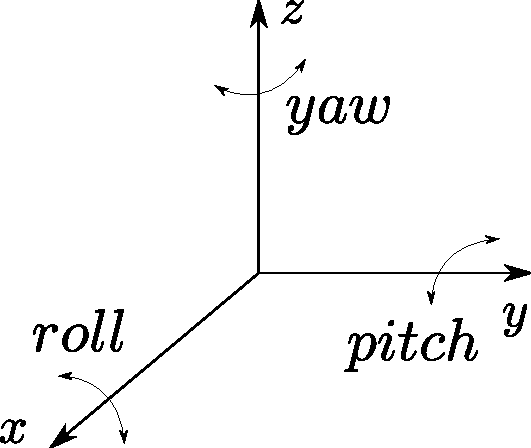
\includegraphics[width=0.3\textwidth]{graphics/roll_pitch_yaw.pdf}
	\caption{Roll-Pitch-Yaw-Winkel \cite{rollPitchYaw}}
	\label{fig:roll_pitch_yaw}
\end{wrapfigure}	%\end{figure}

Die Berechnung einer neuen Trajektorie wird durchgeführt, sobald neue Daten vom Modul \lstinline{HumanPosition} vorliegen.
Als $start$-Punkt wird dabei die aktuelle Roboterposition verwendet.
$next$ ist eine Roboter-Pose, die sich im Abstand $d_{hum}$ vor dem Menschen auf dem Vektor Roboter-Mensch befindet.
Im Abstand $d_{hum}$ vor der geschätzten zukünftigen Mensch-Position auf dem Vektor next-estimated befindet sich der dritte Punkt der Trajektorie: $following$.
Der Abstand $d_{hum}$ zum Menschen kann dabei als externer Parameter vorgegeben werden, der Wert beträgt standardmäßig $1,75m$.
In Abb. \ref{fig:trajektorie} wird dies in einer Schemazeichnung dargestellt.

\begin{figure}[h]
	\center
	% Trajektorien-Punkte der Bahnplanung
% Author : Tobias Roth

\newcommand\Punkt{\tikz[scale=0.07]\draw[thick](-1,-1)--(1,1)(-1,1)--(1,-1);} 

\begin{tikzpicture}


\def \dHum {1.5}

% Definition der Koordinaten für Roboter, Mensch_act und Mensch_est
\def \rX {0}
\def \rY {0}
\def \hActX {3}
\def \hActY {4}
\def \hEstX {8}
\def \hEstY {4}

% Setzen der Koordinaten für Roboter, Mensch_act und Mensch_est
\coordinate (r) at (\rX,\rY);
\coordinate (hact) at (\hActX,\hActY);
\coordinate (hest) at (\hEstX,\hEstY);

% Berechnung der Trajektorien-Punkte
\coordinate (trajPointA) at (r);
\coordinate (trajPointB) at (2.1, 2.8);	% hart codiert..
\coordinate (trajPointC) at (6.53095, 3.70137);	% hart codiert..

% Poitionen zeichnen
\node at (r) (R) {\Punkt};
\node[scale=0.9] at (r) [anchor=east] {$R$};
\node at (hact) (H_act) {\Punkt};
\node[scale=0.9] at (hact) [anchor=south east] {$H_{act}$};
\node at (hest) (H_est) {\Punkt};
\node[scale=0.9] at (hest) [anchor=south west] {$H_{est}$};

\node[scale=0.9] at (r) [anchor=west] {$A$};
\node at (trajPointB) (B) {\Punkt};
\node[scale=0.9] at (trajPointB) [anchor=north] {$B$};
\node at (trajPointC) (C) {\Punkt};
\node[scale=0.9] at (trajPointC) [anchor=north] {$C$};

% Vektoren zwischen Positionen
\path[name path global=rHact, -] (r) edge (hact);
\path[-] (hact) edge (hest);

% d_{Hum} zeichnen
\draw [name path global=hactCircle] (hact) circle (\dHum);
\draw [name path global=hestCircle] (hest) circle (\dHum);
\path[<->] (hact) edge node {$d_{hum}$} (\hActX,\hActY + \dHum);
\path[<->] (hest) edge node {$d_{hum}$} (\hEstX,\hEstY + \dHum);

% Eigentliche Trajektorie zeichnen
\path[red, thick, ->] (trajPointA) edge (trajPointB);
\path[red, thick, ->] (trajPointB) edge (trajPointC);



% Eigentliche Trajektorie zeichnen
% \path [name intersections={of=rHact and hactCircle, by={A}}];
% \node at (A) [below] {$A$};
% \path [name intersections={of=hactCircle and rHact}];
% \coordinate [label=above:$C$] (C) at (intersection-0);


\end{tikzpicture}

	\caption{Berechnung der Trajektorien-Punkte}
	\label{fig:trajektorie}
\end{figure}

Der $yaw$-Wert wird so berechnet, dass der Roboter sich immer in Richtung des Menschen ausrichtet.
So kann gewährleistet werden, dass die Kinect den Menschen weiterhin im Fokus hat.


% \begin{itemize}
% 	\item Modul bekommt aktuelle und geschätzte Position des Menschen, sowie aktuelle Position des Roboters
% 	\item Struktur der zu berechnenden Trajektorie duch \lstinline{OmniDriveAlongPath} \todoprivate{ref zu LowLevel?}\ vorgegeben:
% 	\begin{itemize}
% 		\item Start $(x,y)$, Koordinaten
% 		\item Following $(x,y,yaw)$, Koordinaten und Orientierung \todoprivate{Skizze zu x-y-z-roll-pitch-yaw ?}
% 		\item Next $(x,y)$, Koordinaten
% 	\end{itemize}
% 	\item Berechnung einer neuen Trajektorie, sobald neue Mensch-Daten vorliegen
% 	\item Berechnung der Trajektorien-Punkte im Einzelnen:
% 	\begin{itemize}
% 	  \item Start: aktuelle Roboterposition
% 	  \item Next: Pose auf Roboter-Mensch-Vektor, die sich im Abstand $d$ vor dem Mensch befindet; yaw wird gesondert berechnet, sodass Roboter immer zu Mensch schaut
% 	  \item Following: Position auf next-estimated-Vektor, die sich $d$ vor geschätzter Mensch-Position befindet
% 	  \item erfolgt alles in absoluten Weltkoordinaten
%   \end{itemize}
%   \item Parameter $d$ für den Abstand des Roboters zum Menschen, default: $1,75m$
%   \item Berechnung des yaw-Wertes: \todoprivate{Formel dazu}

% 	\item MUX für Trajektorie
% 	\begin{itemize}
% 		\item GenerateTrajectory
% 		\item LoadFromFile
% 	\end{itemize}
% \end{itemize}


\subsubsection{Pfadspeichern und -laden}
\label{bahnplanung_pfadSpeichernLaden_subsubsec}

% \begin{itemize}
%   \item Im \lstinline{followPerson} -Zustand: Wegpunkte $(x,y,yaw)$ werden in gewissen Abständen $d_{save}$ gespeichert
%   \begin{itemize}
%     \item sobald $ \overline{ s_{act} - s_{last} } > d_{save} $ \todoprivate{Fehler im Code??? Euklidischer Abstand stattdessen verwenden?}
%   \end{itemize}
% 	\item Im \lstinline{loadPath} -Zustand: Nächster Wegpunkt wird geladen, sobald vorheriger erreicht wurde
%   \begin{itemize}
% 		\item Im \lstinline{returnHome} -Zustand: Nächster Wegpunkt wird geladen, sobald vorheriger erreicht wurde; umgekehrte Reihenfolge
%     \item sobald $ d( s_{foll} - s_{act} ) < d( s_{nxt} - s_{act} ) $, Euklidischer Abstand
%   	\item \lstinline{yaw} wird unabhängig von Datei berechnet, sodass Roboter immer Menschen anschaut
%   \end{itemize}
%   \item Eigene Klasse zum File-Handling: \lstinline{fileUtil}
%   \begin{itemize}
%     \item Mehrere dump-files möglich
%     \item Auslesen der Wegpunkte in normaler und umgekehrter Reihenfolge
%   \end{itemize}
% \end{itemize}

Zur Pfadspeicherung bzw. zum Laden eines abgespeicherten Pfades werden zwei Module, sowie eine Helfer-Klasse verwendet:
\begin{itemize}
	\item \lstinline{StoreRoboterPositionsToFile}: Während dem Modus \lstinline{followPerson} (s. Abs. \ref{umsetzung_integration_sec} für weitere Informationen zur globalen Zustandsmaschine) aktiv\todoprivate{evtl. ref noch auf subsec}
	\item \lstinline{LoadRoboterPositionsFromFile}: Während dem Modus Während dem Modus \lstinline{followPath} (s. Abs. \ref{umsetzung_integration_sec}) aktiv\todoprivate{evtl. ref noch auf subsec}
	\item \lstinline{fileUtil}
\end{itemize}

Im globalen Modus \lstinline{followPerson} (s. Abs. \ref{umsetzung_integration_sec}\todoprivate{evtl. ref noch auf subsec}), also während dem Einlernen eines neuen Pfades, schreibt das Modul \lstinline{StoreRoboterPositionsToFile} in regelmäßigen Abständen $d_{save}$ Roboterposen in eine externe Datei (sog. \lstinline{dumpFile}).
Für die Posen werden dabei sowohl die $x$- und $y$-Koordinaten, als auch die $yaw$-Werte abgespeichert.
Der Zeitpunkt für die Abspeicherung der nächsten Pose wird anhand des euklidischen Abstands festgelegt:
Sobald der Abstand der aktuellen Roboterpose zur letzten Speicherpose größer als der Speicherabstand $d_{save}$ ist, wird die aktuelle Pose abgespeichert.
$d_{save}$ kann als Parameter in einer externen Konfigurationsdatei definiert werden.
\begin{equation}
	\| s_{act} - s_{last}\|_2 \quad > \quad d_{save}
\end{equation}

Innerhalb des \lstinline{dumpFile}s werden die $x$, $y$ bzw. $yaw$-Werte durch Doppelpunkte abgetrennt gespeichert.
Eine beispielhafter abgespeicherter Pfad ist in Listing \ref{lst:dump_file} dargestellt.
\todoprivate{Beispiel-Ausschnitt aus dump-file}
\begin{lstlisting}[caption=Beispiel für ein \lstinline{dumpFile} zur Speicherung eines Pfades, label=lst:dump_file]
	1111:2222:3333
	999:888.8:77.77
\end{lstlisting}

Im globalen Modus \lstinline{loadPath} (s. Abs. \ref{umsetzung_integration_sec}\todoprivate{evtl. ref noch auf subsec}), also während dem Abfahren eines gespeicherten Pfades, liest das Modul \lstinline{LoadRoboterPositionsFromFile} die Punkte aus dem \lstinline{dumpFile}.
Der euklidische Abstand findet wieder Verwendung, um den Zeitpunkt festzulegen, an welchem der nächste Punkt in die Trajektorie aufgenommen wird.
Dies geschieht, sobald der Abstand des Roboters zu $following$ kleiner ist als der zu $next$:
\begin{equation}
	\| s_{foll} - s_{act} \|_2 \quad < \quad \| s_{next} - s_{act} \|_2
\end{equation}
Im Modus \lstinline{returnHome} werden die Punkte in umgekehrter Reihenfolge ausgegeben.

In der aktuellen Implementierung werden die aus dem \lstinline{dumpFile} gelesenen $yaw$-Werte \emph{nicht} für die Trajektorie verwendet.
Grund hierfür ist die Entscheidung, dass der Roboter (bzw. die darauf installierte Kinect) immer den Menschen im Fokus behalten soll, um evtl. kurzfristige Stop-Kommandos empfangen und umsetzen zu können.
Die $yaw$-Werte, die während des Pfad-Einlernens abgespeichert wurden, beziehen sich auf die Standpunkte des Menschen zum dortigen Zeitpunkt, und nicht auf die aktuell relevanten Mensch-Positionen. 
Aus diesem Grund werden die $yaw$-Werte innerhalb des \lstinline{LoadRoboterPositionsFromFile}-Moduls auf Basis der aktuellen Mensch-Position gesondert berechnet.

Für die Aufgaben des Datei-Handlings wurde eine eigene Klasse implementiert, die Operationen wie Datei anlegen, öffnen, schließen, in die Datei schreiben, aus der Datei lesen etc. kapselt.
Hier werden die Daten aus der Datei gepuffert, sodass beispielsweise im Fall des Pfad-Lesens nur ein einmaliger Dateizugriff auf Betriebssystem-Ebene erfolgt.
Es ist auch möglich, mehrere \lstinline{dumpFile}s anzulegen.


% 
% % -----------------------------------------------------------------------------
% %													Transformationen
% \subsection{Transformationen}
% \label{transformationen_subsec}
% 
% \authorsection{\editorjulian}
% \todo[inline]{Julian: Sollen wir (also du ;-) ) noch so einen Abschnitt machen?}



% -----------------------------------------------------------------------------
%													Kollisionsvermeidung
\subsection{Kollisionsvermeidung}
\label{kollisionsvermeidung_subsec}

\subsubsection{Modul}
\authorsection{\editortobias}

% \begin{itemize}
%   \item Kollisionsvermeidungsmodul (\lstinline{ObstacleAvoidance}) überprüft die geplante Trajektorie auf Hindernisse, und plant ggf. um Hindernisse
%   \item Ausgaben von \lstinline{GenerateTrajectory} und \lstinline{LoadFromFile} werden geMUXt
%   \begin{itemize}
%     \item je nach Modus (\lstinline{followPerson} bzw. \lstinline{returnHome} / \lstinline{followPath}) schaltet MUX andere Eingänge durch
%   	\item Die Ausgabe des MUX wird dann widerum komplett durch das Kollisionsvermeidungsmodul (\lstinline{ObstacleAvoidance}) geschleift
%     \item Dadurch wird jede Trajektorie auf Hindernisse überprüft, keine kommt \glqq daran vorbei\grqq
%   \end{itemize}
%   \item Innerhalb des Moduls wird jede Trajektorie auf Hindernisse überprüft
% 	\begin{itemize}
% 	  \item die (Bild-)Punkte zwischen start, next und following werden berechnet (Transformation der Welt- in Bildkoordinaten)
% 	  \item Überprüfung für jeden einzelnen Punkt, ob er innerhalb eines Hindernisses liegt
% 	  \item Verwendung der \lstinline{ObstacleMap} \todoprivate{ref zu Lokalisierung}
% 	\end{itemize}
%   \item Ohne Hindernis werden Trajektorien-Punkte nur durchgeschleift
%   \item Wenn Hindernis erkannt, dann wird eine neue Trajektorie ermittelt
%   \begin{itemize}
%     \item Verwendung des A*-Algorithmus
%     \item Ermittlung des Start- und Endpunktes für A*
%     \item ggf. gesonderte Behandlung für Endpunkt (\lstinline{choosePointAfterObstacle})
%     \item Aufruf A*
%     \item Transformation der nuen Trajektorie IK $\rightarrow$ WK
%   \end{itemize}
% \end{itemize}

Das Modul \lstinline{ObstacleAvoidance} überprüft die geplante Trajektorie auf Hindernisse, und plant ggf. um ein Hindernis herum, um Kolissionen zu vermeiden.
Jede von \lstinline{GenerateTrajectory} bzw. \lstinline{LoadRoboterPositionsFromFile} (s. Abs. \ref{bahnplanung_trajektorie_subsubsec}) ausgegebene Trajektorie wird innerhalb des Moduls \lstinline{ObstacleAvoidance} auf Hindernisse überprüft, bevor sie an tiefer liegende Schichten weiter gegeben wird.
Dies wird durch einen \gls{mux} erreicht, der je nach globalem Modus die entsprechenden Eingänge an das Modul \lstinline{ObstacleAvoidance} durchschaltet.
So wird sichergestellt, dass ungeprüfte Trajektorien nicht an die Motoransteuerung weiter gegeben werden.
In Abb. \ref{fig:behaviours} (S. \pageref{fig:behaviours}) ist das Modul innerhalb der \lstinline{Behaviours}-Gruppe sichtbar.

Für die Hindernis-Überprüfung innerhalb des Moduls werden die Trajektorienpunkte, die alle in \gls{wk} vorliegen, in \gls{bk} transformiert.
So werden $start$, $next$ und $following$ auf entsprechende Punkte der \lstinline{ObstacleMap} (s. Abs. \ref{hinderniskarte_subsec}, S: \pageref{hinderniskarte_subsec}) abgebildet.
In einem weiteren Schritt werden alle \glstext{bk}, die zwischen den drei Trajektorienpunkten liegen, berechnet und in eine Liste geschrieben.
Die Punkte dieser Liste werden anschließend anhand der \lstinline{ObstacleMap} auf Hindernisse überprüft.

Falls für keinen der Punkte ein Hindernis festgestellt werden konnte, wird die Trajektorie (in \gls{wk}) unverändert weiter gegeben.

Liegt jedoch mindestens einer der Punkte innerhalb eines Hindernisses, so wird eine neue Trajektorie ermittelt, die um das Hindernis plant.
Hierfür wird der A*-Algorithmus verwendet.
Dieser benötigt einen Start- und einen Endpunkt, welche nicht innerhalb eines Hindernisses und auch nicht außerhalb des Bildes (\lstinline{ObstacleMap}) liegen dürfen.
Die Implementierung dieses Algorithmus wird im nächsten Abschnitt beschrieben.

Schließlich wird die durch den A*-Algorithmus neu berechnete Trajektorie in \gls{wk} umgerechnet, und an die Gruppe \lstinline{SegwayOmniReflexes} weiter gegeben.



\subsubsection{Algorithmus}
\authorsection{\editorjulian}
\todo[inline]{Julian: Schreiben}

Um einen kollisionsfreien Pfad zu erstellen kommt eine Bahnplanungsmethode zum Einsatz, die den A*-Algorithmus verwendet. Um den zeitlichen Aufwand einer eigenen Implementierung zu vermeiden wurde auf eine bereits existierende und frei verfügbare Implementierung von Justin Heyes-Jones zurückgegriffen.
\todoprivate{Website und ref angeben}
Diese Implementierung kann einfach eingebunden und erweitert werden. Zum Einbinden des Algorithmus sind drei wesentliche Änderungen bzw. Erweiterungen notwendig:
\begin{description}
	\item[Hinderniskarte] Eine Schnittstelle zur Verwendung eines \lstinline{CByteImage} als Hinderniskarte.
	\item[Heuristik] Ersetzen der ursprünglichen Heuristik durch die Euler-Distanz.
	\item[Antigravitationsfeld] Erweiterung um ein Antigravitationsfeld.
\end{description}

Um beliebige Datencontainer als Hinderniskarte verwenden zu können wurde eine Interface-Klasse geschaffen. Bei deren Umsetzung muss eine Funktion implementiert werden die für eine Koordinate auf der Hinderniskarte die Information liefert ob sich dort ein Hindernis befindet oder nicht. Eine entsprechende Implementierung wurde sowohl für ein \lstinline{CByteImage} als auch für ein \lstinline{IplImage} vorgenommen.

In der ursprünglichen Implementierung wurde die Manhattan-Distanz zwischen zwei Punkten als Heuristik für den A*-Algorithmus verwendet. Da sich der Roboter omnidirektional bewegen kann ist es sinnvoll stattdessen die Euler-Distanz zu verwenden.
\todo[inline]{eventuell noch eine Fußnote dazu?}

\begin{figure}[h]
	\centering
	\label{fig:bahnplanung_umsetzung_algorithm}
	\subfloat[Ursrpüngliche Hinderniskarte]
	{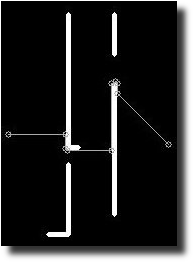
\includegraphics[scale=0.8]{graphics/BILD-Astar_normale_hindernisse.png}}
	\quad
	\subfloat[Hinderniskarte mit großen Hindernissen]
	{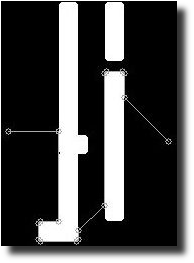
\includegraphics[scale=0.8]{graphics/BILD-Astar_grosse_hindernisse.png}}
	\quad
	\subfloat[Hinderniskarte mit Antigravitationsfeld]
	{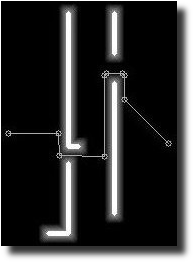
\includegraphics[scale=0.8]{graphics/BILD-Astar_antigrav.png}}
	\caption{Darstellung der Hinderniskarte und der gefundenen Trajektorie mit Hilfe des A*-Algorithmus, mit vergrößerten Hindernissen und mit Antigravitationsfeld.}
\end{figure}


%\begin{figure}[h]
%  \centering
%  \subfloat[Geplante Umgebung]{\label{fig:map_fzi_plan}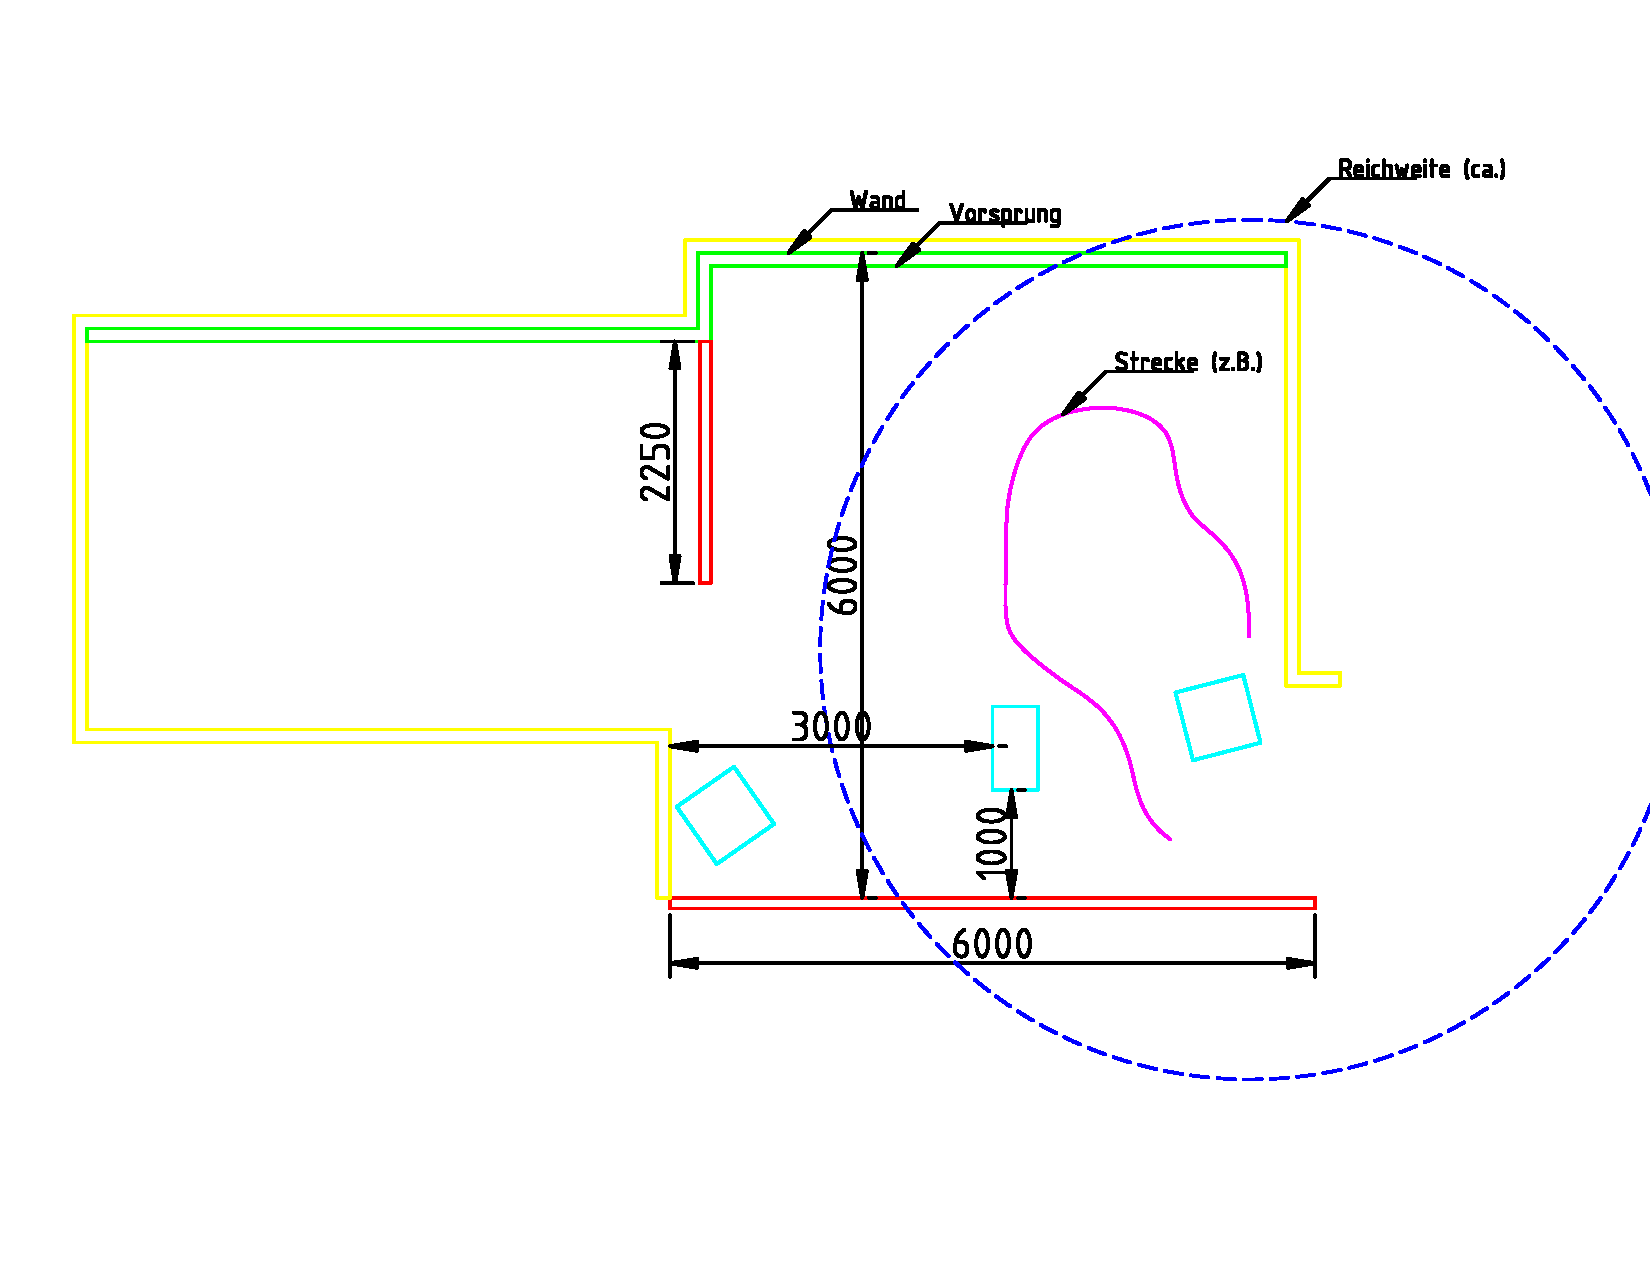
\includegraphics[width=0.45\textwidth]{graphics/map_fzi_plan}}
%  \quad %add desired spacing between images, e. g. ~, \quad, \qquad etc. (or a blank line to force the subfig onto a new line)
%  \subfloat[Umgebung mit \protect\gls{hollie} und realen Scannerdaten]{\label{fig:map_fzi_hollie}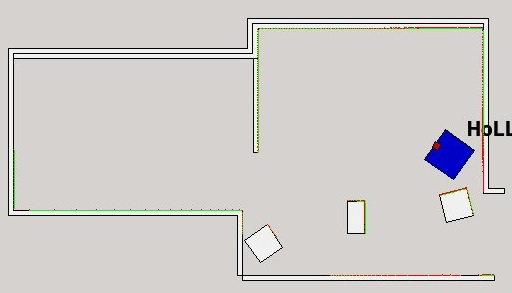
\includegraphics[width=0.4\textwidth]{graphics/map_fzi}}
%  \caption{Simulierte Büroumgebung für weitere Tests}
%  \label{fig:map_fzi}
%\end{figure}

In der Praxis stellte sich bei der Verwendung des A*-Algorithmus heraus, dass die verwendete Implementierung nicht den optimalen, also kürzesten Weg, findet und sich an Hindernissen entlang bewegt. Dieses Verhalten führte bereits in der Simulation zu erheblichen Problemen, konnte allerdings durch die Erweiterung um ein Antigravitationsfeld abgemildert werden.

Um einen gewissen Abstand zu Hindernissen einzuhalten sind zwei Lösungen denkbar. Die einfachste Variante ist es die Hindernisse in der Hinderniskarte \glqq aufzublasen\grqq\ und so in der Realität für einen Mindestabstand zu sorgen. Alternativ gibt es die Möglichkeit ein Antigravitationsfeld einzusetzen. 

Beim einfachen Vergrößern der Hindernisse kommt es an Passagen bei denen der Roboter, in der ursprünglichen Hinderniskarte, wenig Platz auf beiden Seiten hat, zum Verschluss dieser Durchgänge. Dies kann beispielsweise bei Türen der Fall sein. Das Finden eines kollisionsfreien Pfades ist unmöglich, da die Passage nunmehr ein Hindernis ist. Um diesem Problem zu begegnen kommt die zweite Lösungsmöglichkeit zur Verwendung. Das Antigravitationsfeld wird realisiert in dem das Fahren in der Nähe von Hindernissen mit Kosten verbunden ist. Konkret erfolgt die Realisierung durch das Belegen der Pixel mit Grauwerten, welche die Kosten repräsentieren die es benötigt um \glqq auf\grqq\ diesen Pixel zu fahren. Der Algorithmus versucht den günstigsten Weg zu finden und vermeidet das fahren auf \glqq teueren\grqq\ Pixeln. Da es aber erlaubt ist auf diesen Pixeln zu fahren kann ein kollisionsfreier Pfad auch durch enge Passagen gefunden werden.



% -----------------------------------------------------------------------------
%													Simulation
\subsection{Simulation}
\label{simulation_subsec}
\authorsection{\editoroier}

Für die Simulation war schon eine Simulationsumgebung vorhanden.
Aufgabe war es, eine grafische Oberfläche mit Mcagui zu erstellen.
Warum ist die Simulation nützlich oder notwendig?
In erster Linie konnte man am Anfang am realen Roboter nicht testen, weil der Roboter noch gebaut wurde oder zum Beispiel nicht alle von uns programmierten Komponenten (wie bspw. die Lokalisierung) funktionsfähig waren.
Dank der Simulation wurde das Testen von einzelnen Funktionalitäten und die Darstellung des Roboterzustands möglich, wie man in Abbildung \ref{fig:mcagui} sehen kann.
\ZB wurde die Simulation sehr oft benutzt, um schnell Änderungen im Bahnplanungsalgorithmus zu testen.

\begin{figure}[h]
\centering
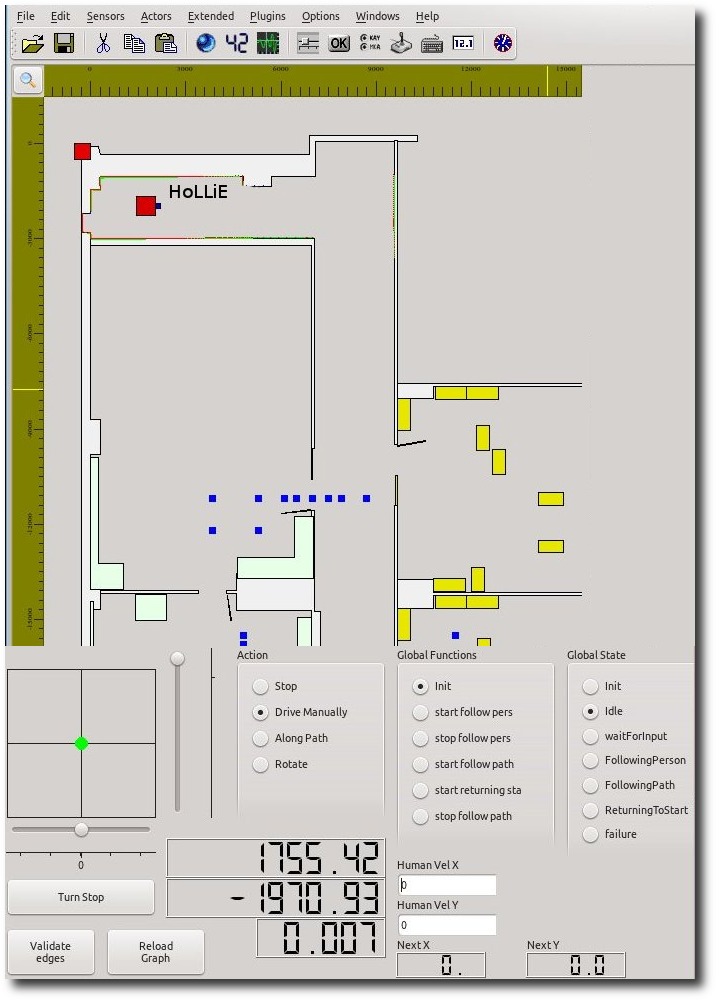
\includegraphics[scale=0.4]{graphics/mcagui_screenshot.png}		
\caption{\label{fig:mcagui} Die entwickelte Simulationsoberfläche
}
\end{figure}

Ein Problem am Anfang war, wie man den zu verfolgenden Menschen simulieren sollte.
Um dies zu lösen, benutzt man einfach Mausklicks auf der Karte.

% #############################################################################
%															Hinderniskarte und Lokalisierung
% #############################################################################
\chapter{Hinderniskarte und Lokalisierung}
\label{lokalisierung_cha}
% ********************************************************************************
% 										Aufgabenstellung
% ********************************************************************************
\section{Aufgabenstellung}
\label{lokalisierung_aufgabenstellung_sec}
\authorsection{\editorandreas}
% -----------------------------------------------------------------------------
%													Lokalisierung
\subsection{Lokalisierung}
Die Aufgabe der Lokalisierung, im Kontext der Robotik, ist die Bestimmung der
Roboter Pose, welche die Position und Orientierung des Roboters in seiner Umgebung vollständig beschreibt.
 Um Bahnplanung und Steuerung zu ermöglichen muss die Pose des Roboters bekannt sein,
 damit sich dieser gefahrlos fortbewegen und sicher mit der Umwelt interagieren kann.
 Für einen Menschen ist die Lokalisierung selbstverständlich, für einen Roboter
 stellt sie allerdings eine Herausforderung dar.
 Aufgrund einer unbekannter Startposition oder von Messungenauigkeiten während
 der Fortbewegung kann die Pose eines Roboters nur in den seltensten Fällen genau bestimmt werden. Für eine Lokalisierung wird weiterhin eine Karte der Umgebung benötigt,
 da ohne diese die Pose nicht bestimmte werden kann. Von lokaler Lokalisierung wird gesprochen wenn die aktuelle Pose des Roboters
 in seiner Umwelt bekannt ist und sie bei einer Bewegung des Roboters
 fortlaufend aktualisiert wird um sie auf dem neusten Stand zu halten. Hier
 werden Schätzungen der Bewegung aufgrund der Odometrie Sensorik mit Hilfe von weiteren Daten zur Posenbestimmung korrigiert. Dieses Vorgehen soll eine Aufsummierung von Fehlern bei der
 Schätzung der Bewegung durch die Odometrie verhindern. Im Gegensatz dazu ist
 bei der globalen Lokalisierung die aktuelle Pose des Roboters in seiner Umwelt
 nicht bekannt und muss zum Beispiel anhand von Kartenmaterial geschätzt werden.
 Man sieht leicht ein, dass bei dieser Art der Lokalisierung die Initiale
 Schätzung einen beliebig großen Fehler aufweisen kann. Wie wir gesehen haben
 ist es also notwendig eine Lokalisierung durchzuführen um es unserem Roboter zu
 ermöglichen sich fortzubewegen.
% -----------------------------------------------------------------------------
%													Hinderniskarte
\subsection{Hinderniskarte}
Abgesehen von der Lokalisierung gibt es noch einen weiteren Grund warum es für einen mobilen Roboter unumgänglich ist,
 dass eine interne Repräsentation seiner Umgebung existiert. Karten, die zur Lokalisierung eingesetzt werden,
 enthalten meist nicht alle statischen Hindernisse, da diese Karten zu einem gewissen Zeitpunkt erstellt wurden und
 in der Zwischenzeit wahrscheinlich neue Objekte hinzugekommen oder bereits Vorhandene versetzt worden sind.
 Außerdem enthalten solche Karten offensichtlich keine Hindernisse die sich bewegen können, wie beispielsweise Menschen.
 Ein Hindernis ist ganz allgemein ein Bereich der von dem Roboter nicht befahren werden kann. Eine Darstellung der Hindernisse
 relativ zur Roboterpose wird als Hinderniskarte bezeichnet. Eine solche Karte
 kann zum Beispiel mit Hilfe von Laser- oder Kameradaten erstellt werden.
 Eine Kombination des Materials mehrerer Sensoren ist normalerweise das Sinnvollste,
 da Laser beispielsweise keine negativen Hindernisse erkennen können.
 Als negative Hindernisse werden Bereiche bezeichnet die im Vergleich zur
 gegenwärtigen Position eine geringere Höhe aufweisen.
 Ein Beispiel für ein solches Hindernis ist eine Treppe in ein tiefer gelegenes
 Stockwerk. Das erstellen einer Hinderniskarte ist aus den oben genannten
 Gründen essentiell um eine Bahnplanung für einen mobilen Roboter durchzuführen.
% -----------------------------------------------------------------------------
%													Virtual protective Field
\subsection{Virtual protective Field}
Die Aufgabe der Bahnplanung besteht darin auf Grundlage der Lokalisierung und der Hinderniskarte einen Weg zu einer
 bestimmten Position zu finden. Danach wird dieser Weg vom Roboter abgefahren. Allerdings kann es während dem Abfahren der gefundenen
 Route Aufgrund eines Hindernisses, dass sich in den Weg des Roboters bewegt bevor erneut geplant werden kann oder
 schlicht Aufgrund eines Fehlers in der Planung dazu kommen, dass der Roboter mit einem Hindernis kollidiert.
 Daher wird eine Möglichkeit benötigt auf einer tieferen Ebene wie der Bahnplanung das unbeabsichtigte kollidieren mit einem Hindernis
 zu verhindern. An dieser Stelle kommt das sogenannte „Virtual protective Field“ ins Spiel, von welchem ein Bereich um den Roboter auf
 Hindernisse überprüft und beim Auffinden eines Solchen ein Signal erzeugt wird, damit der Roboter gestoppt werden kann bevor er
 auf das Hindernis trifft. Dieser Bereich muss mit der Geschwindigkeit des
 Roboters wachsen bzw. schrumpfen so das sichergestellt ist, dass auf jeden
 Fall eine Kollision verhindert werden kann.
% ********************************************************************************
% 										Grundlagen Lokalisierung
% ********************************************************************************
\section{Grundlagen Hinderniskarte und Lokalisierung}
\label{lokalisierung_grundlagen_sec}
\authorsection{\editordummy}
\todo[inline]{Lokalisierungs-Gruppe: Schreiben}
% -----------------------------------------------------------------------------
%													Lokalisierung
\subsection{Lokalisierung}
\todo[inline]{Geplanter Aufbau -> Theorie, kurze Beschreibung der Vorhandenen
und zur Umsetzung verwendbaren Gruppe und Module}
 Odometrie

Ein einfacher Ansatz zur Positionsbestimmung ist die Verwendung von Schrittzählern, welche die Bewegung der Roboterräder oder -Beine misst. Über eine Umrechnungsfunktion (meist: lineare Abbildung) lässt sich aus der Anzahl der zurückgelegten Schritte eine Pose relativ zur Ausgangspose berechnen.
Vorteile

    Relativ Stör-unanfällig unter Normalbedingungen (Ausnahmen: glatter, weicher, unebener Untergrund)
    Vernachlässigbarer Rechenaufwand
    Vernachlässigbarer Implementations-Aufwand 

Nachteile ¶

    Offset-Fehler steigt linear mit dem Betrag der Schrittzahl
    Ursprungsposition muss bekannt sein (vorgegeben werden)
    Fehler abhängig vom Untergrund
    Bei auf Schlupf basierenden (omnidirektionalen) Plattformen Fehler höher 
    
Kartenbasierte Lokalisierung

Anhand von gegebenem Kartenmaterial kann aus einem Sensorbild der Umgebung die Position des Roboter geschätzt werden. Dazu werden zum Beispiel markante Punkte aus dem Sensorbild mit den Daten des Kartenmaterials abgeglichen. Im bestmöglichen Fall existiert nur eine mögliche Übereinstimmung, anhand derer der Roboter seine eigene Position bestimmen kann.
Vorteile

    Keine Fehlerakkumulation über Zeitverlauf
    Keine Ursprungsposition notwendig 

Nachteile

    Störanfällig (spiegelnde Oberflächen, bewegende Objekte)
    Benötigt aktuelles Kartenmaterial
    hoher Rechenaufwand
    hoher Implementierungs-Aufwand 
    
Landmarkbasierte Lokalisierung

In einer bekannten Umgebung können Landmarks (QR-Codes, Bodenlinien, GPS-Satelliten) angebracht werden. Diese können durch Sensoren am Roboter wiedererkannt werden und ermöglichen die Lokalisierung z.B. mittels Triangulierung.
Vorteile

    Fehler niedrig (durchschnittlicher Fehler niedrig)
    Keine Fehlerakkumulation über Zeitverlauf
    Zuverlässig (max. Fehler niedrig) 

Nachteile

    Landmarks notwendig
    Landmarks müssen von überall sichtbar sein
    Kartenmaterial u.U. notwendig 
    
Kombination der Messverfahren

Um die Nachteile der verschiedenen Lokalisierungsmethoden zu verringern werden in der Regel mindestens zwei Methoden miteinander kombiniert. Aufgrund der einfachen Implementierung und der geringen Störanfälligkeit ist meistens die Odometrie in Kombination mit anderen Systemen vorzufinden. Bei Verwendung mehrerer Methoden sind dementsprechend viele fehlerbehaftete Annahmen der aktuellen Roboterpose gegeben. Aus diesen Annahmen wird bestmöglichst die aktuelle Roboterpose bestimmt. Ein Verfahren, um den gesamten Fehler zu minimieren ist das Kalman-Filter. 
 Das Kalman-Filter

    TODO: Kurze Erläuterung / Einführung in das Kalman-Filter

% -----------------------------------------------------------------------------
%													Hinderniskarte
\subsection{Hinderniskarte}
\todo[inline]{Geplanter Aufbau -> Theorie, kurze Beschreibung der Vorhandenen
und zur Umsetzung verwendbaren Gruppe und Module}
Keine Hinderniskarte vorhanden
% -----------------------------------------------------------------------------
%													Virtual protective Field
\subsection{Virtual protective Field}
\todo[inline]{Geplanter Aufbau -> Theorie, kurze Beschreibung der Vorhandenen
und zur Umsetzung verwendbaren Gruppe und Module}
Virtual Protective Field lediglich für Differentialantrieb implementiert

% ********************************************************************************
% 										Umsetzung
% ********************************************************************************
\section{Umsetzung}
\label{lokalisierung_umsetzung_sec}
\authorsection{\editordummy}

% -----------------------------------------------------------------------------
%													Lokalisierung
\subsection{Lokalisierung}
\todo[inline]{Geplanter Aufbau -> Grundlegende Idee für die Umsetzung, Bild der
Gruppe, erläutern der Funktion der Module} Vorhandene Implementierung der
Lokalisierung anhand von Odometrie und Laserdaten im Odete-Projekt
Hardware Abstraction Layer (Hal) und (später) Scanner Abstraction Layer (Sal)
aus dem bereits bestehenden Segway Omni Projekt

Übernahme der MCA2-Struktur zur Lokalisierung von Odete

Adaption der Vorhanden Gruppen und Module zur Lokalisierung 
Anpassung von LLSP, HLSP, Hal \& Sal an das Segway Omni Projekt
Erweiterung auf beliebige Menge von Scannern
Einbindung eines PixelRemovers zur Wegnahme fehlerhafter Scanner-Pixel

% -----------------------------------------------------------------------------
%													Hinderniskarte
\subsection{Hinderniskarte}
\todo[inline]{Geplanter Aufbau -> Grundlegende Idee für die Umsetzung, Bild der
Gruppe, erläutern der Funktion der Module}

Erzeugung der Hindernisskarte aus den Laserdaten
Verwendung von Bildverarbeitungs-Modulen (SenseIVT)
            Gute Visualisierung
            Einfache Anpassung
            Verwendung von Standard-Filtern
         Repräsentation als Schwarz-Weiß-Bitmap
        Hindernisse auf den Radius des Roboters aufgebläht
        Anschließende Schließen Operation
% -----------------------------------------------------------------------------
%													Virtual protective Field
\subsection{Virtual protective Field}
\todo[inline]{Geplanter Aufbau -> Grundlegende Idee für die Umsetzung, Bild der
Gruppe, erläutern der Funktion der Module}
    Erstellen eines neuen Virtual Protective Fields aufgrund der Fähigkeit zur omnidirektionalen Bewegung
        Ausnutzen der bereits bestehenden Hindernisskarte
            Verwendung von Bildverarbeitungs-Modulen (SenseIVT)

Implementierung als Schwarz-Weiß-Bitmap

        3 unterschiedliche Virtual Protective Fields
            Sideward
            Forward
            Combined
        Dynamische Ausdehnung proportional zu (Geschwindigkeit)ins quadrat
        AND-Operation zwischen Hindernis- und Feldpixeln
        Ausgabe von Controller Output bei erkannten Hindernissen


\chapter{Tracking und Gestenerkennung}

\section{Aufgabenstellung}
\label{kinect_aufgabenstellung_sec}
\todo[inline]{Author hinzufügen}
\authorsection{\editordummy}

Die Kinect-Gruppe bekam die Aufgabe, durch Verarbeitung eines Video- und
 Tiefenbildes eine Person zu verfolgen und ihre speziellen
 Körperhaltungen/Gesten/Bewegungen als Kommandos zu interpretieren.
 Um die Bedürfnisse der anderen Gruppen zu erfüllen, mussten wir den Geschwindigkeitsvektor des verfolgten Menschen und die
 erkannte Geste als Ausgabewerte unseres Moduls weitergeben. Der Videostrom wurde von einem Kinect-Sensor akquiriert.
\vspace{0.3cm}

\noindent Output-Daten mit Nummerierung (\lstinline{openni_source_test SO}):
\begin{enumerate}[start=0]
  \item X-Position des Benutzers
  \item Y-Position des Benutzers
  \item Betrag der Benutzers Geschwindigkeit
  \item Richtung der Benutzers Geschwindigkeit
  \item X-Komponente des Geschwindigkeitsvektors
  \item Y-Komponente des Geschwindigkeitsvektors
  \item Erkannte Geste
  \item Benutzer anwesend
\end{enumerate}

\section{Grundlagen Kinect}
\label{kinect_grundlagen_sec}
\todo[inline]{Author hinzufügen}
\authorsection{\editordummy}

Sowohl die Bildqualität von Sensoren, als auch die Verarbeitungsalgorithmen zeigten eine erhebliche Entwicklung in den letzten Jahren.
 Heutzutage sind 3D-Entfernungskameras durch rapide Entwicklung des
 Entfernungsbildaufnahmeverfahren für breite Anwenderkreise erschwinglich
 (unter anderem Microsoft Kinect oder Asus Xtion PRO LIVE).
 Darum können neben 2D Farbbildern immer häufiger 3D-Bilder in Anspruch genommen
 werden. Bewährte Tatsache ist, dass Tiefenkarten eine viel robustere Darstellung geben, als herkömmliche Intensitätsbilder.
 
Im \gls{fzi}-Labor steht eine Kinect Kamera für die Datenakquirierung zur
 Verfügung, die ursprünglich als Zubehör der Microsoft XBOX 360 Spielkonsole
 entwickelt wurde. Der größte Vorteil dieses Sensors liegt in seinem Preis. Eine
 solche Kamera ist bereits für ca 100 Euro erhältlich und wird aufgrund dessen
 immer öfter verwendet.
 
Da die Kinect gleichzeitig sowohl 2D Farbbilder als auch 2.5D Entfernungsbilder liefert, gibt es die Möglichkeit, Verarbeitungsmethoden beliebig zu vermischen.
 Obwohl vielversprechend beschränkten wir uns, wegen hohen Rechenaufwandes, auf
 die Verarbeitung von 2.5D Bildern.
\vspace{0.3cm}

\subsection{Technische Daten}
\label{kinect_umsetzung_technische_daten}

\subsubsection{Tiefensensor}
\label{kinect_umsetzung_tiefensensor}

Dieser Sensor besteht aus der Kombination einer 830nm Laser Diode und einem Tiefensensor CMOS welcher die reflektierten Infrarotstrahlenempfangen kann. Aus der Laufzeit kann so die Tiefe der einzelnen Punkte berechnet werden.

\begin{itemize}
	\item Auflösung: 640x480 Pixels
	\item Tiefenbereich: 0.5m - 10m, Ideal 2m-2.5m
	\item Tiefengenauigkeit: 1cm
\end{itemize}

Ein Tiefenbild besteht somit aus 640x480 Pixeln mit je einer Tiefeninformation proPixel. Diese Tiefeninformation bewegt sich in einem Bereich von 50cm bis 1000cm mit einer Auflösung von 1cm. Pro Sekunde liefert der Kinect-Sensor 30 Tiefenbilder.

\subsubsection{Kamerasensor}

Neben dem Tiefensensor besitzt die Kinect eine normale RGB-Kamera. Diese löst mit 640x480 Pixeln auf.

\subsubsection{Audio}

Der Kinect-Sensor ist mit 4 Mikrofonen ausgestattet. Mit diesen ist eine 3D Lokalisierungmöglich. Der Zugriff auf die Audio-Daten ist jedoch noch mit keinem Framework möglich und es sind auch keine weiteren Informationen bekannt.

\subsubsection{Neigesteuerung}

Der Kinect-Sensor beinhaltet einen 3D-Neigesensor und einen Motor mit welchem der Neigungswinkel gegen vorne angepasst werden kann. Der Neigungswinkel beträgt zwischen $-31^\circ$und $+30^\circ$ relativ zum Standfuss.

\subsubsection{LED-Steuerung}

Das Integrierte LED kann ebenfalls angesteuert werden. Folgende Modus sind möglich:

\begin{itemize}
	\item LED-Ausgeschaltet
	\item Grün
	\item Rot
	\item Gelb (Orange)
	\item Gelb (Orange) blinkend
	\item Grün
	\item Gelb (Orange)-Rot blinkend
\end{itemize}

\noindent Die wichtigsten technischen der Kinect sind:
\begin{itemize}
  \item VGA-Auflösung (640x480 Pixel), weshalb die Bildqualität vergleichsweise
  schwach ist.
  \item Zur Entfernungsmessung verwendet die Kinect eine Infrarot TOF-Kamera und kodiert
  die Tiefenbilder durch 11 Binärzeichen (verteilt die maximale messbare
  Entfernung auf 2048 Teile). In dieser Auflösung liefert die Kinect 30 FPS.
\end{itemize}

Es existieren mehrere Schnittstellen um auf die Bilder zuzugreifen (OpenNI, OpenCV, Matlab, etc.).
 Unsere Wahl war OpenNI, weil wir sie durch C++ Umgebung in das
 \lstinline{MCA2}-Rahmenwerk einbinden konnten.

\subsection{OpenNI}

Mit OpenNI besteht ein Framework, welches unterschiedliche NUI (Natural User Interface) Geräte ansprechen kann, sofern dafür Treiber vorliegen. Das OpenNI-Framework stellt die Schnittstelle zwischen Anwendungssoftware und Treiber für einzelne NUI Geräte zur Verfügung. Daneben lässt sich das  Framework mit Middleware erweitern, um z.B. Skeleton Algorithmen einzubauen. Einer dieser Middleware Komponenten ist der Skeleton-Algorithmus NITE 1 von PrimeSense.

Das OpenNI-Framework ist in C++ geschrieben und steht für alle gängigen Plattformen (Windows, Linux/Ubuntu, OSX) zur Verfügung. Für Windows besteht zusätzlich ein Wrapper in C-Sharp.
Für den Softwareentwickler stehen die folgenden Komponenten des OpenNI-Frameworks im Vordergrund:

\begin{itemize}
	\item Context:  Definiert des Umfeld des Sensors. Dies Beinhaltet z.b. die Auflösung der Sensoren bzw. die Sicht auf die ganze Szene als solches.
	\item DepthGenerator:  Erzeugt für den Softwareentwickler ein kontinuierliches Signalwelches aus den Daten des Tiefensensors gespiesen wird.
	\item UserGenerator: Liefert Informationen zu aktuell erkannten Benutzern
\end{itemize}

Mit NITE  sind in OpenNI  User-Detection und -Tracking bereits einhalten. Auch einfache Gesten werden von der NITE-Middleware erkannt und können auf der Applikationsschicht direkt verwendet werden. Mit der NITE-Middleware kann OpenNI zudem so erweitert werden, dass zu einer erkannten Person die Gelenkpositionen errechnet werden.

Wir haben uns auf Grund des großen Funktionsumfangs und weiteren wichtigen Kriterien zur Verwendung dieses Frameworks entschieden.

\section{Umsetzung}
\label{kinect_umsetzung_sec}
\todo[inline]{Author hinzufügen}
\authorsection{\editordummy}

OpenNI ist eine Klassenbibliothek, die für die Programmierer einen einheitlichen Zugriff und Verarbeitungsmöglichkeiten
 der Sensordaten (Farbbild, Tiefenbild, Audiosignale) anbietet. Bei natürlicher Interaktion (NI steht für „natural interaction“) wird der Input,
 wie Handbewegungen, bestimmte Körperhaltungen, als Steuerungssignale für die Anwendung interpretiert. Die Systemstruktur OpenNIs ist modular.
 Mit dem entsprechenden (sensorspezifischen) Interface muss immer die generelle, wiederverwendbare Struktur ergänzt werden.
 Ein solches Interface und Treibersoftware für den Kinect-Sensor ist von Prime
 Sense erhältlich. 

OpenNI liefert eine eingebaute Segmentierung, die nach unserer Erfahrungen robust funktioniert.
 Anfangs muss nur eine bestimmte Kalibrierungspose eingenommen werden. Danach wird der Körper kontinuierlich segmentiert und
 auf dem Bildschirm mit einer Farbe gekennzeichnet. Der zugrunde liegenede Algorithmus ist gekapselt und war somit von uns nicht einsehbar.
 Der Ansatz das Modul zu verwenden schien eine gute Wahl zu sein.

Wie im vorigen Absatz erläutert werden Personen kontinuierlich segmentiert. Das
„NIUserTracker“ Programm liefert auch das Skelett aller kalibrierten und registrierten Personen. Das Gerüst enthält die Poseninformation über jedes
 Gelenk. Für unseren Ansatz waren Halsposition (\lstinline{XN_SKEL_NECK}), beide
 Ellenbogenpositionen (\lstinline{XN_SKEL_LEFT_ELBOW},
 \lstinline{XN_SKEL_RIGHT_ELBOW}), beide Schulterpositionen
 (\lstinline{XN_SKEL_LEFT_SHOULDER}, \lstinline{XN_SKEL_RIGHT_SHOULDER}), beide
 Hüftenwerte (\lstinline{XN_SKEL_LEFT_HIP}, \lstinline{XN_SKEL_RIGHT_HIP}) und
 die Positionen beider Handflächen (\lstinline{XN_SKEL_LEFT}\\\lstinline{_HAND},
 \lstinline{XN_SKEL_RIGHT_HAND}) relevant. Das Programm gibt außerdem
 Konfidenzwerte, d.h. Einschätzungen über die Güte von Messwerte, dieser Positionen zurück.
 Bei ausrechend hohen Konfidenzwerten (>50\%) verwendeten wir die gemessenen
 Poseninformationen in der weiteren Verarbeitung. Alleinig die Handgelenke/Handflächen bildeten eine Ausnahme,
 da deren Orientierungen (aus unbekanntem Anlass) stets schlechte Konfidenzwerte lieferten. Die relevnten Positionsmessungen der Hände waren jedoch gut.

Aus dem OpenNI-Modul importierten wir nur Tiefenbilder, um diese im
\lstinline{MCABrowser} anzuzeigen. Dazu wurde ein spezieller Datentyp,
„Blackboard“, verwendet (normalerweise können an den Kanten nur Double-Werte zwischen den Modulen weitergegeben werden).

Alle anderen Verarbeitungsprozesse wurden in die \lstinline{MCA2}-Umgebung,
durch die Verwendung von früher implementierten Modulen und Funktionen, integriert.

\begin{figure}[h]
\center
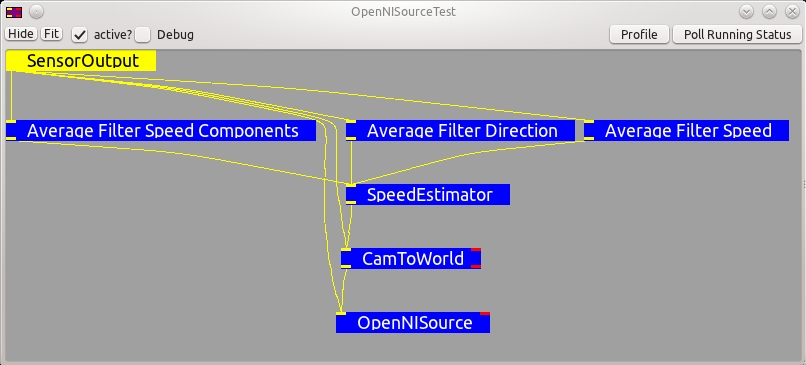
\includegraphics[scale=0.5]{graphics/OpenNISourceTest.jpg}
\caption{\label{fig:OpenNISourceTest} Die \lstinline{MCA2}-Grundstruktur
unseres Moduls in \lstinline{MCABrowser}}
\end{figure}

Zur Geschwindigkeitsschätzung wird der Torso (Rumpfmittelpunkt) auf den Boden projiziert
 (die Z-Koordinate – im Welt-Koordinatensystem - wird auf 0 gesetzt). Da die
 Positionsinformation wegen der hohen FPS-Rate mit viel Rauschen belastet wird
 (man bewegt sich langsam, die geringe Auflösung der Kinect aber interpretiert
 dies jedoch als geringfügige Posenänderungen im Ruhezustand.), muss die Positionveränderungen
 in größeren Zeitschritten ausgewertet werden. Dazu verwenden wir einen Glättungsfilter über
 je 5 Bilder (\lstinline{Average Filter Speed Components}, \lstinline{Average Filter Direction}, \lstinline{Average Filter Speed}).
 
Bevor die Geschwindigkeit für eine Abtastperiode aus der Differenz von den
aktuellen und vorherigen Werten kalkuliert wird (\lstinline{Speed Estimator}),
müssen die Koordinaten aus dem Kinect-Koordinatensystem in Roboterkoordinaten transformiert werden
 (\lstinline{CamToWorld}). Dieser Schritt benötigt die Kamerakalibration des
 Kinect-Sensors. Dies muss nur einmal gemacht werden, und kann mit OpenCV oder
 in MATLAB (Camera Calibration Toolbox) durchgeführt werden. Die Ergebnisse (die extrinsischen Parameter)
 sollen durch ein ``Init-File'' (``calibration\_data.txt'' genannt) für das
 Programm zur Verfügung stehen.
 Anhand dieser Datei stellt die Anwendung die ``Kamera zu Roboter'' Transformationswerte automatisch ein.
 
Noch eine wichtige Bemerkung zur Geschwindigkeitsberechnung: da die FPS-Rate
 sich kontinuierlich ändert, muss stets der aktuelle FPS-Wert eingeholt werden.
 Dazu wird eine Zeitmessung zwischen zwei Abtastwerten eingeholt.

Die Zeit wird in Sekunden, die Entfernungen und Bewegungen werden in Millimeter gemessen.
 Die verwendeten Einheiten sind mm (Position, Positionsveränderung), mm/sec
 (Geschwindigkeit), frame/sec (Frame-Rate) und rad (Winkel).

Die Gestenerkennung wurde in einem zweiten Modul (\lstinline{GestureClassifier})
umgesetzt, das in Laufzeit aus \lstinline{OpenNISource} aufgerufen wird.

\subsection{Gestenerkennung}

Ursprünglich sollte eine beliebig erweiterbare Struktur zur Gestenerkennung verwendet werden.
 Diesem Ansatz liegt ein binärer Entscheidungsbaum zu Grunde, dem den einzelnen
 Output-Mög"-lich"-kei"-ten (den Blätter des Baums, also den eigentlichen
 Gesten) Identifikationsnummern zugeordnet werden.

Diese Struktur bietet programmierungstechnisch eine generische Lösung. Sie funktioniert anatomisch universal,
 also unabhängig von konkreten Körpermaßen der Person, durch die Verwendung relativer Merkmale.
 Dies sind zum Beispiel Winkel zwischen bestimmten Körperteilen.
 
Aufgrund der groben Auflösung und der stark verrauschten Messwerte der Kinect musste der ursprüngliche Plan verworfen werden.
 Somit wurde eine weniger generische, aber robuste Variante implementiert. Diese kann vier Basisbefehle deuten, die der Roboter zu seinem richtigen Betrieb benötigt.
\vspace{0.3cm}

\noindent Eingesetzte Geste und ihre Bedeutungen:
\begin{description}
  \item[Undefined gesture] (normal posture: any other cases except the ones
  listed below)
  \item[Start follow me] 
  $[if: (angle\_alpha > 45^\circ$ $\&\&$ $angle\_beta >
  45^\circ)$\\
  $\&\&$ $(angle\_gamma > 135^\circ$ $\&\&$ $angle\_delta >
  135^\circ)$\\
  $\&\&$ $((left\_hand\_z - right\_hand\_z) > 300 mm)]$
  \item[Stop follow me] $[if: (angle\_alpha > 45^\circ$ $\&\&$ $angle\_beta >
  45^\circ)$\\
  $\&\&$ $(angle\_gamma > 135^\circ$ $\&\&$ $angle\_delta > 135^\circ)$\\
  $\&\&$ $((right\_hand\_z - left\_hand\_z) > 300 mm)]$
  \item[Stop] $[if: (angle\_alpha > 45^\circ$ $\&\&$ $angle\_beta > 45^\circ)$\\
  $\&\&$ $(angle\_gamma > 135^\circ \&\& angle\_delta > 135^\circ)$\\
  $\&\&$ $(|right\_hand\_z - left\_hand\_z| < 300 mm)]$
  \item[Repeat track] $[if: (angle\_alpha > 45^\circ$ $\&\&$ $angle\_beta >
  45^\circ)$\\
  $\&\&$ $(angle\_gamma < 135^\circ || angle\_delta < 135^\circ)]$
\end{description}

\begin{table}[h]
\centering
\begin{tabular}{ll}
\textbf{Undefined gesture} & (normal posture: any other cases except the ones
 listed below)\\
 &\\
 &\\
\textbf{Start follow me} & $[if: (angle\_alpha > 45^\circ$ $\&\&$ $angle\_beta >
  45^\circ)$ $\&\&$\\
  & $(angle\_gamma > 135^\circ$ $\&\&$ $angle\_delta >
  135^\circ)$ $\&\&$\\
  & $((left\_hand\_z - right\_hand\_z) > 300 mm)]$\\
  &\\
  &\\
\textbf{Stop follow me} & $[if: (angle\_alpha > 45^\circ$ $\&\&$ $angle\_beta >
  45^\circ)$ $\&\&$\\
  & $(angle\_gamma > 135^\circ$ $\&\&$ $angle\_delta > 135^\circ)$ $\&\&$\\
  & $((right\_hand\_z - left\_hand\_z) > 300 mm)]$\\
  &\\
  &\\
\textbf{Stop} & $[if: (angle\_alpha > 45^\circ$ $\&\&$ $angle\_beta >
45^\circ)$ $\&\&$\\
 & $(angle\_gamma > 135^\circ \&\& angle\_delta > 135^\circ)$ $\&\&$\\
 & $(|right\_hand\_z - left\_hand\_z| < 300 mm)]$\\
 &\\
 &\\
\textbf{Repeat track} & $[if: (angle\_alpha > 45^\circ$ $\&\&$ $angle\_beta >
  45^\circ)$ $\&\&$\\
 & $(angle\_gamma < 135^\circ || angle\_delta < 135^\circ)]$
\end{tabular}
\caption{Eingesetzte Geste und ihre Bedeutungen}
\label{tab:Gesten}
\end{table}

\todo[inline]{Auswählen ob Tabelle oder Description verwendet werden soll}

\begin{figure}[h]
\center
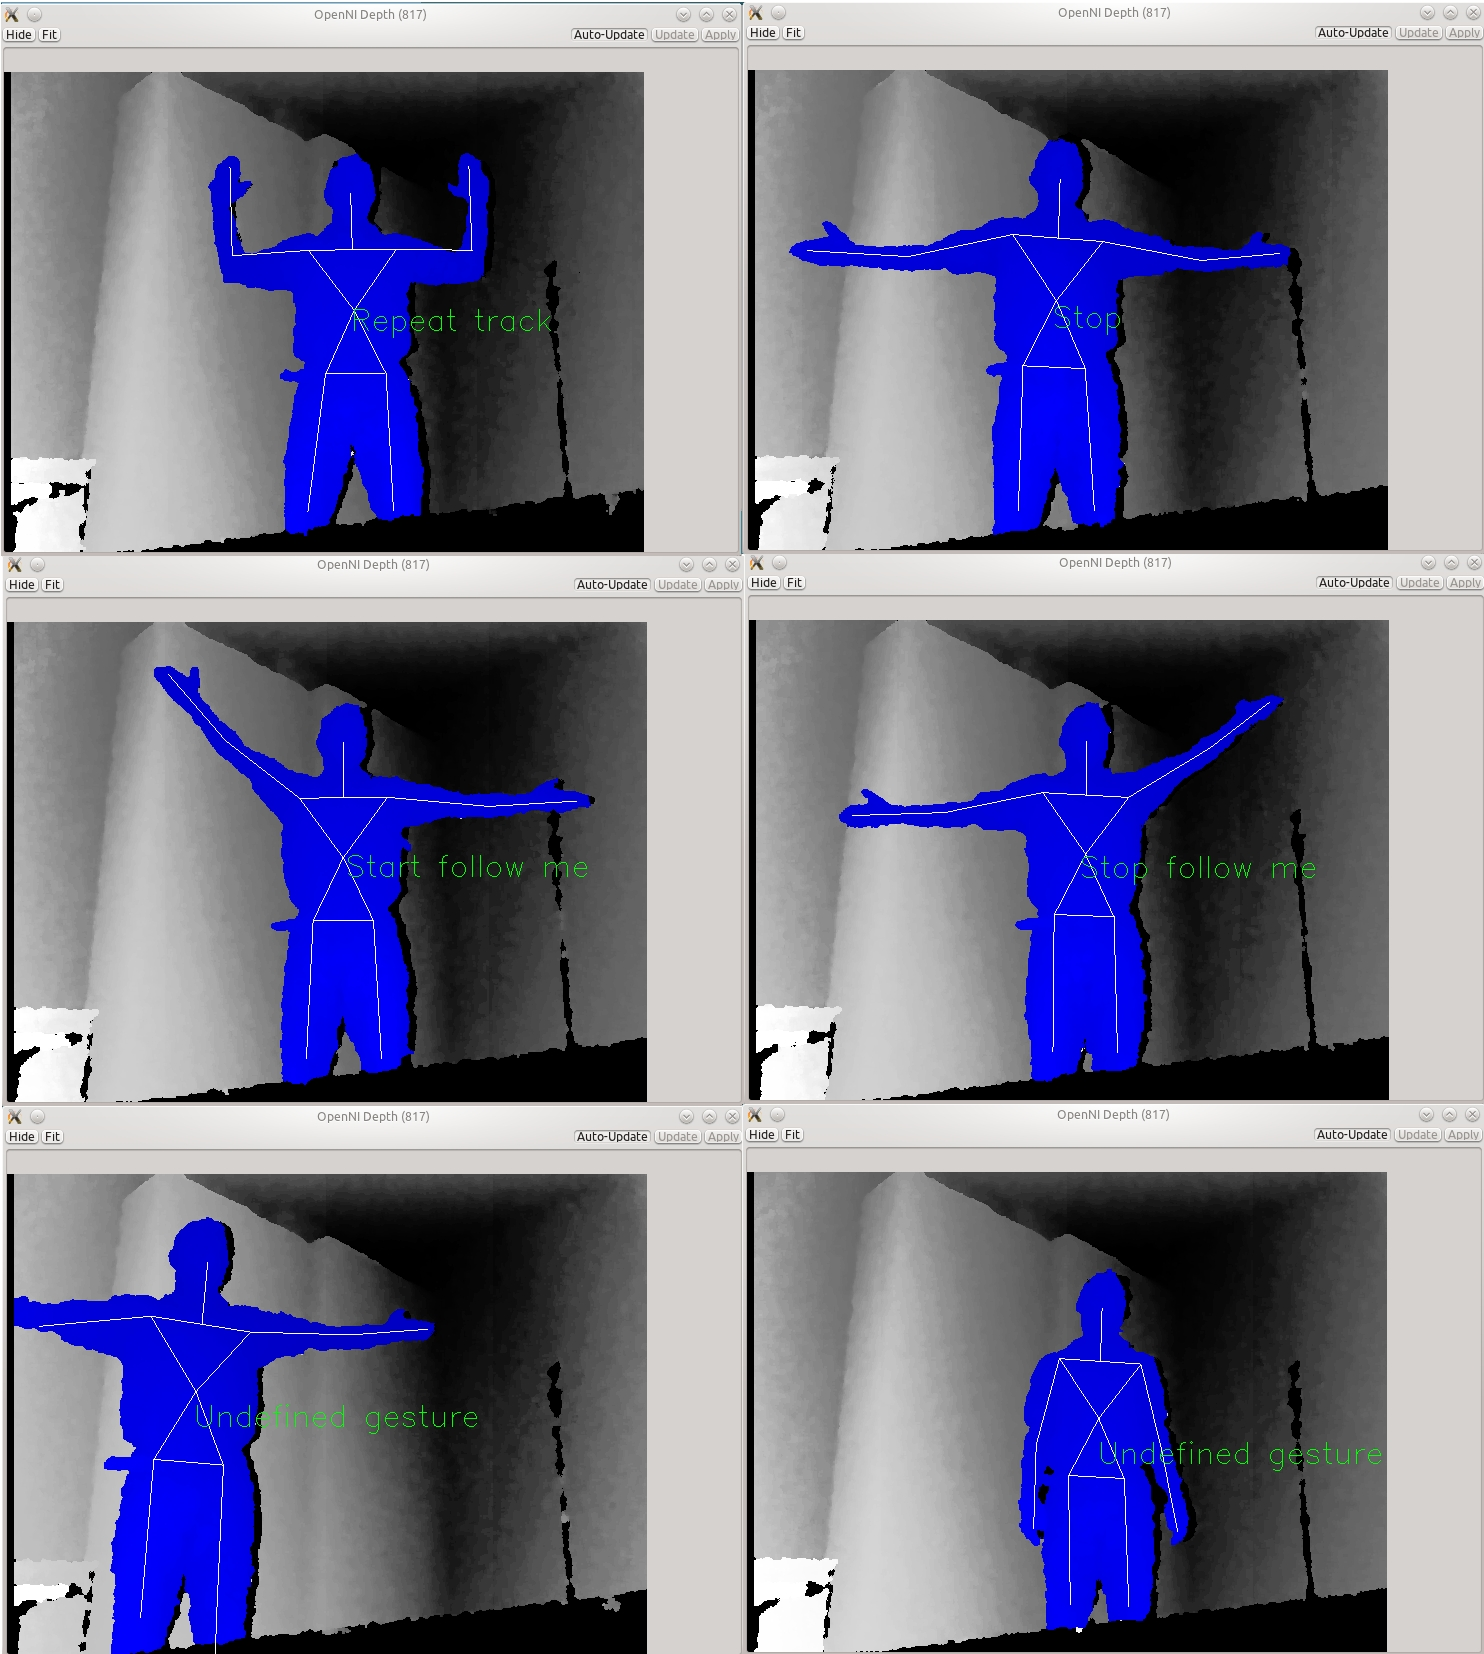
\includegraphics[scale=0.25]{graphics/Gesten.jpg}
\caption{\label{fig:Gesten} Die vier definierten Gesten (oben und in der Mitte),
 bzw. die beiden Möglichkeiten für unbestimmte Fälle (links unten: mangelndes Gelenk, rechts unten: normale Körperhaltung)}
\end{figure}

\begin{table}[h]
\centering
\begin{tabular}{ll}
angle\_alpha: & angle between elbow $\rightarrow$ shoulder $\rightarrow$ hip on
the left side\\
angle\_beta: & angle between elbow $\rightarrow$ shoulder $\rightarrow$ hip on
the right side\\
angle\_gamma: & angle between shoulder $\rightarrow$ elbow $\rightarrow$ hand on
the left side\\
angle\_delta: & angle between shoulder $\rightarrow$ elbow $\rightarrow$ hand on
the right side\\
angle\_epsilon: & angle between neck $\rightarrow$ shoulder $\rightarrow$ elbow
on the left side\\
angle\_fi: & angle between neck $\rightarrow$ shoulder $\rightarrow$ elbow on
the right side\\
left\_hand\_z: & height of left hand (palm)\\
right\_hand\_z: & height of right hand (palm)\\
\end{tabular}
\caption{Erklärung zu charakteristischen Markmalen (Winkeldefintionen)}
\label{tab:Winkeldefintionen}
\end{table}

Falls eines der relevanten Gelenke verdeckt ist oder keine verfolgbare Person im
Sichtbereich der Kamera ist, wird automatisch \lstinline{UNDEFIED_GESTURE}
zurückgegeben. Dies ist eine vorbeugende Maßnahme gegen falsche Berechnungen.

Eine weitere Möglichkeit der Umsetzung ist das Erkennen des zeitlichen Verlaufs von Gesten (bspw. Winken, Kreisen).
 In OpenNI und NITE Modulen wurden solche Funktionen implementiert, jedoch konnten wir diese aufgrund von Konfigurationsproblemen nicht nutzen.
Bei der Anwendung werden stets einzelne Personen verfolgt. Sollten sich mehrere Personen im Sichtfeld der Kamera aufhalten, wird nur die zuerst getrackte Person beachtet.

\subsection{Fazit}
Im Mobile Roboter -- Praktikum hatten wir die Gelegenheit aktuelle
 Forschungsgebiete der Servicerobotik zu beleuchten und verschiedene
 Technologien praktisch auszuprobieren. Es fiel besonders auf, dass viele Konzepte zwar theoretisch funktionieren,
 jedoch in der der Praxis nicht umsetzbar waren. Dies bedingte einige Iterationen im ursprünglichen Zielsystem des Projekts
 wodurch der Funktionsumfang der letztendlichen Roboterplattform weitaus geringer ausfiel als geplant.
 Besonders in der Bildverarbeitung gab es erhebliche Probleme, da Softwarebibliotheken eingesetzt werden sollten,
 die sich selbst noch stark in der Entwicklung befanden. Somit konnte zum Beispiel die in NITE implementierte Gestenerkennung
 nicht verwendet werden und die Sensordaten der Kinect waren weitaus stärker verrauscht als erwartet.
 
Die Aufteilung der Gruppe in drei spezialisierte Teilgruppen war bei dem Umfang des Projekts sehr sinnvoll,
 das Projektmanagement jedoch schlecht. In den Teams wurde es versäumt früh feste Strukturen und Arbeitsweisen zu implementieren wodurch
 wenig zielorientiertes Arbeiten und großer Motivationsschwund entstanden. Letztendlich konnte das Ziel des Projekts jedoch erreicht werden.


\chapter{Integration}
\label{integration_cha}
\authorsection{\editorjulian}
\todo[inline]{Julian: Schreiben}

\section{Aufgabenstellung}
\label{aufgabenstellung_integration_sec}

\begin{itemize}
\item Überblick was alles unter Integration fällt
\item Zusammenführen der einzelnen Teilprojekte
\item Zustandsmaschinen zur Steuerung/Beobachtung der einzelnen Teile
\item Planer um auf Umwelteinflüsse zu reagieren
\item Userinterface zur Steuerung des Roboters
\end{itemize}

Die Aufgaben im Bereich der Integration lassen sich in die folgenden Unterpunkte einordnen:

\begin{description}
\item[Code Zusammenführen]
Um das Auseinanderdriften der einzelnen Teilprojekte zu vermeiden ist ein regelmäßiges Zusammenführen mittels Git notwendig. Zusätzlich ist die Integration von Code der außerhalb des SegwayOmni-Projektes entsteht, wie etwa der Kinect Anteil, notwendig. Weiterhin muss die Kompatibilität der Schnittstellen zwischen den Teilprojekten gepflegt werden.

\item[Benutzerschnittstelle]
Zur Kontrolle des Roboters durch Benutzer muss eine Benutzerschnittstelle implementiert werden die es erlaubt die einzelnen Funktionen der Software zu aktivieren.

\item[Reaktion auf Zustandsänderungen]
Der vorherrschende Umweltzustand muss erkannt und eine entsprechende Reaktion ausgeführt werden.
\end{description}




\section{Grundlagen der Planung}
\label{grundlagen_integration_sec}

\begin{itemize}
\item Generell Planen: sense -> plan -> act (loop)
\item Unterschiedliche Problemstellungen
\item Mögliche Ansätze
\item State of the Art
\end{itemize}



\section{Umsetzung}
\label{umsetzung_integration_sec}

\subsection{Architektur}
\label{integration_architektur_sec}

\begin{itemize}
\item Highlevel Architektur, insbesondere Zusammenspiel Planer, Bahnplanung, Kinect
\item Aufteilung in sense und control
\item Bild!
\end{itemize}

\subsection{Planer}
\label{planer_integration_sec}

\begin{itemize}
\item Einordnung des konkreten Problems mit Attributen (siehe RobI F20):
\begin{itemize}
\item Determinismus
\item Endlicher Zustandsraum
\item Diskreter Zustandsraum
\item Statischer Zustandsraum
\end{itemize}
\item Umsetzung mit Zustandsmaschine
\item Sense Plan Act loop konkret
\end{itemize}

\subsection{Benutzerschnittstelle}
\label{benutzerschnittstelle_integration_cha}

\begin{itemize}
\item Ausführbare Handlungen
\item Steuerung über Gesten
\item Ausführen der entsprechenden Handlung
\item Steuerung der einzelnen Statemachines
\end{itemize}

\section{Probleme}
\label{probleme_integration_sec}

\begin{itemize}
\item Definition der Schnittstellen
\item Definition der Funktionen des Roboters
\end{itemize}


\chapter{Test auf realem Roboter}
\authorsection{\editortobias}

% \begin{itemize}
% 	\item Test auf realem Roboter erst spät möglich
% 	\item Schwer einzelne Komponenten zu testen da es viele Abhängigkeiten gibt
% 	\item Insbesondere der Steuerungs/Bahnplanungs/Hindernis Teil ist sowohl von den Laserscannern als auch vom Kinect-Teil abhängig.
% \end{itemize}


Nachdem die Ergebnisse der verschiedenen Gruppen in den Haupt-Entwicklungsstrang integriert sind, kann nach mehrmonatigem Testen in der Simulation mit Tests auf der realen Roboterplattform begonnen werden.

Ein Test mit \gls{hollie} zu einem früheren Zeitpunkt ist aufgrund der Abhängigkeiten zwischen den Komponenten nicht möglich.
Insbesondere das \lstinline{SegwayOmniBehaviours}-Modul, welches die Steuerung, Bahnplanung, sowie Kollisionsvermeidung übernimmt, ist beispielsweise sowohl von der Lokalisierung als auch von der Kinect abhängig.

Im Folgenden werden die Testumgebung sowie die während der Testphase aufgetretenen Schwierigkeiten beschrieben.


\section{Testumgebung}

% \begin{itemize}
% 	\item Aufgebaute Umgebung
% 	\begin{itemize}
% 		\item FZI, oberes Stockwerk
% 		\item erste Tests in Bereich ohne Hindernisse
% 		\item Abgegrenzter Bereich zur Simulation einer Büroumgebung (Siehe Motivation!)
% 		\item Karte erstellen zur Lokalisierung
% 	\end{itemize}
% 	\item Geplantes Bewegungs-Szenario
% \end{itemize}

Als Testumgebung dient das Obergeschoss im Gebäude des \gls{fzi}.
Erste Tests werden in einem weitläufigen Bereich ohne Hindernisse durchgeführt (s. Abb. \ref{fig:fzi_og}).
\begin{figure}
	\centering
	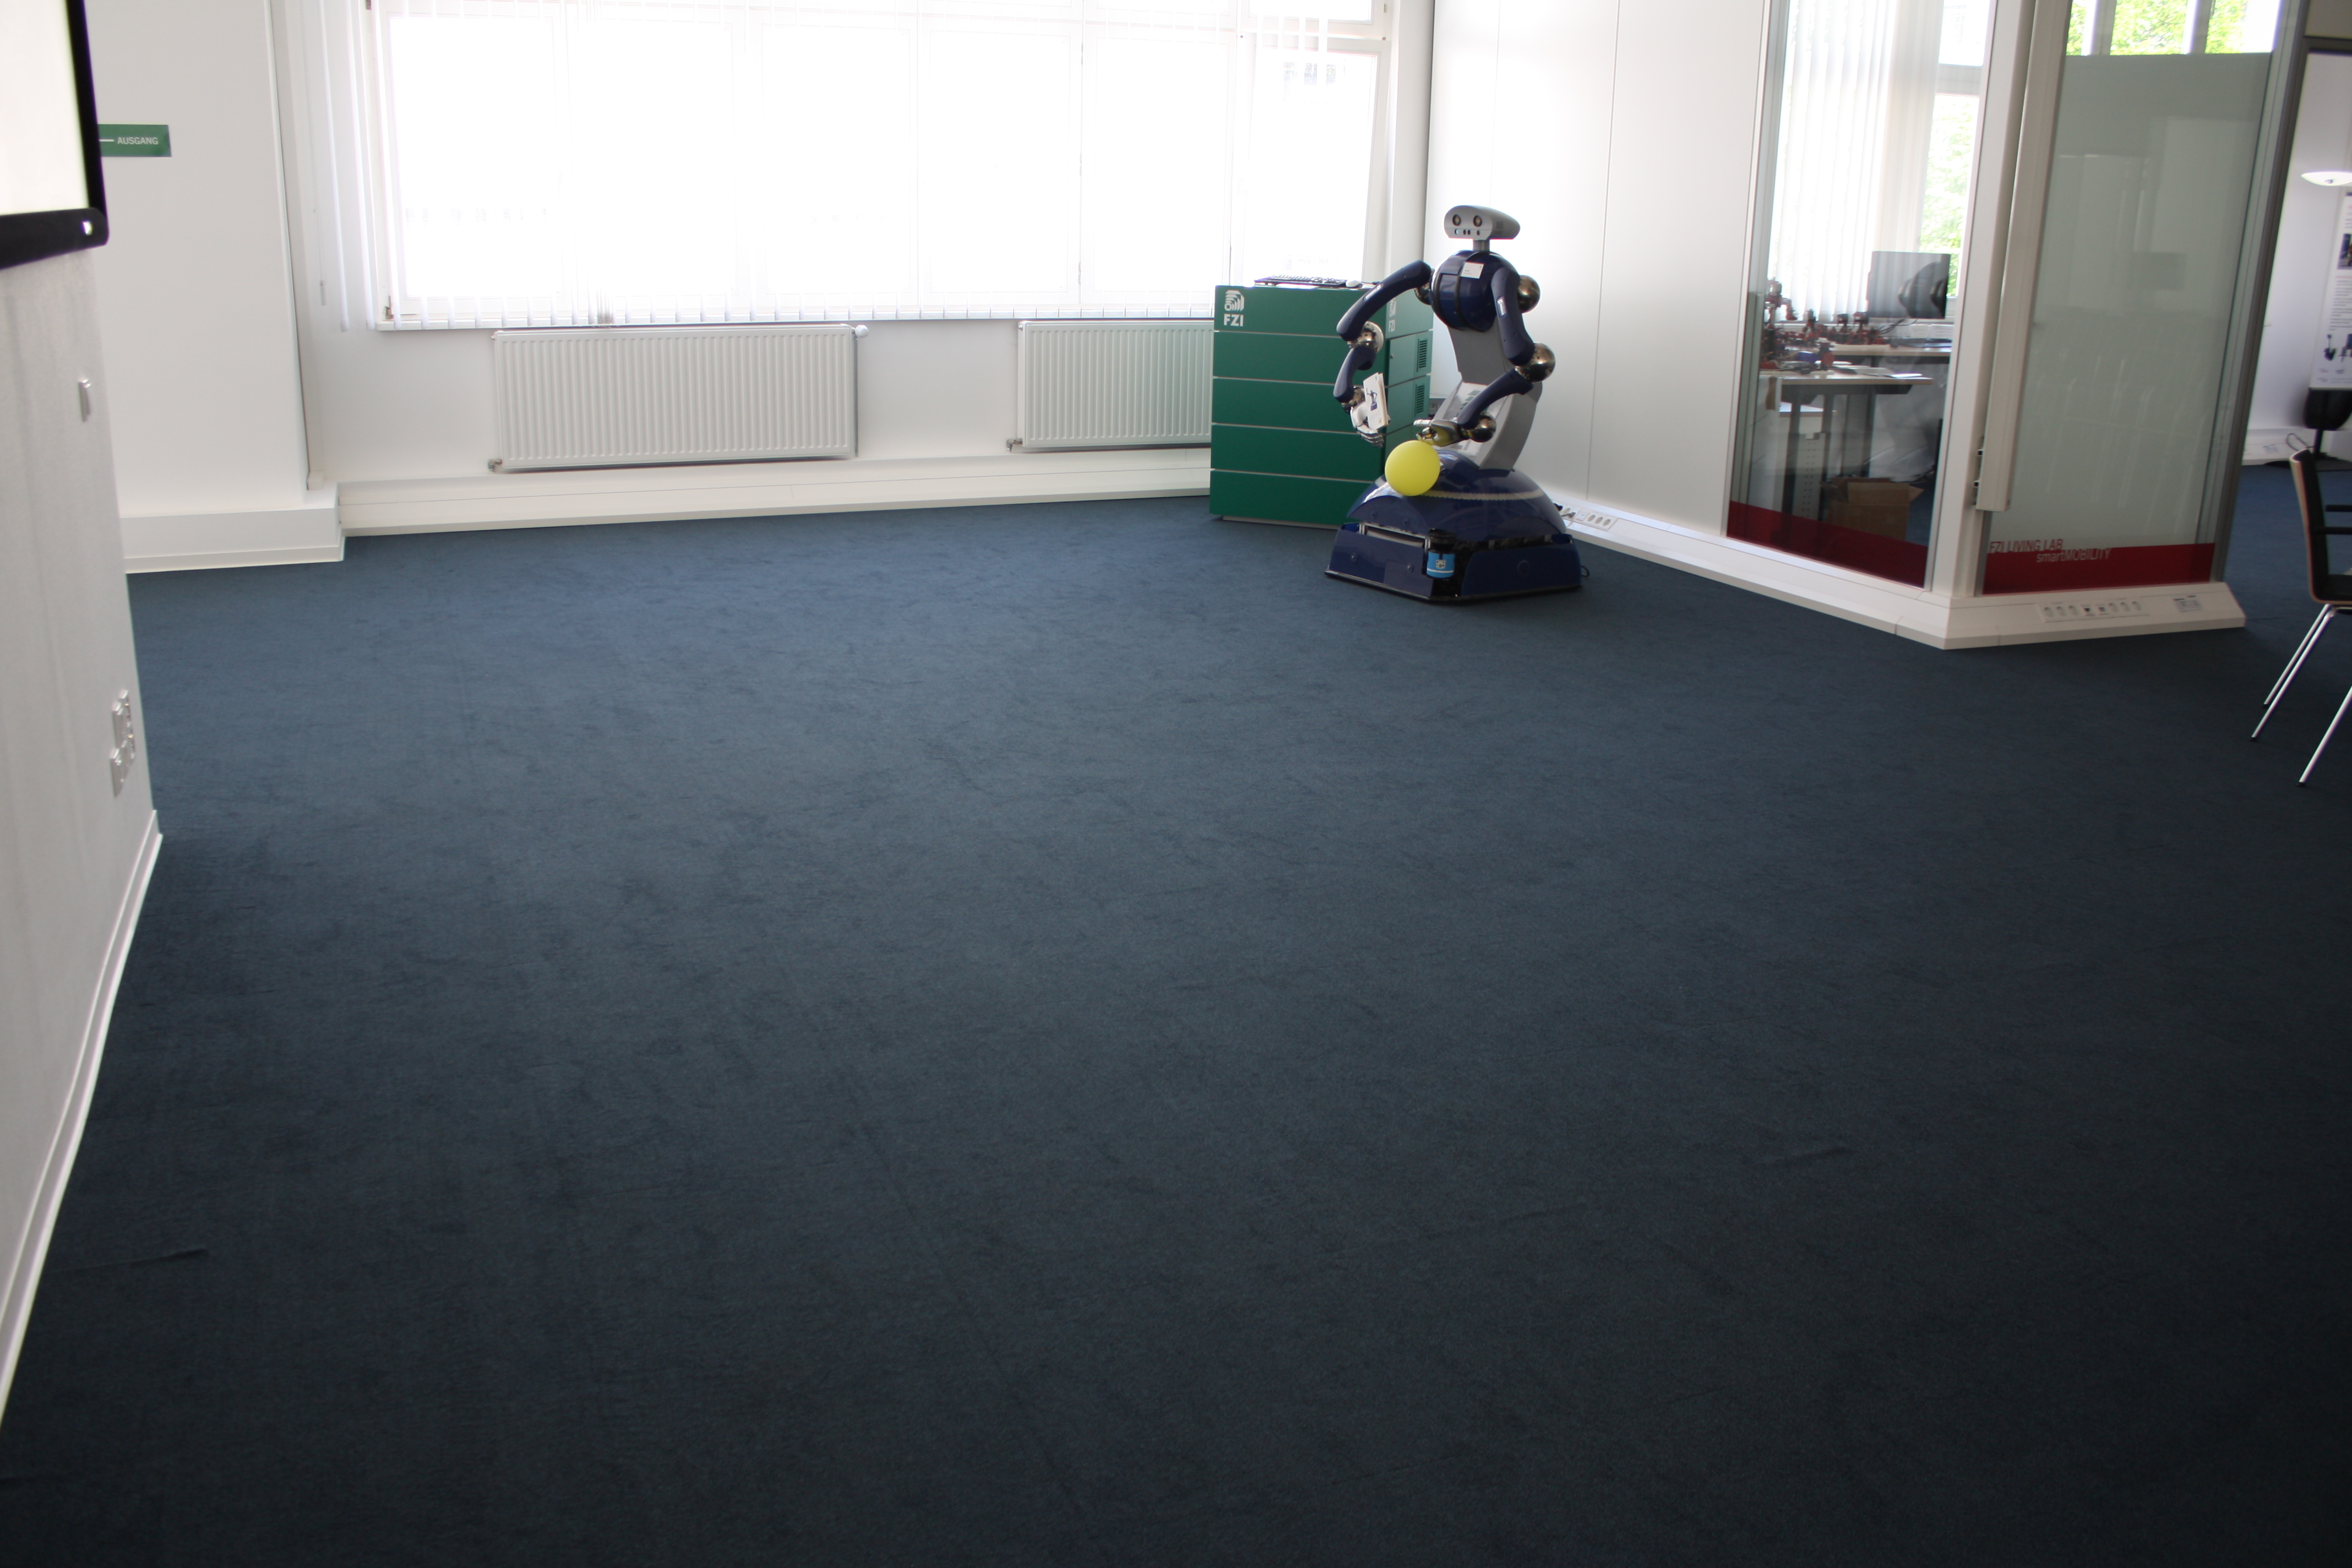
\includegraphics[width=0.7\textwidth]{graphics/fzi_og}
	\caption{Testbereich im Obergeschoss des \protect\gls{fzi}}
	\label{fig:fzi_og}
\end{figure}

Für weitergehende Tests (Lokalisierug, Hindernis-Umfahrung etc.) wird ein abgegrenzter Bereich zur Simulation einer Büroumgebung eingerichtet.
Dazu werden drei fest stehende Objekte auf einer rechtwinkligen Fläche platziert, die im entsprechenden Kartenmaterial ebenfalls verzeichnet sind (s. Abb \ref{fig:map_fzi}).
Diese Objekte ermöglichen eine Lokalisierung des Roboters in der Umgebung.
Als Hindernis dient eine einfach Plastik-Mülltonne (welche selbstverständlich nicht in der Karte verzeichnet ist).

\begin{figure}[h]
  \centering
  \subfloat[Geplante Umgebung]{\label{fig:map_fzi_plan}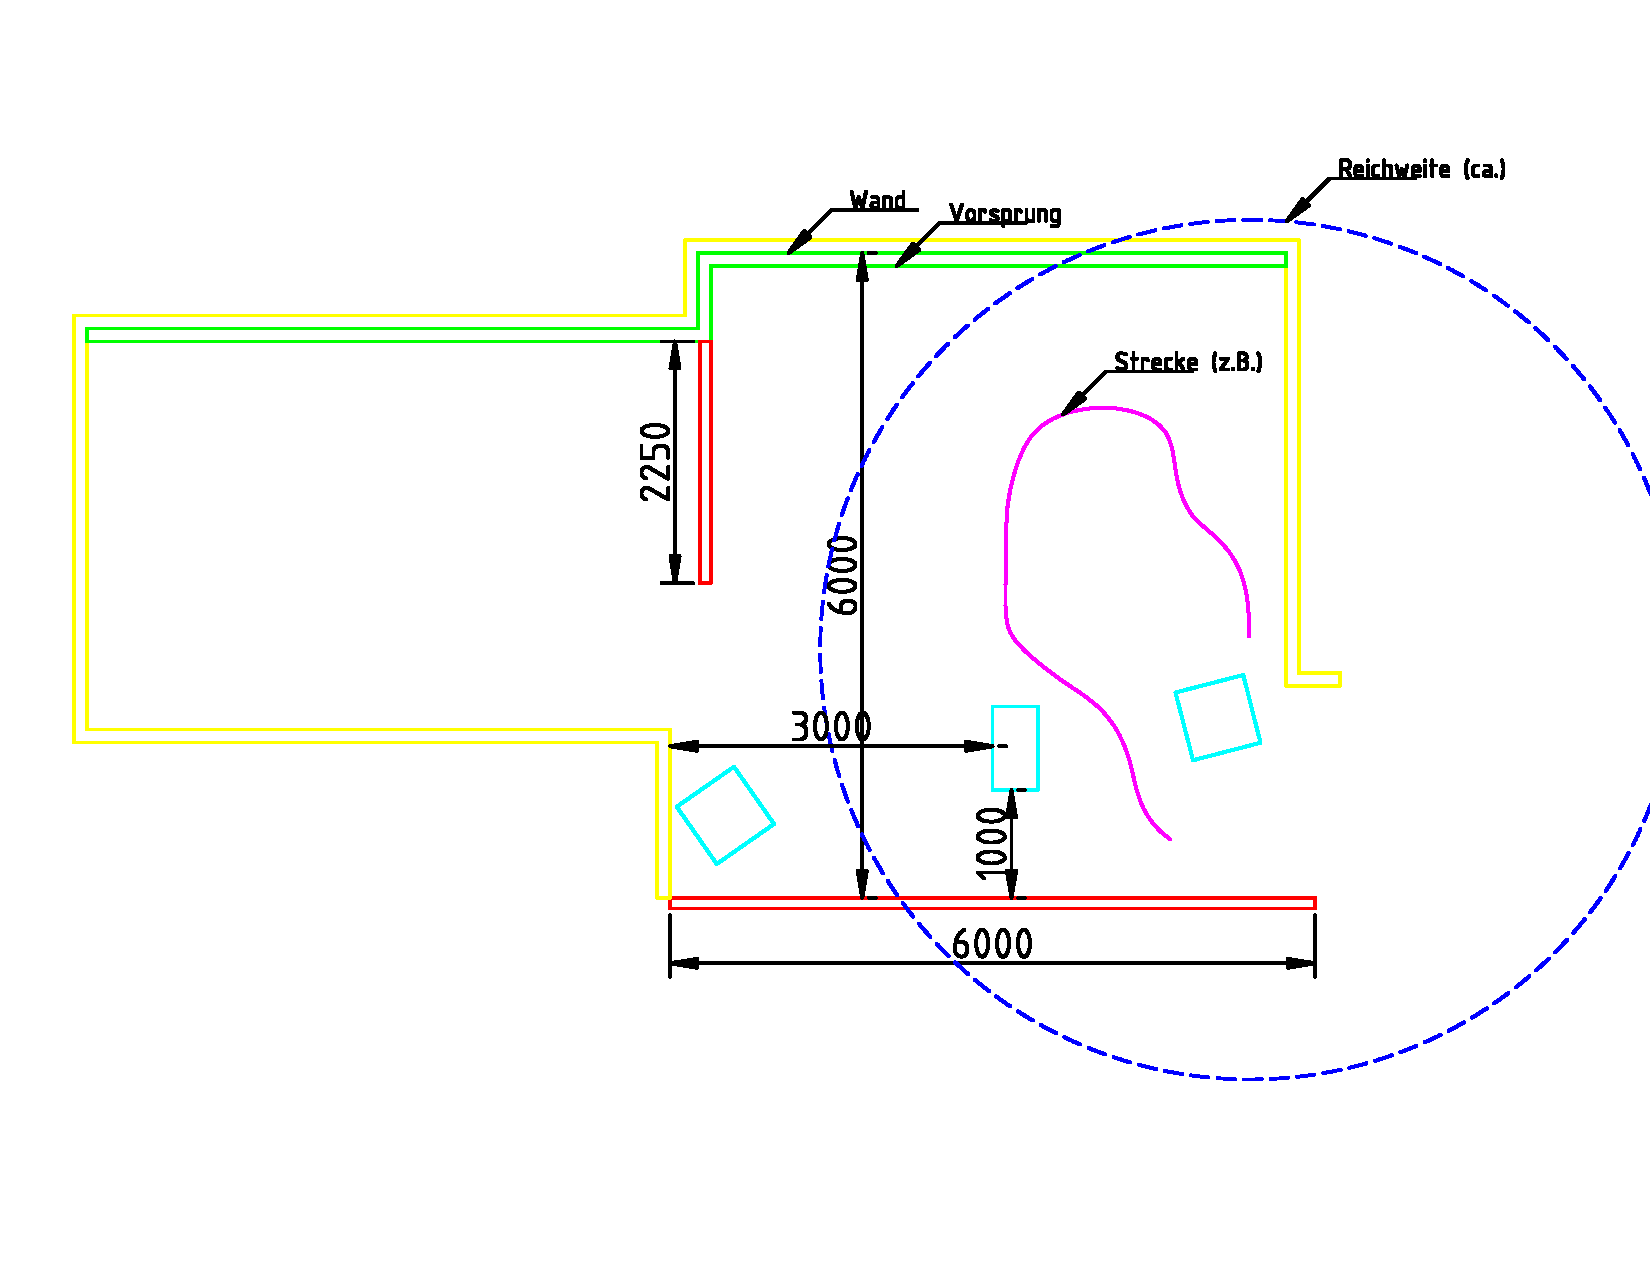
\includegraphics[width=0.45\textwidth]{graphics/map_fzi_plan}}
  \quad %add desired spacing between images, e. g. ~, \quad, \qquad etc. (or a blank line to force the subfig onto a new line)
  \subfloat[Umgebung mit \protect\gls{hollie} und realen Scannerdaten]{\label{fig:map_fzi_hollie}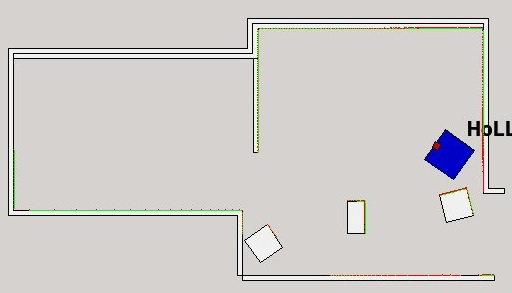
\includegraphics[width=0.4\textwidth]{graphics/map_fzi}}
  \caption{Simulierte Büroumgebung für weitere Tests}
  \label{fig:map_fzi}
\end{figure}

In dieser Umgebung soll der Roboter folgendes Szenario erfüllen können:
\begin{enumerate}
  \item Person folgen ohne Hindernis
  \item Rückfahrt zum Start ohne Hindernis
  \item Pfad abfahren mit Hindernis
\end{enumerate}



\section{Aufgetretene Schwierigkeiten}

\subsection{Laserscanner}
\label{test_schwierigkeiten_laserscanner_sec}

Der Test der auf \gls{hollie} montierten Laserscanner gestaltet sich zu Beginn schwierig.
Die zwei aufgetretenen Probleme werden im Folgenden erläutert.

\subsubsection{\glqq Unsichtbare Wand\grqq}

Das erste \emph{Problem} wird von den Praktikumsteilnehmern gerne als \glqq unsichtbare Wand\grqq\ bezeichnet.
Hintergrund dieser Namensschöpfung ist, dass sich die Scanner-Daten zwar auslesen und auch in der Benutzeroberfläche (\lstinline{mcagui}) anzeigen lassen, jedoch befindet sich in ca. $4m$ Entfernung ein großes, nur sehr leicht gekrümmtes Objekt, was von einem der beiden Scanner erkannt wird.
Auf dem Scanner-Bild erscheint diese Linie wie eine Wand (s. Abb. \ref{fig:scanner_problem}).
Leider ist in der Realität an dieser Stelle keine Wand, sondern lediglich freier Raum.

\begin{figure}[h]
	\centering
	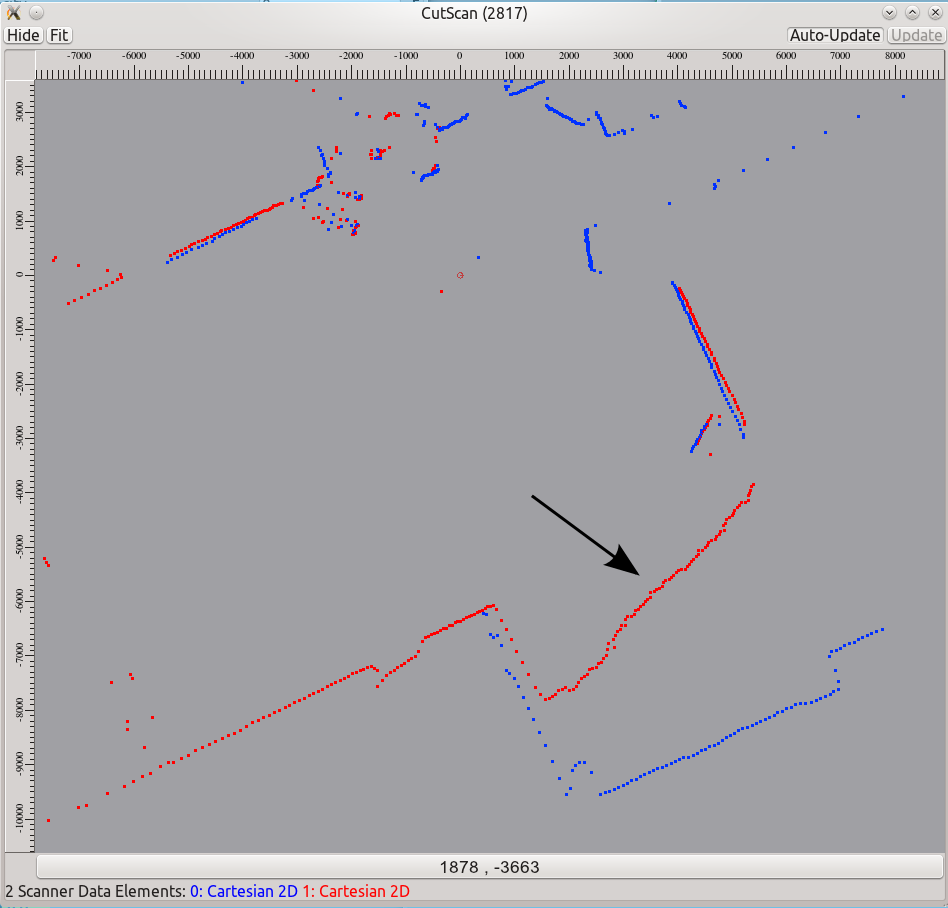
\includegraphics[width=0.7\textwidth]{graphics/cutscan_fehler}
	\caption[\glqq Unsichtbare Wand\grqq]{Problem der \glqq unsichtbaren Wand\grqq\ im Scanner-Bild: Die \glqq Wand\grqq\ ist mit einem Pfeil gekennzeichnet}
	\label{fig:scanner_problem}
\end{figure}
%\todoprivate{Tote Pixel auch noch einzeichnen}

Die \emph{Ursache} dieser Erscheinung ist die Montage des Laserscanners am Roboter.
Da dieser nicht exakt waagerecht an \gls{hollie} angebracht ist, verläuft die Scan-Ebene nicht exakt parallel zum Untergrund.
Daher erreicht ca. die Hälfte der Scanner-Strahlen in einiger Entfernung den Boden, anstatt parallel zum Boden zu verlaufen.
In der grafischen Darstellung der Messpunkte ähnelt dies dann einer Wand, da die Scanner-Strahlen den Boden alle in nahezu der gleichen Entfernung treffen.

Nach Klärung der Ursache der \glqq unsichtbaren Wand\grqq\ erscheint das Problem für die weiteren Tests nicht relevant, da eine Sichweite der Laserscanner von $4m$ ausreichend ist.
Eine \emph{Lösung} ist daher nicht nötig.


\subsubsection{\glqq Tote Pixel\grqq}

Die zweite \emph{Problematik} im Zusammenhang mit den Laserscannern sind einige scheinbar \glqq tote Pixel\grqq.
Dies sind Scan-Punkte, die anhand der grafischen Darstellung offensichtlich einen Gegenstand sehr nahe an oder sogar innerhalb der Laserscanner zurückgeben.
Dieses Problem tritt bei beiden Scannern auf, und betrifft einen geringen Bruchteil der Scanner-Strahlen.
Schwierig für \gls{hollie} ist dies deshalb, da der Roboter quasi immer in einem Hindernis steht.
Somit ist es dem A*-Algorithmus (s. Abs. \ref{kollisionsvermeidung_subsec}, S. \pageref{kollisionsvermeidung_subsec} f.) nicht möglich, eine Trajektorie um das Hindernis zu planen.
Als Folge dessen, bleibt \gls{hollie} auf der Stelle stehen, und bewegt sich nicht.

Die \emph{Ursache} dieses Problems liegt in einer unglücklich gewählten Behandlung für Scan-Punkte, die eine Fehlmessung zurückgeben.
Diese Punkte werden bis dato mit dem Wert 0 belegt.
Da dies einen Gegenstand in der Entfernung 0 bedeutet, liegen diese Scan-Punkte wie vermutet tatsächlich innerhalb der Laserscanner.

Ein erster \emph{Lösung}sversuch, gewisse Scan-Bereiche für die weiteren Berechnungen einfach zu ignorieren, scheitert an der Tatsache, dass nicht immer exakt die gleichen \glqq toten Pixel\grqq\ auftreten.
Da allerdings die angesprochene Belegung mit dem Wert 0 nicht bereits in der Laserscanner-Software, sondern innerhalb der Scanner-Library auf \gls{hollie} geschieht, ist dies die Stelle, an welcher das Problem behoben werden kann:
Anstatt dem Wert 0 werden nun Fehlmessungen mit einem hinreichend großen Wert belegt, sodass die Scan-Strahlen mit Fehlmessungen nun in weiter Entfernung vom Roboter liegen.
Die \glqq toten Pixel\grqq\ bereiten damit keine Schwierigkeiten mehr.


%\begin{itemize}
%	\item \glqq Unsichtbare Wand\grqq\ in ca. 4m Entfernung
%	\begin{itemize}
%		\item Scanner nicht exakt waagerecht angebracht
%		\item nicht relevant, da Entfernung von 4m ausreichend
%	\end{itemize}
%	\item \glqq Tote Pixel\grqq\
%	\begin{itemize}
%		\item Fehlmessungen werden mit Wert 0 und nicht MAX belegt
%		\item Roboter steht immer im Hindernis -> keine Fortbewegung
%		\item Optionale Zuschaltung der Module per XML
%	\end{itemize}
%\end{itemize}



\subsection{Stromversorgung}

Ein weiteres Problem, welches beim ersten Test mit der realen Roboterplattform auftritt, ist die Stromversorgung.
Die Akkus, die auf \gls{hollie} verbaut sind, sind derzeit nicht in der Lage sowohl den Roboter selbst als auch die darauf montierte Kinect-Kamera (s. Abs. \ref{kinect_grundlagen_sec}, S. \pageref{kinect_grundlagen_sec} ff.) mit genügend Strom zu versorgen.
Dies äußert sich darin, dass die Kinect sich im Akku-Betrieb nicht in Betrieb nehmen lässt.

Daher ist es notwendig, ein externes Netzgerät zu verwenden, und den Roboter so mit zusätzlichem Strom zu versorgen.
Dies hat allerdings zur Folge, dass die Reichweite von \gls{hollie} durch die Länge des Kabels zwischen Roboter und externem Netzgerät beschränkt ist.
Der Aktionsradius beträgt somit nur noch ca. \unit[5]{m}.

Für die Zwecke des Praktikums ist diese Reichweite mit wenigen Einschränkungen ausreichend.

%\begin{itemize}
%	\item Robotereigene Stromversorgung reicht nicht aus für Roboter + Kinect
%	\item Netzgerät nötig
%	\item Einschränkung der Reichweite
%\end{itemize}



\subsection{Kinect}
\label{test_kinect}

Nach ersten Erfolgen mit dem realen Roboter stellt sich heraus, dass die Kinect-Kamera (s. Abs. \ref{kinect_grundlagen_sec}, S. \pageref{kinect_grundlagen_sec} ff.) \emph{Schwierigkeiten} damit hat, selbst bewegt zu werden und gleichzeitig auch noch einen sich wiederum auch bewegenden Menschen zu tracken.
Wenn \gls{hollie} sich zügig durch den Raum bewegt, kommt es bei der Kamera häufig zu einem Verlust des getrackten Menschen.
Oft werden auch andere Objekte (beispielsweise Säulen im Raum, Fenster, oder ähnliches) als \glqq Tracking-Kandidaten\grqq\ erkannt und hervorgehoben.
Dieses Phänomen zeigt sich auch bei rein rotatorischen Bewegungen.

Andere wissenschaftliche Mitarbeiter am \gls{fzi} haben bereits ähnliche Beobachtungen mit der Kinect gemacht.
Die \emph{Ursache} dafür liegt wohl darin, dass die Kinect ursprünglich als Einheit für den stationären Gebrauch entwickelt wurde.
\Dh die Kamera steht üblicherweise fest auf einem Tisch \oae, und lediglich der Mensch vor der Kamera bewegt sich.
Im vorliegenden Fall einer sich bewegenden Kinect bewegt sich ja aus Sicht der Kamera nahezu alles im Sichtfeld (dazu gehören neben dem Menschen auch sämtliche Hintergrundobjekte etc.).
Dies scheint eine fehlerfreie Fokussierung des Menschen sehr zu limitieren.

Da eine \emph{Lösung} dieses Problems außerhalb der Möglichkeiten der Praktikumsteilnehmer liegt, wird ein \glqq work-around\grqq\ eingesetzt:
Die Geschwindigkeiten, mit denen sich \gls{hollie} fortbewegt, werden auf niedrigere Werte beschränkt.
Dazu gehören sowohl die translatorischen als auch die rotatorischen Geschwindigkeiten.
Dadurch kann die beschriebene Problematik zwar nicht endgültig beseitigt werden, die Häufigkeit des Auftretens wird jedoch reduziert.

%\begin{itemize}
%	\item verliert getrackten Menschen bei zu schneller Bewegung (insbesondere Rotation)
%	\item Verringerung der Geschwindigkeit (Rotation sowie Translation)
%\end{itemize}



\subsection{Weitere Probleme}

Schließlich treten während den Tests auf der realen Roboterplattform auch noch einige weitere, kleinere Probleme auf, von denen hier nur einige kurz erwähnt werden sollen.

Eine sehr wichtige Erkenntnis während der Testphase war es, dass einzelne Module unbedingt anhand einer externen Konfigurationsdatei (beispielsweise eine \lstinline{XML}-Datei) aktivierbar bzw. deaktivierbar sein sollten.
Falls dies nur innerhalb des programmierten Codes, also nur zur Compile-Zeit möglich ist, so kostet das ständige Ändern des Codes, Neu-Bauen der Software, Überspielen auf den Roboter etc. einen immensen Zeitaufwand!
Durch einfache \lstinline{bool}-Flags in der Konfigurationsdatei können die einmal erzeugten Binärdaten weiter verwendet werden, und dennoch bestimmte Module einfach de-/aktiviert werden.
Der zusätzliche Aufwand während der Programmierung ist sehr gering, die Zeitersparnis während der Testphase jedoch immens.

Aufgrund des weichen Bodens im Obergeschoss des \gls{fzi} kann der Roboter nur sehr ungenaue Odometrie-Daten liefern.
Die Mecanum-Räder haben auf diesem Untergrund großen Schlupf.
So kommt es vor, dass \gls{hollie} auf einer Fahrstrecke von ca. \unit[8]{m} bereits durchaus einen Fehler in der odometrischen Lokalisierung von mehr als \unit[2]{m} hat.
Der Grund hierfür liegt in der sehr langsamen Fortbewegungsgeschwindigkeit, mit welcher der Roboter betrieben wird.
Bewegt man \gls{hollie} schneller, so verbessern sich die Werte der odometrischen Lokalisierung deutlich.
Da die Geschwindigkeit aufgrund anderer Faktoren (vgl. Abs. \ref{test_kinect}) begrenzt ist, ist eine Lokalisierung allein auf Basis der Odometrie-Daten somit unmöglich.

Weiterhin treten auch noch viele kleinere bis mittelschwere Fehler in der während des Praktikums programmierten Software auf, auf die nicht näher eingegangen wird.

% \begin{itemize}
% 	\item Odometrie auf Teppichboden
% 	\item Abschaltung von Modulen
% 	\item SW-Bugs
% 	\item \ldots
% \end{itemize}


\chapter{Fazit}

\section{Erreichte Ziele}
\authorsection{\editordummy}
\todo[inline]{Steuerungs-Gruppe: Schreiben}

\section{Ausblick}
\authorsection{\editordummy}
\todo[inline]{Kinect-Gruppe: Schreiben}

\section{Reflexion}
\authorsection{\editordummy}
\todo[inline]{Anne+Andreas: Schreiben}

% -----------------------------------------------------------------------------
%													Organisatorische Herausforderungen
\subsection{Organisatorische Herausforderungen}

Umsetzung der Form Großes Projekt, Projektpraktikum daher komplette Planung im
Verantwortungsbereich der Gruppe beschreiben der sich daraus ergeben
herausforderungen

 Organisatorisch:
        Anfangs noch mehrere starke Änderungen an der SW-Umgebung
        Paralleles Arbeiten zunächst nicht möglich
        Roboter stand erst spät zur Verfügung
        Eingeschränkter Zugriff auf Roboter (Cebit, Review)
        Kein festgelegter Abgabetermin
        Kommunikation zwischen den Gruppen
        Mangelndes Projektmanagement
        Einhaltung der internen Deadlines
% -----------------------------------------------------------------------------
%													Fachliche Herausforderungen
\subsection{Fachliche Herausforderungen}

Geplante Punkte Unterschiedliche Vorraussetzungen, verstehen von großen
teilweise spärlich kommentiertem code

 Fachlich:
        Lange Einarbeitungszeit in MCA2
        Teilweise Probleme mit schlechter/fehlender Dokumentation des Sourcecodes
        Unterschiedliche Programmierkenntnisse innerhalb der Gruppen

% -----------------------------------------------------------------------------
%													Learned Lessons
\subsection{Learned Lessons}

Aus den Herausforderungenn erkannten Erkenntnisse sowie kurze Erläuterungen über
Simulation und Praxis unterschied


\pagestyle{scrplain}
\appendix

% \chapter{Analysenmethoden zur Bestimmung der Reaktionsvariablen }

\section{Gaschromatographie}

Die Bestimmung des Wasserstoffanteils mit dem GC HP-5880 A Series erfolgt durch eine Temperaturrampe. Zuerst wird die Temperatur fünf Minuten lang bei $50 ^{\circ}C$ gehalten. Danach wird bis $130 ^{\circ}C$ ($15 ^{\circ}C/min$) aufgeheizt. Der GC besaß eine gepackte Trennsäule (Porapak Q). Als Detektor stand ein Wärmeleitfähigkeitsdetektor (WLD) zu Verfügung. 
%kleiner Test, mal schauen ob ich immer noch commiten darf nach Github Accountname wechsel

Der GC HP 6890 ist mit zwei Säulen ausgestattet, eine für die Bestimmung von Wasserstoff (80/100 Hayesep Q, 2 m lang)  mit Stickstoff als Trägergas, und eine andere Säule (60/80 Molekularsieb, 4 m lang) für CO2, Stickstoff, Sauerstoff und Kohlenwasserstoffe ($< C4$), in der Helium als Trägergas benutzt wird. Für die Konzentrationsmessung wurde zwei Detektoren verwendet: ein Wärmeleitfähigkeitsdetektor (WLD) und ein Flammenionisationsdetektor (FID), die in Serie geschaltet waren. 

In dem WLD wird die Wärmeleitfähigkeit des Trägergases (Stickstoff) mit der der gaschromatographisch getrennten Substanzen verglichen. Der Vergleich erfolgt an einer Wheatstoneschen Brücken. Solange nur Trägergas durch die Wheatstoneschen Brücken fließt, wird die Wärme vollständig abgeführt. Wenn andere Substanzen mit geringe Leitfähigkeit in die Messzelle gelangen, entsteht ein Wärmestau am Hitzdraht (Platin), der den elektrischen Wiederstand erhöht. 

Für die anderen Komponenten in der Gasphase wird ein FID benutzt, der für Verbindungen mit C-H oder C-C Bindungen eine deutlich höhere Empfindlichkeit besitzt. Die Verbrennung der Komponenten läuft über die Bildung von Radikalen, durch die die Ionisation erhöht wird. 

Die Messung erfolgt während 31 Minuten. Die Temperatur wird von $60 ^{\circ}C$ auf $220 ^{\circ}C$ erhöht. Zuerst wird nach der Probeeinspritzung die Temperatur bei $60 ^{\circ}C$ zwei Minuten lang gehalten. Dann erfolgt eine Aufheizungsrate von $5 ^{\circ}C/min$  bis eine Temperatur von $160 ^{\circ}C$ erreicht wird. Anschließend steigt die Temperatur bis $220 ^{\circ}C$ mit einer Aufheizungsrate von $15 ^{\circ}C/min$. Bei $220 ^{\circ}C$ wird die Temperatur während  5 min konstant gehalten. 

Die Gasproben werden mit Gasspritzen aus zwei Probenehmern  gezogen.  Ein erster Probenehmer befand sich direkt an der Stelle der Phasentrennung, der zweite war hinter dem Abwasserbehälter angebracht. 
Zur Kalibrierung der Gas-Chromatographen wurden täglich Gasproben mit bekannter Zusammensetzung eingespritzt. Da die Gas-Chromatographen von mehreren Arbeitsgruppen bedient wurden, war eine Ausheizung des GC während mehreren Stunden nötig, die jedes zweites Wochenende durchgeführt wurde.  Die Versuchsplanung hängte davon ab, dass die Gasproben gemessen werden konnten.

\section{Analyse zur Bestimmung des Kohlenstoffgehalts im Abwasser}

TOC-Messgerät (DC-190 Rosemount-Dohrman) 

Das Messprinzip besteht aus einer hochtemperatur-katalysierten Verbrennung der Abwasserprobe. Die Verbrennung findet in einem Quarz-Rohr statt, das  gepackt mit dem Katalysator Pt/Al2O3 ist. Die Ofentemperatur  beträgt $800 ^{\circ}C$. Durch die katalysierte unterstützte Oxidierung mit reinem Sauerstoff ($250 ml/min$), werden die Abwasserproben vollständig zu CO2 und Wasser umgewandelt. Das entstehende CO2 wird von dem Wasser in einem Kondensator-Gas-Flüssig-Trennungssystem (Kupfer-Zinn-Adsorber) gereinigt. Die Halogene werden von dem Gasprodukt getrennt. Die reine CO2-Menge wird anhand eines Infrarotdetektors ermittelt. Anorganischer Kohlenstoff (IC) wird mit einem IC  Reaktor bestimmt, der Phosphorsäure 20 \% enthält. In diesem säuerlichen Medium werden die  anorganischen Carbonate der Abwasserprobe zu CO2 umgewandelt. Das entstehende Gas wird zum Trennungssystem geleitet und mit dem Infrarotdetektor gemessen. Die Genauigkeit dieses Messprinzips lag um etwa 2 \%. 

Küvetten-Test LCK 381 (Dr. Lange GmbH, Düsseldorf, D, Messbereich 60-735 mg/l)

Die Proben müssen verdünnt werden, wenn der Messbereich überschritten werden könnte.  Zur Bestimmung des Gesamtkohlenstoff-Gehaltes (TC) wurden $200 \mu l$ der verdünnten Abwasserprobe in die mit dem Aufschlussreagenz (Natriumperoxidsulfat) gefüllte TC-Küvette (KD 381 B) pipettiert. Nach dem Verschließen mit Originaldeckel und mehrmaligem Umschwenken wurde die TC-Küvette mit einer vorbereiteten Indikatorküvette (LCK 380/381) durch einen Membran-Doppel-deckel verbunden. Gleichzeitig wurde die TiC-Küvette (KE 381 B) mit $1 ml$ der Probe befüllt. Analog zur Aufarbeitung der TC-Bestimmung wurde die TiC-Küvette mit dem Originaldeckel verschlossen und mehrfach geschüttelt. Im Anschluß daran wurde die TiC-Küvette mit der entsprechenden Indikatorküvette verbunden. Beide Küvettenkombinationen wurden gleichzeitig in einem vorgeheizten Thermostaten LT 100 (Dr. Lange GmbH) 2 h bei $100^{\circ}C$ erwärmt. Während der Erwärmung reagieren die Abwasserproben mit dem Reagenz und es entsteht CO2, das den Indikator verfärbt. Nach dem Abkühlen auf Raumtemperatur wurden die Indikatorküvetten mit dem Spektralphotometer CADAS-200 (Dr. Lange GmbH) gemessen. Die Indikatorküvetten werden außen gut gesäubert und in den Photometer eingesetzt. Das Barcode-Ettiket wird von der CADAS-200 gelesen, dadurch werden die entsprechenden Wellenlängen für die Durchführung der Messung eingestellt.   



\listoffigures
\listoftables
\bibliography{content/bibliography}

\printindex


\end{document}
